\section{Non signal testing of the regular and variational Autoencoder}

\subsection*{Channel removing}
\subsubsection*{Autoencoder}
Both the large and small autoencoder produced results, and are shown below. The Higgs, singletop and ttbar channels have been selected here, as they are 
from a physics stand point the channels that looks most unlike the other channels.  


\begin{figure}[h!]
    \centering
    \begin{subfigure}{.45\textwidth}
        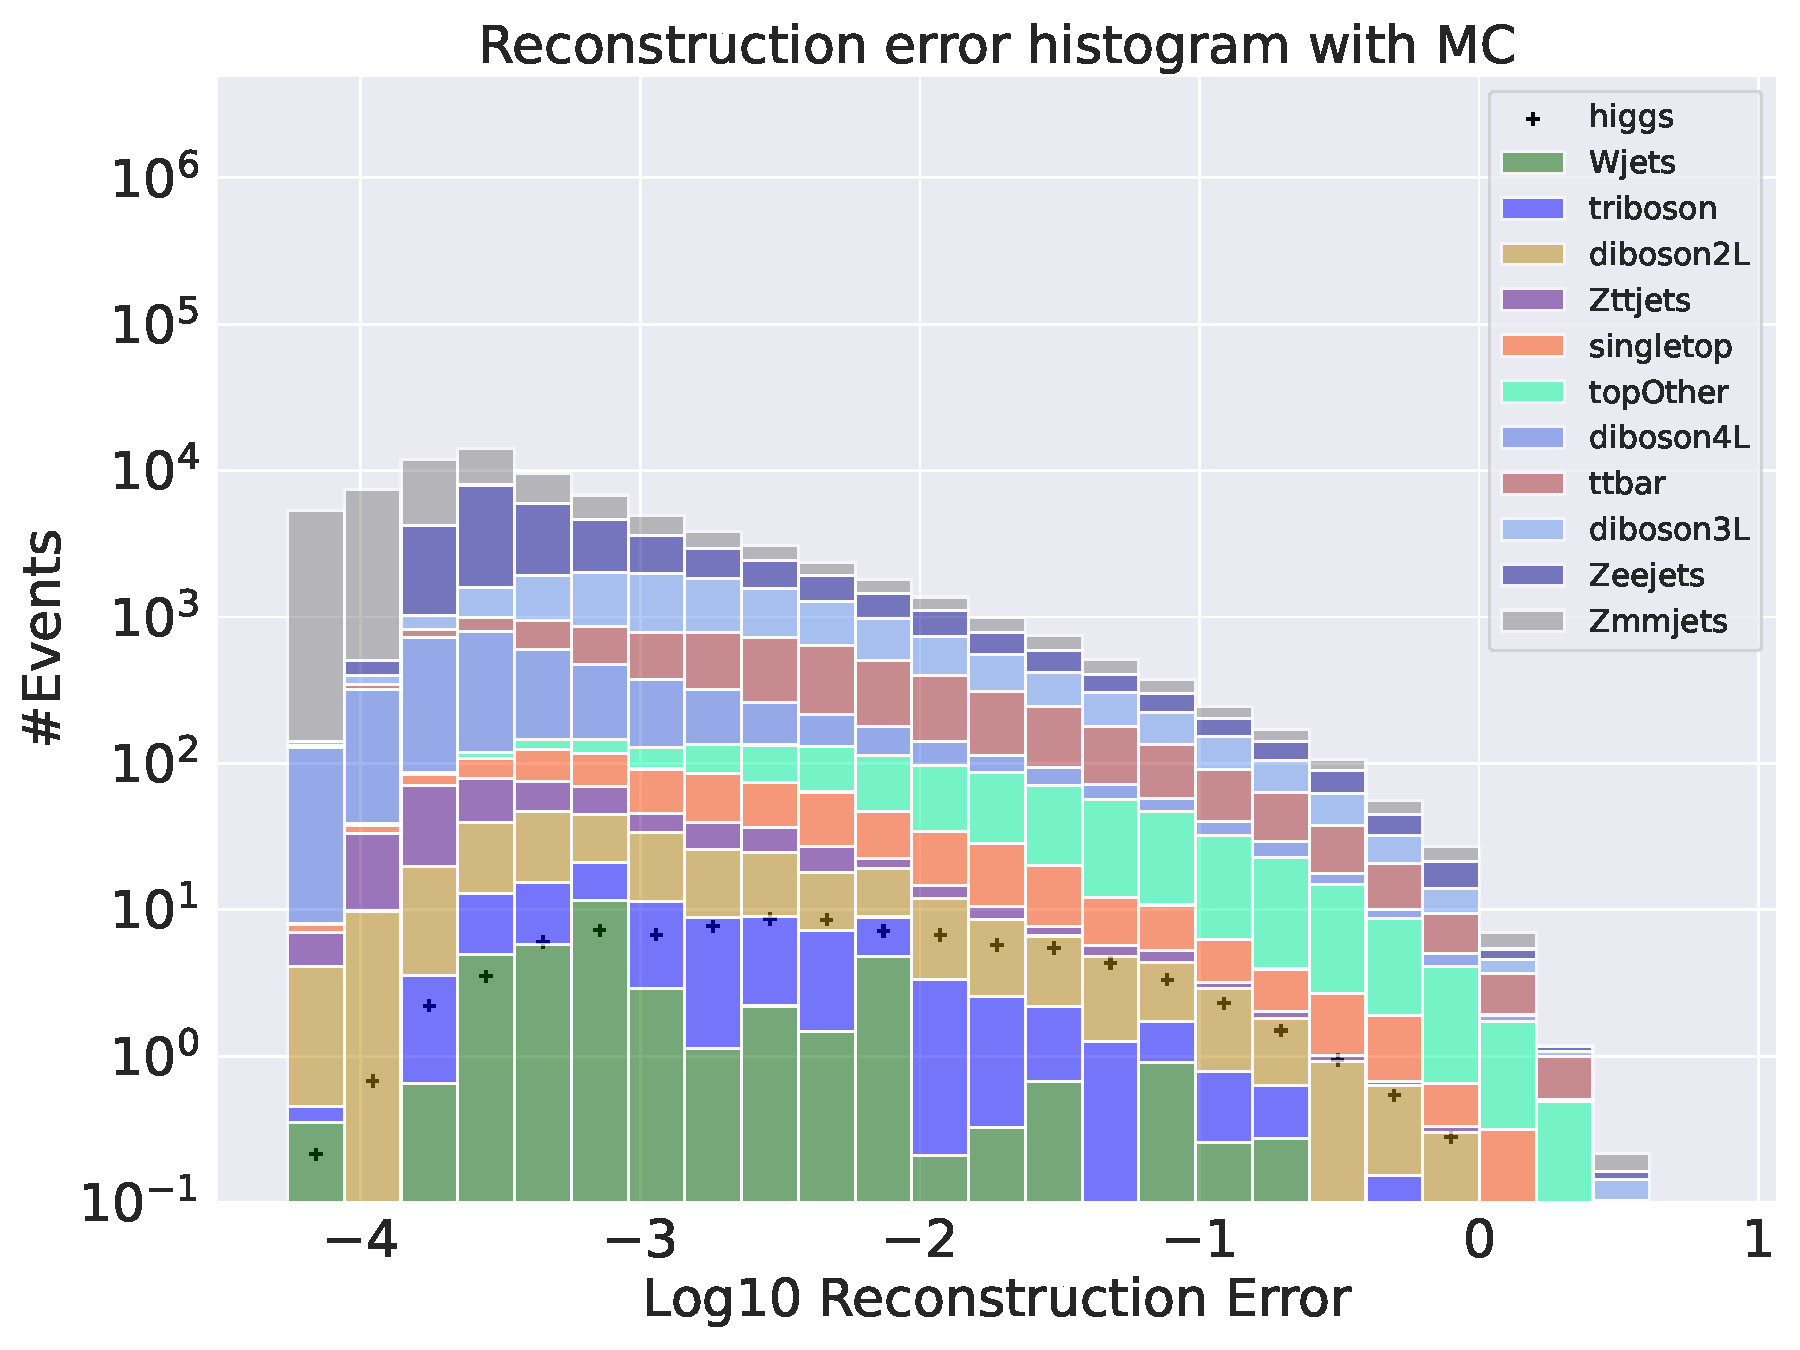
\includegraphics[width=\textwidth]{Figures/AE_testing/small/b_data_recon_big_rm3_feats_sig_higgs.pdf}
        \caption{Reconstruction error on validation SM MC from the small Autoencoder. Here the higgs channel has been removed from training and 
        is used as signal. No significant difference in distributions are found.}
        \label{fig:ae_small_higgs}
    \end{subfigure}
    \hfill 
    \begin{subfigure}{.45\textwidth}
        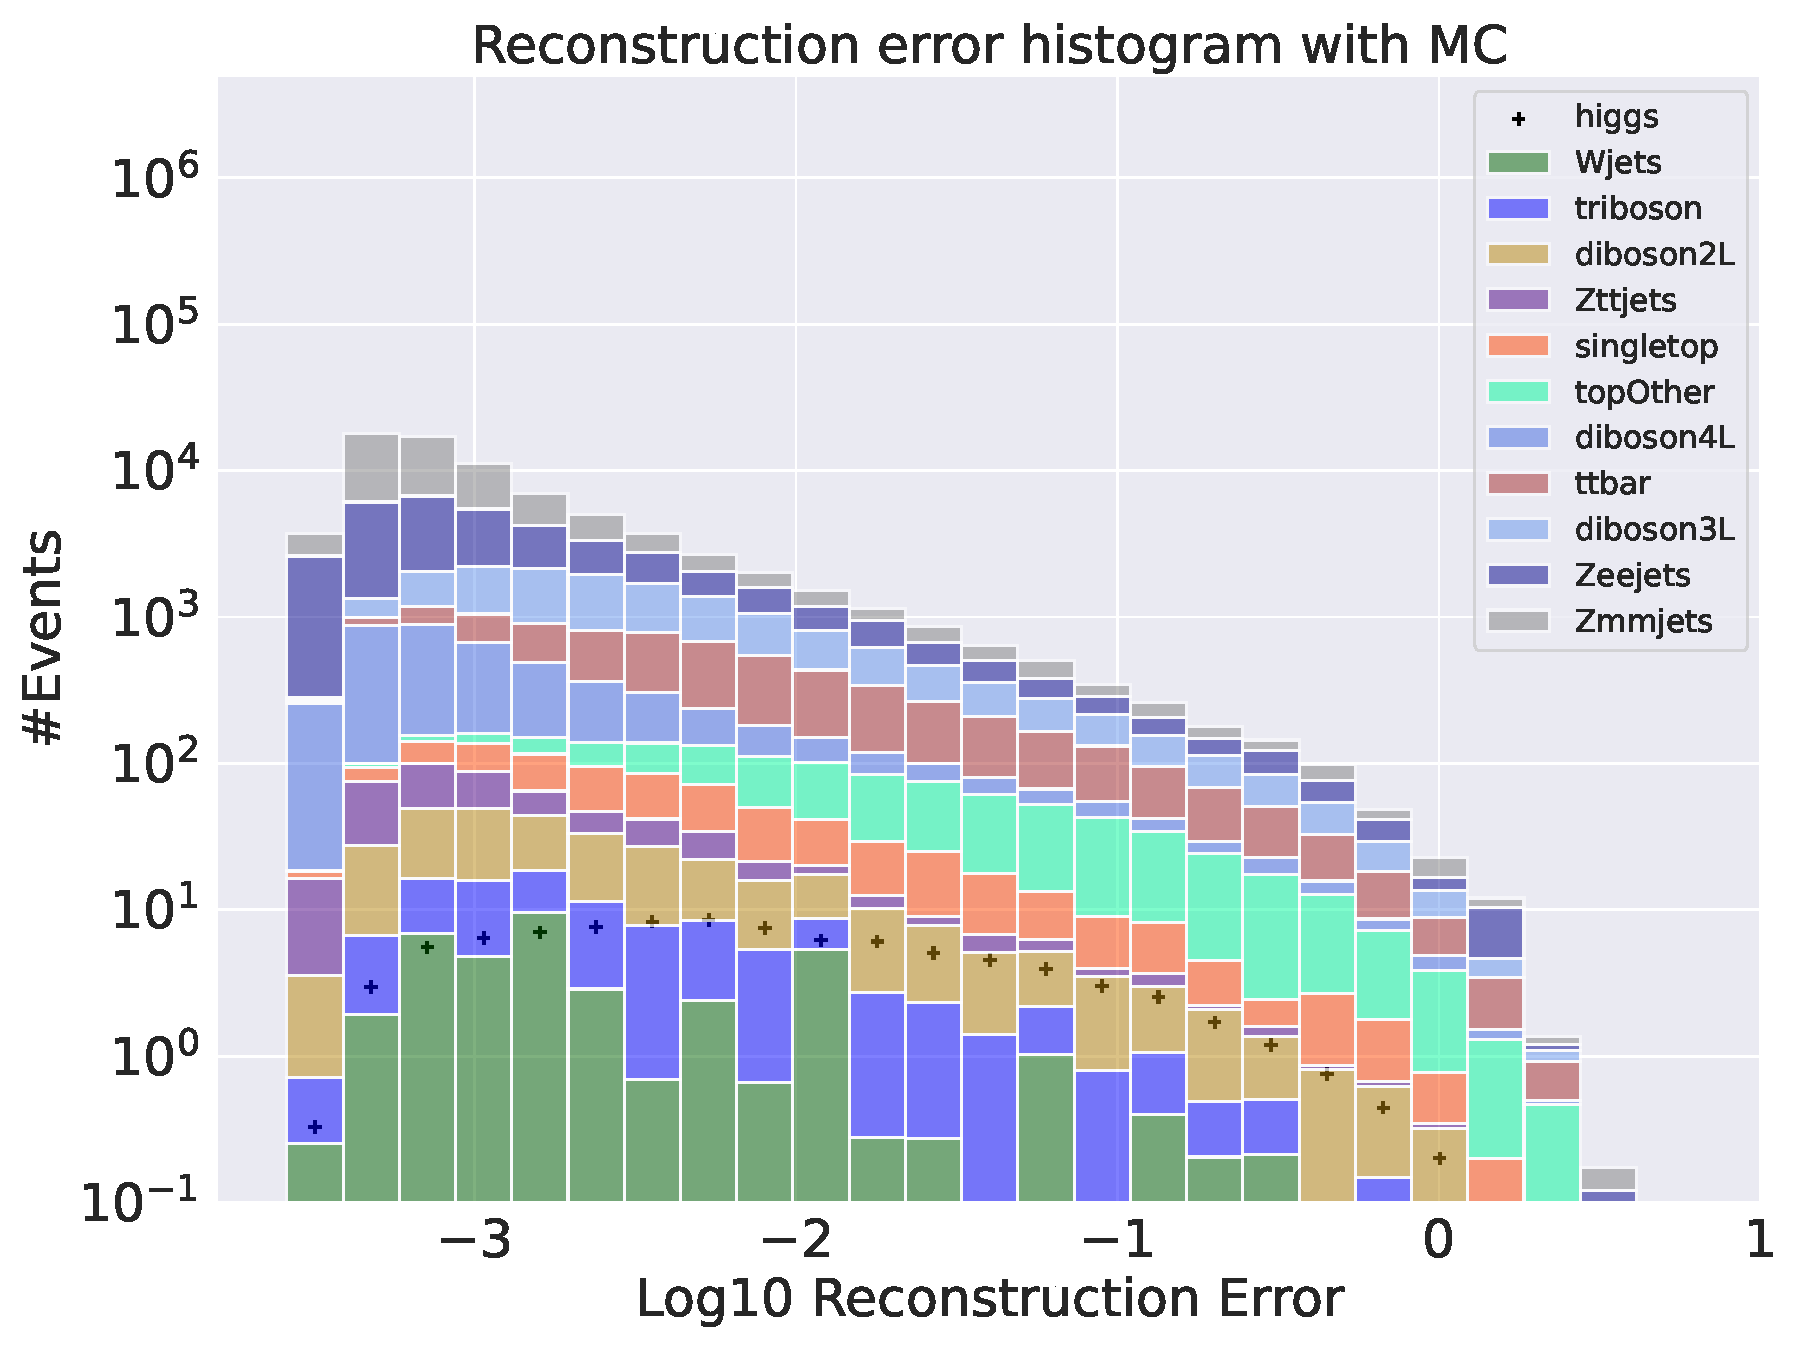
\includegraphics[width=\textwidth]{Figures/AE_testing/big/b_data_recon_big_rm3_feats_sig_higgs.pdf}
        \caption{Reconstruction error on validation SM MC from the big Autoencoder. Here the higgs channel has been removed from training and 
        is used as signal. No significant difference in distributions are found. }
        \label{fig:ae_big_higgs}
    \end{subfigure}
    \hfill  
    \label{fig:ae_big_channel_1}
\end{figure}

\begin{figure}[h!]
    \centering
    \begin{subfigure}{.45\textwidth}
        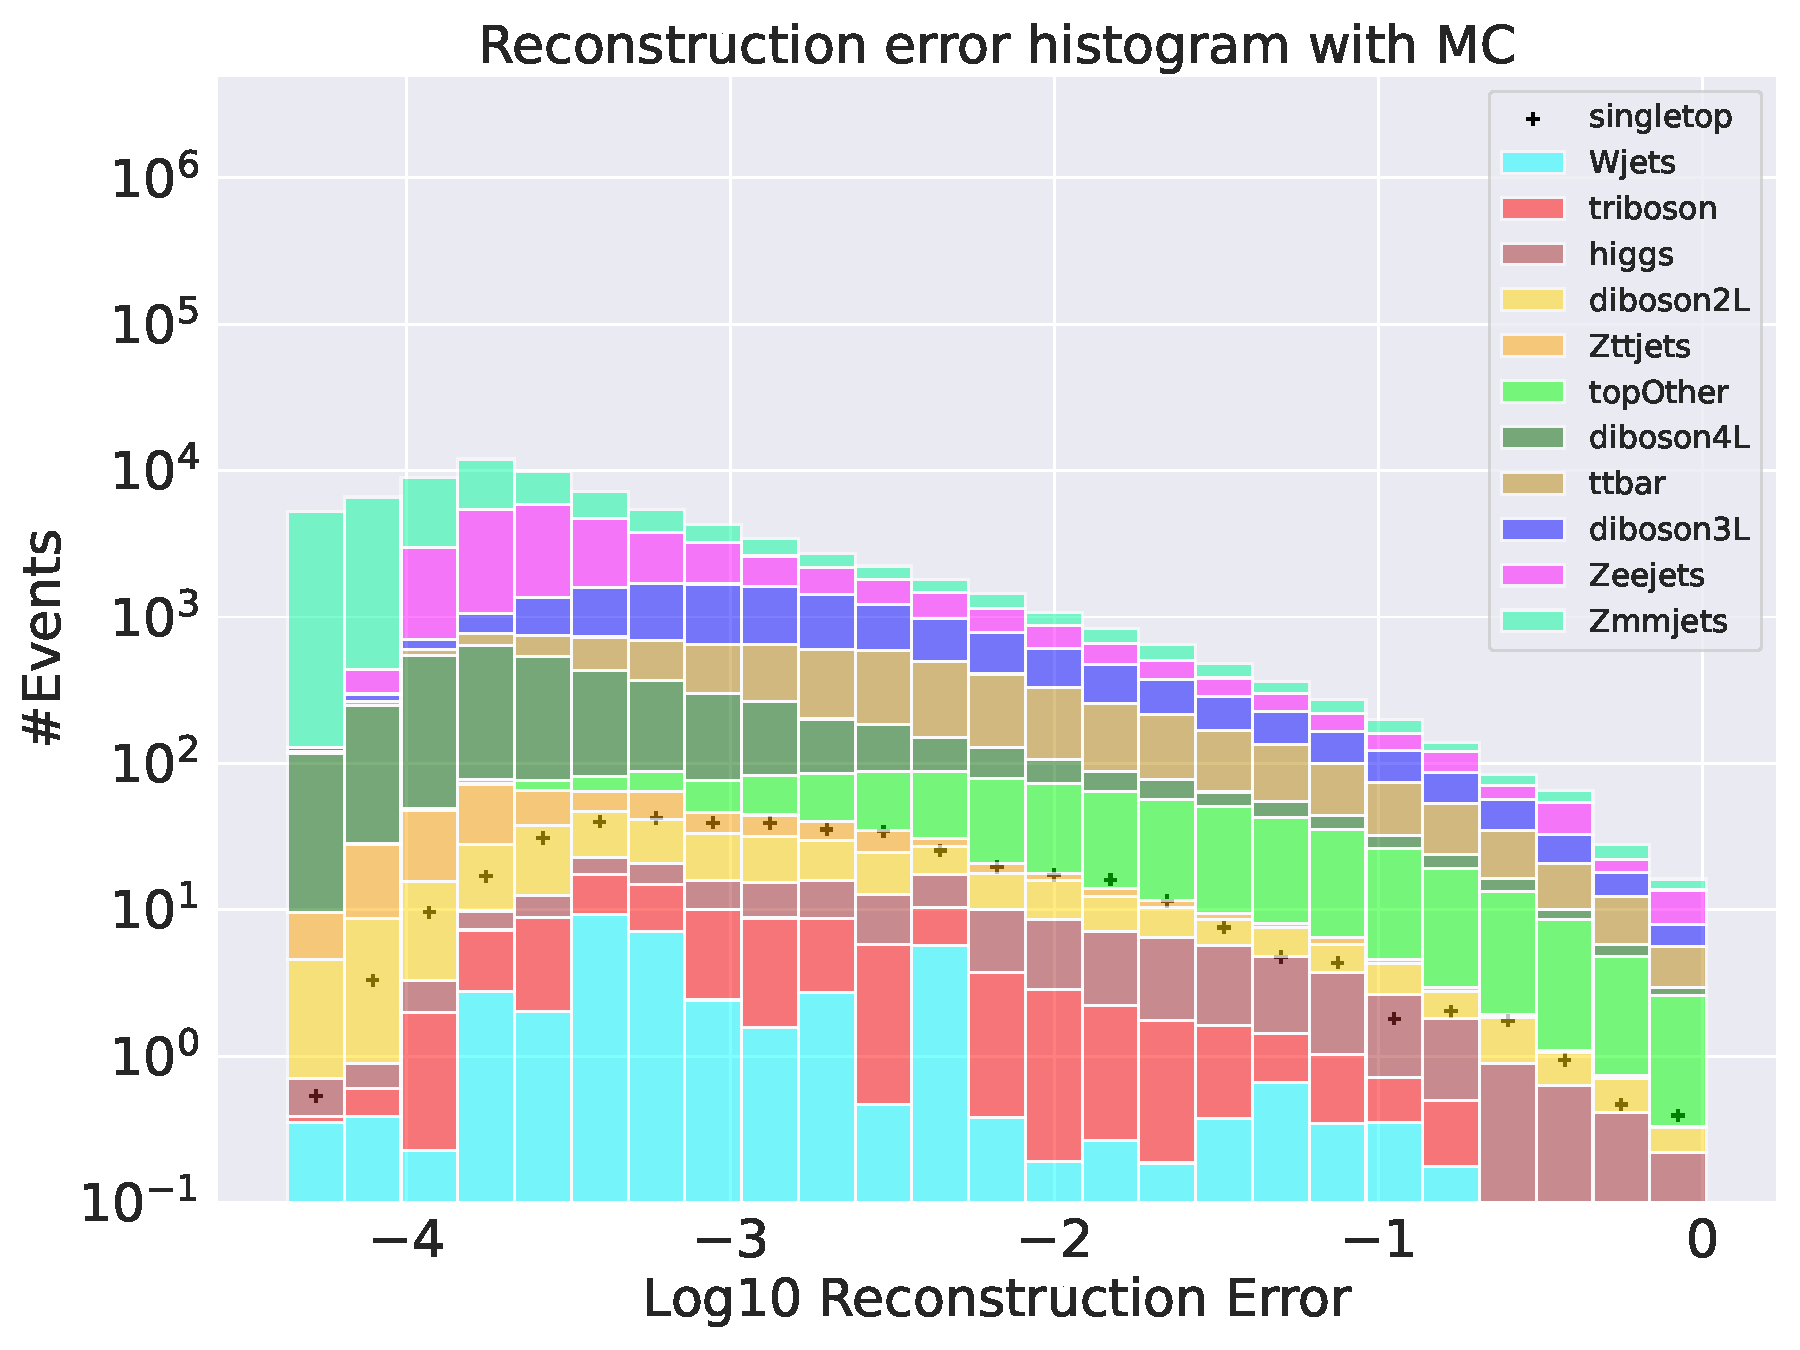
\includegraphics[width=\textwidth]{Figures/AE_testing/small/b_data_recon_big_rm3_feats_sig_singletop.pdf}
        \caption{Reconstruction error on validation SM MC from the small Autoencoder. Here the singletop channel has been removed from training and 
        is used as signal. No significant difference in distributions are found. }
        \label{fig:ae_small_singletop}
    \end{subfigure}
    \hfill
    \begin{subfigure}{.45\textwidth}
        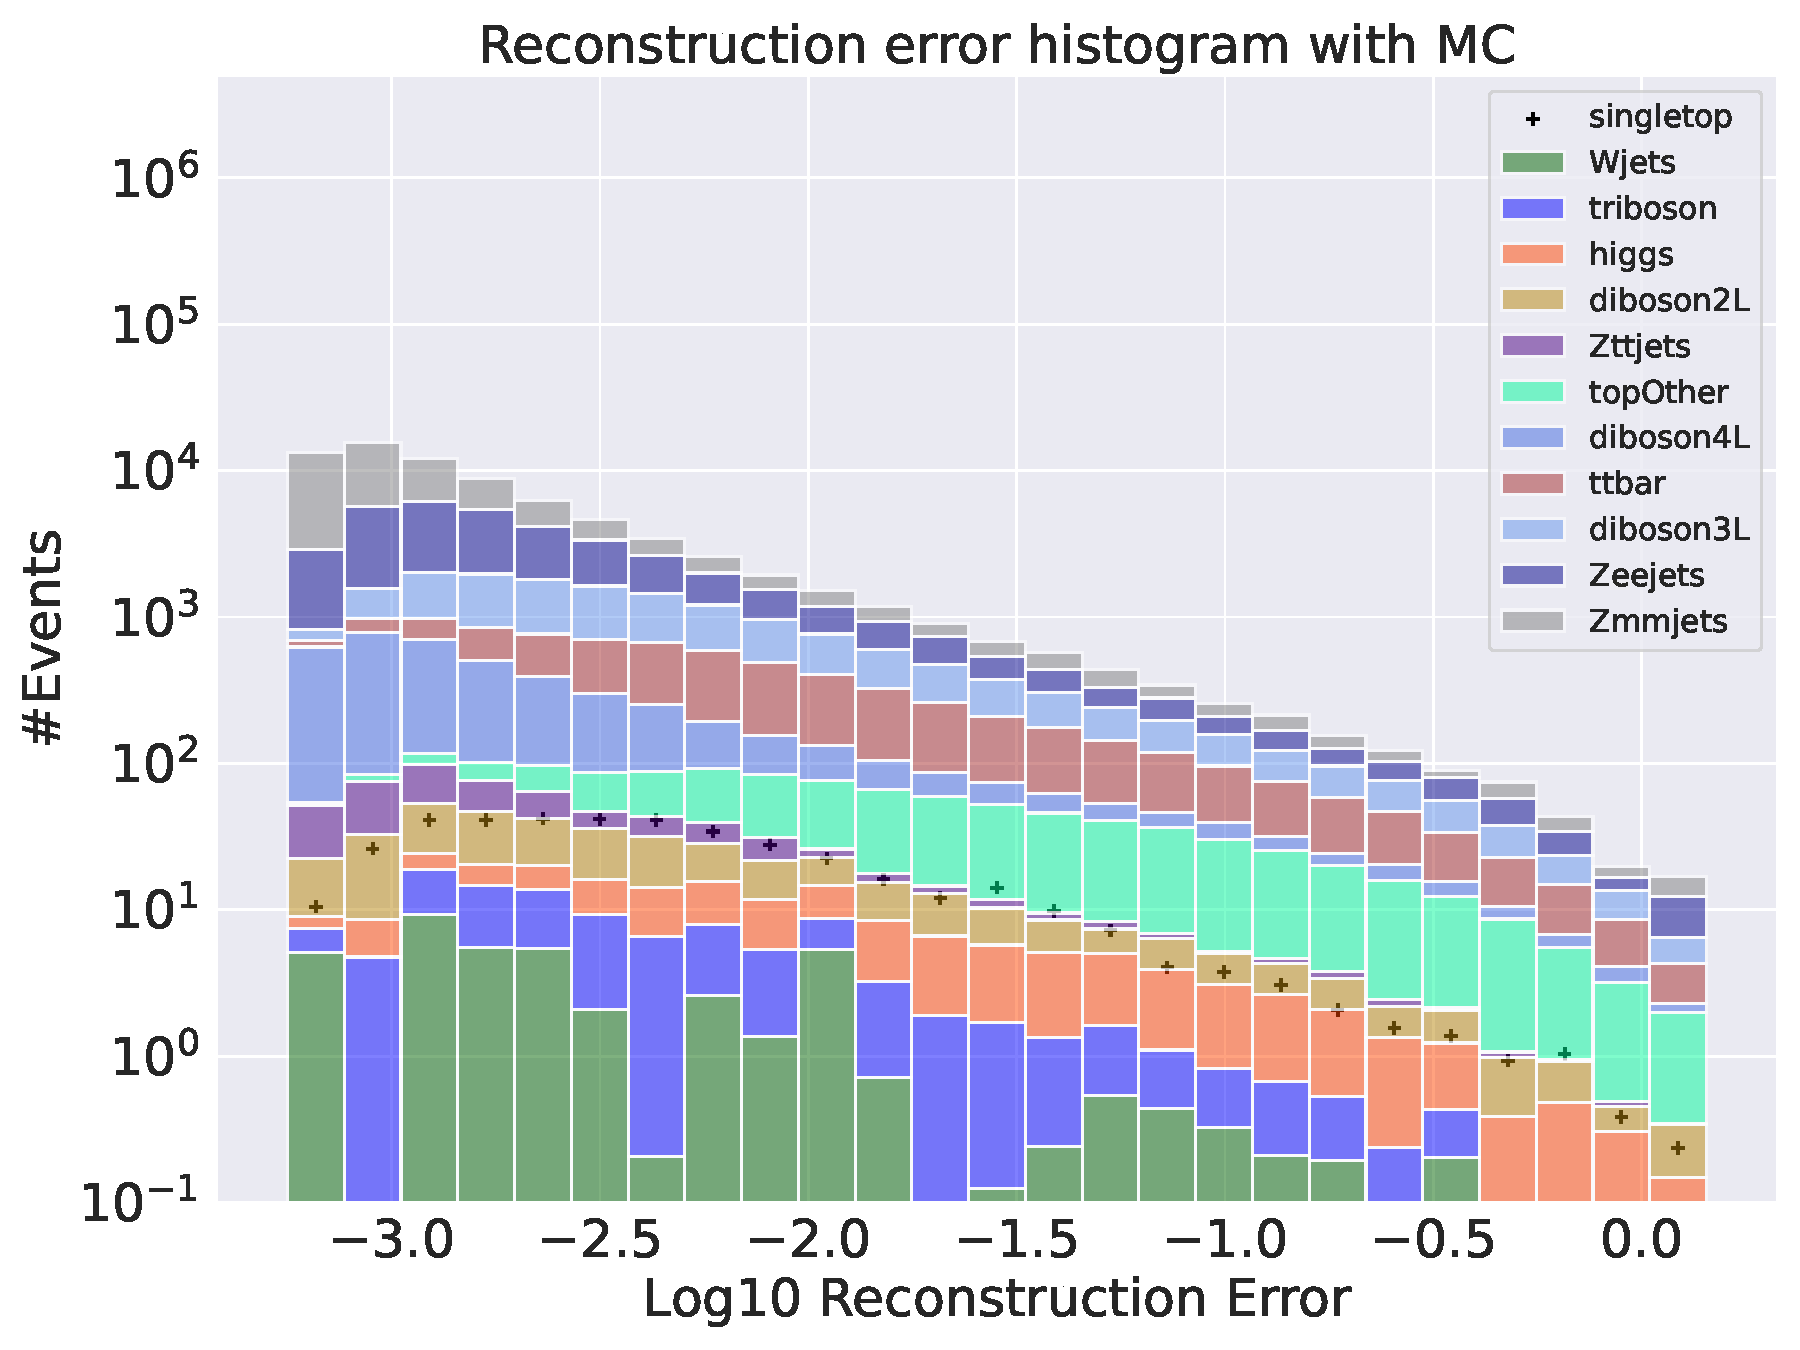
\includegraphics[width=\textwidth]{Figures/AE_testing/big/b_data_recon_big_rm3_feats_sig_singletop.pdf}
        \caption{Reconstruction error on validation SM MC from the big Autoencoder. Here the singletop channel has been removed from training and 
        is used as signal. No significant difference in distributions are found. }
        \label{fig:ae_big_singletop}
    \end{subfigure}
    \hfill 
    \label{fig:ae_big_channel_2}
\end{figure}

\begin{figure}[h!]
    \centering
    \begin{subfigure}{.45\textwidth}
        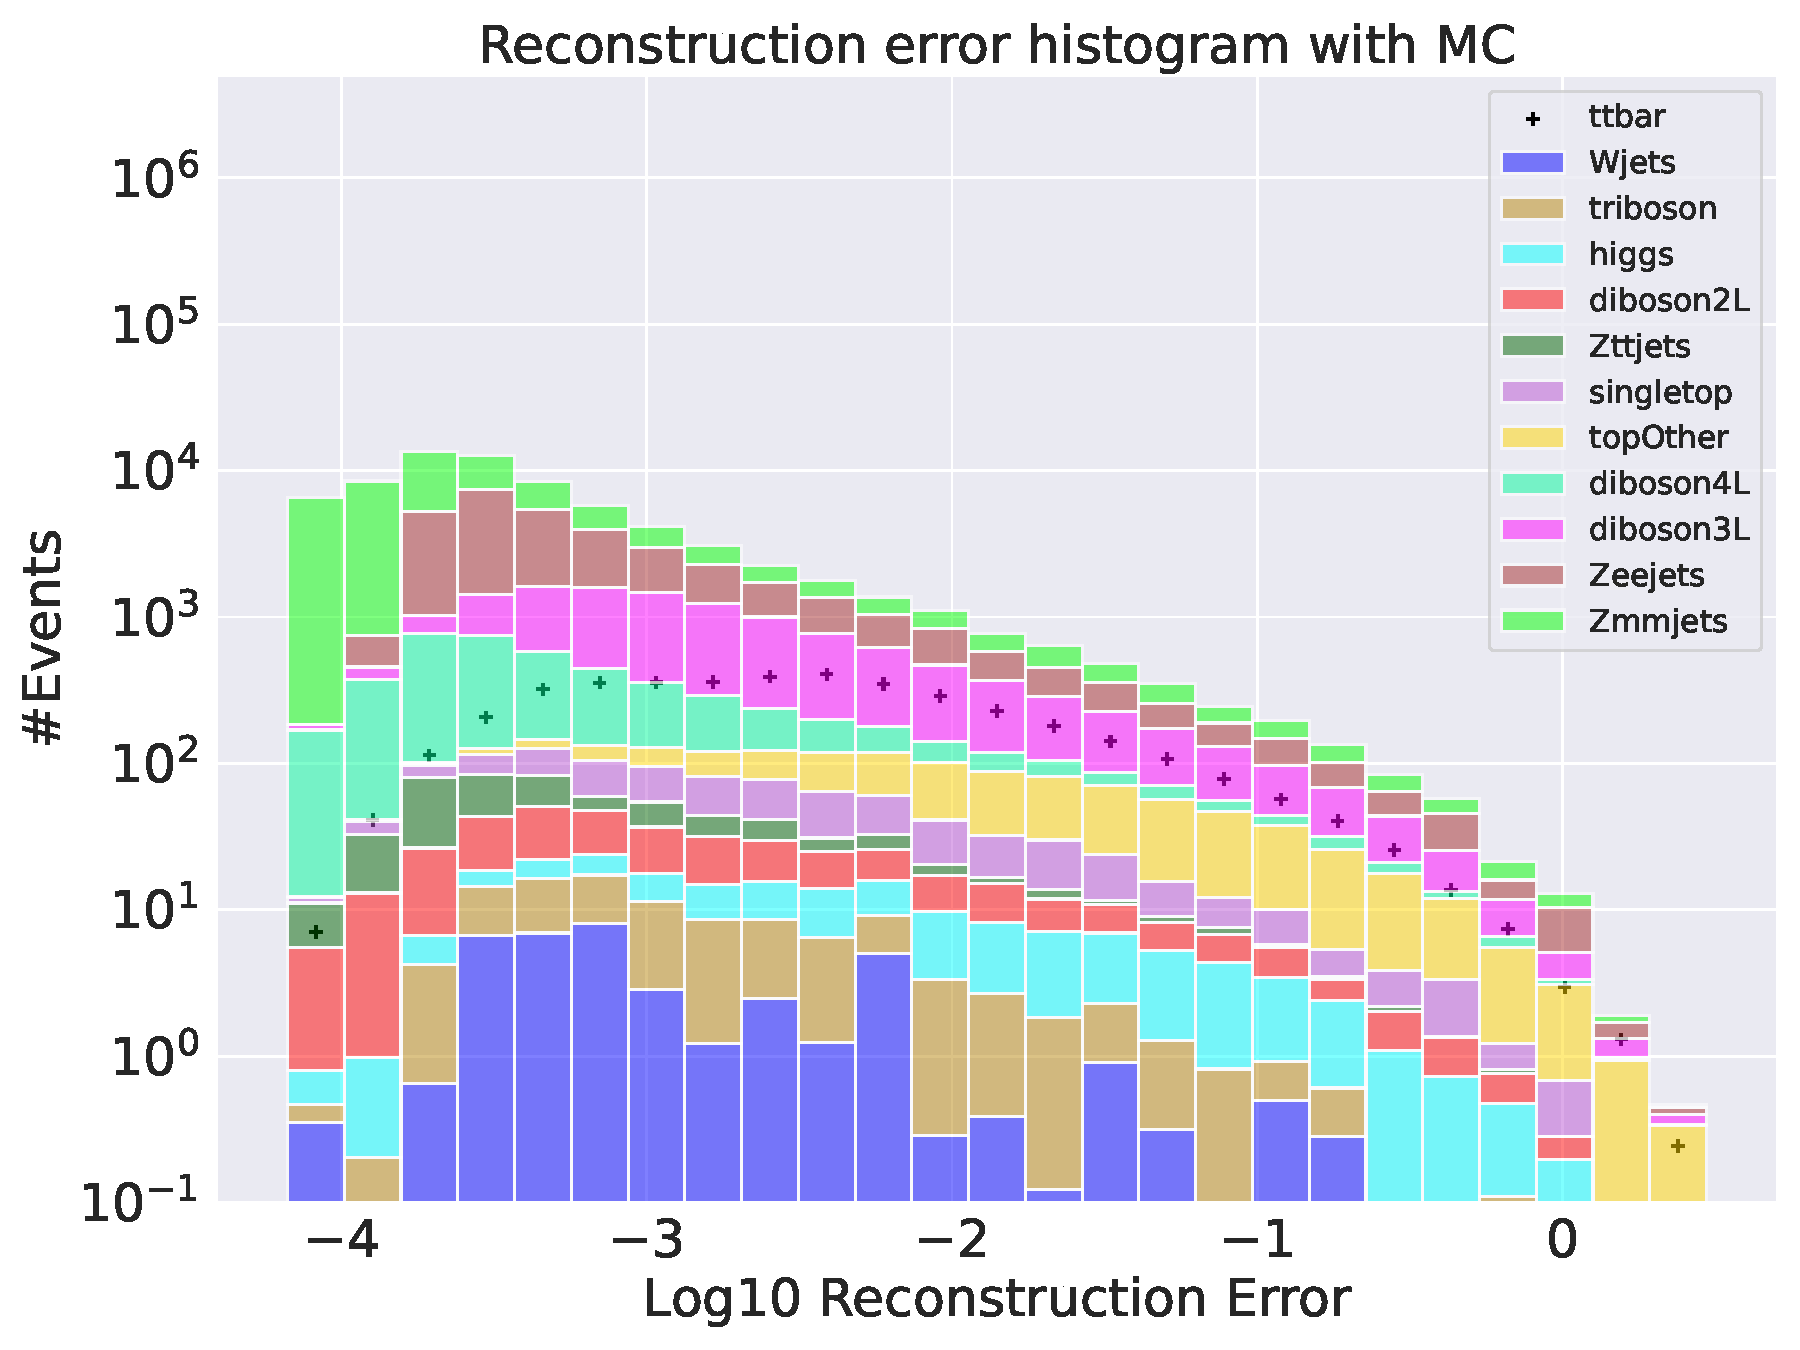
\includegraphics[width=\textwidth]{Figures/AE_testing/small/b_data_recon_big_rm3_feats_sig_ttbar.pdf}
        \caption{Reconstruction error on validation SM MC from the small Autoencoder. Here the ttbar channel has been removed from training and 
        is used as signal. No significant difference in distributions are found. }
        \label{fig:ae_small_ttbar}
    \end{subfigure}
    \hfill 
    \begin{subfigure}{.45\textwidth}
        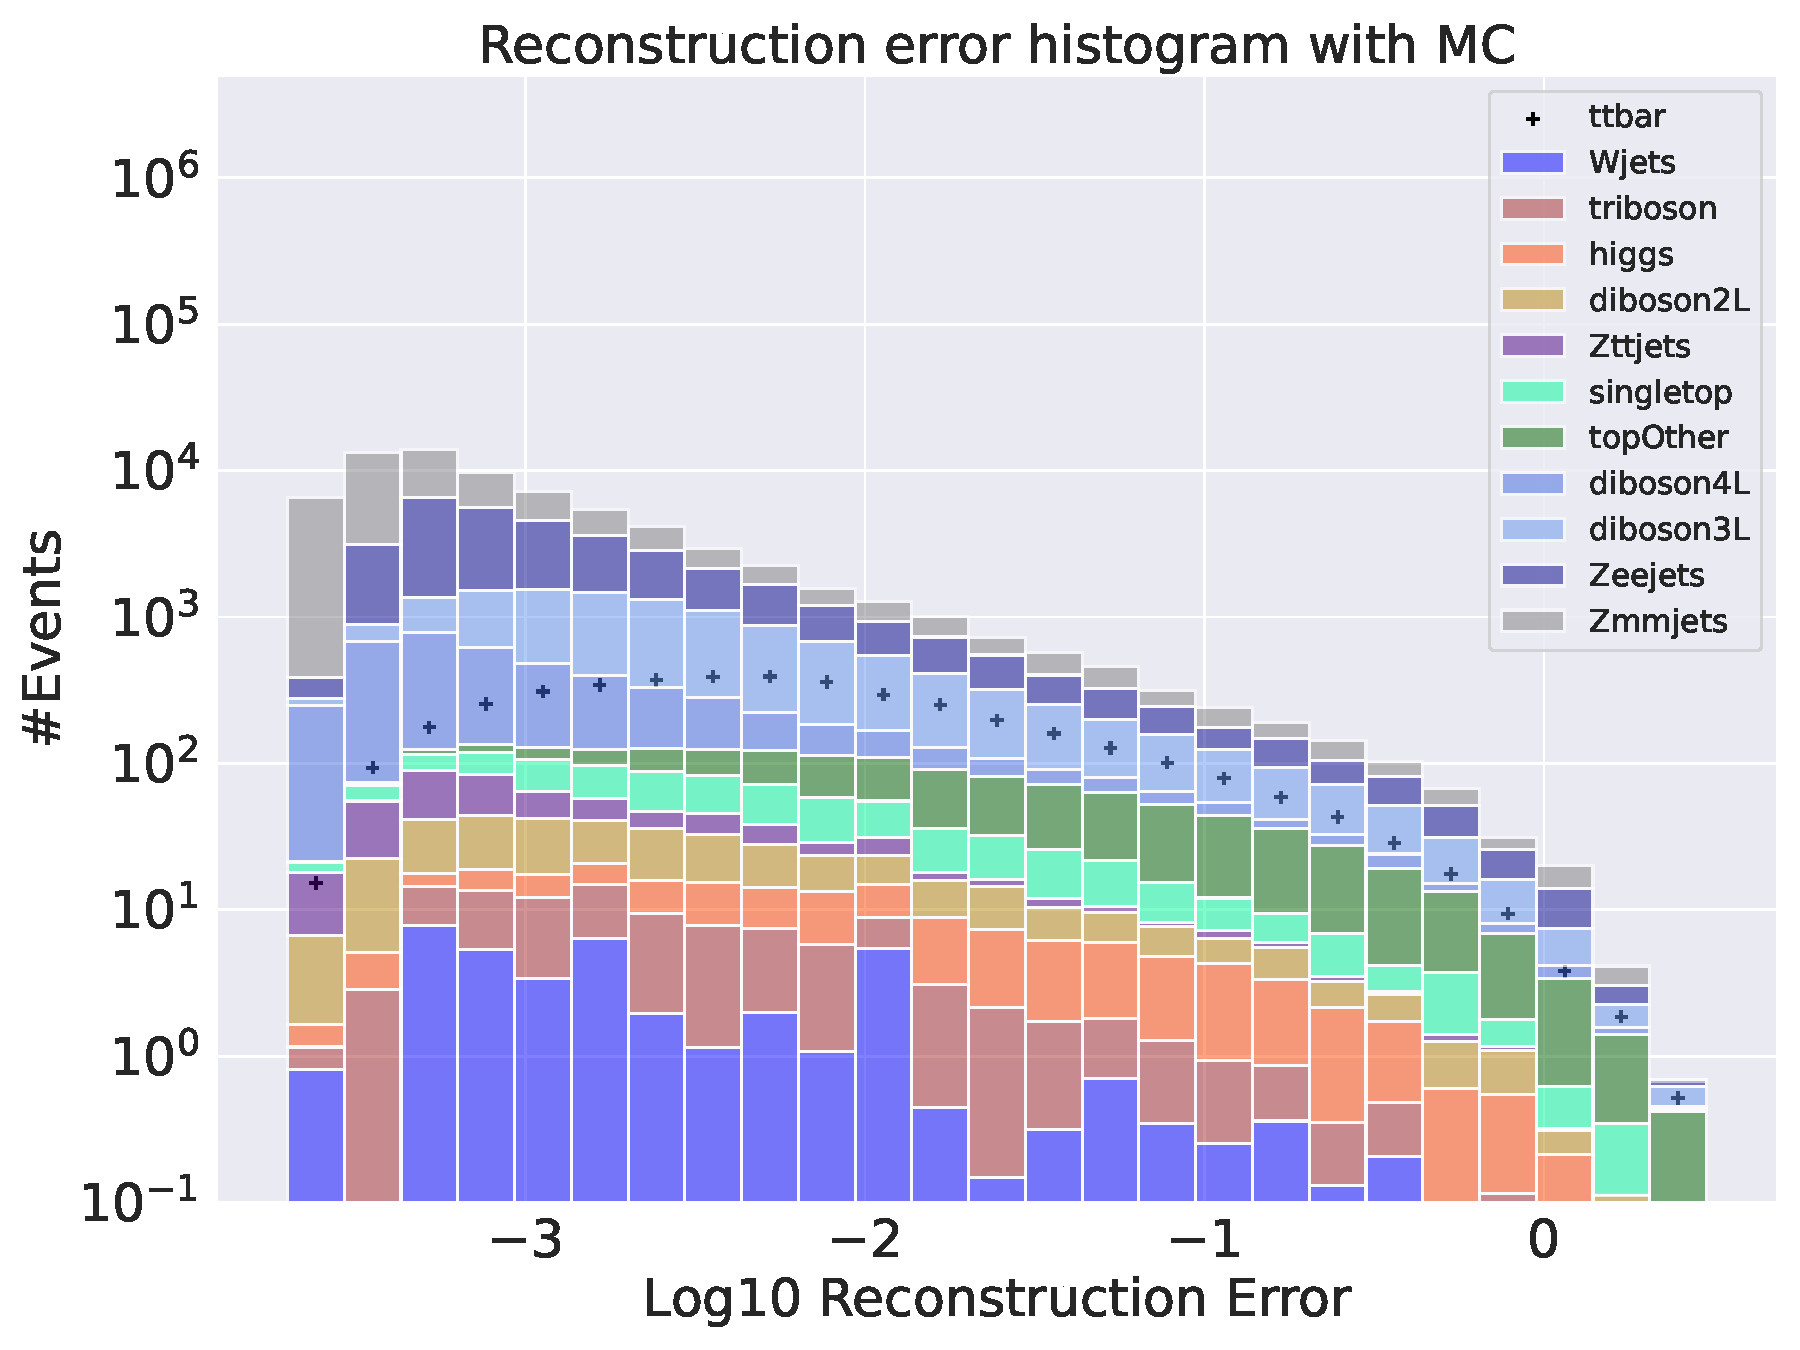
\includegraphics[width=\textwidth]{Figures/AE_testing/big/b_data_recon_big_rm3_feats_sig_ttbar.pdf}
        \caption{Reconstruction error on validation SM MC from the big Autoencoder. Here the ttbar channel has been removed from training and 
        is used as signal. No significant difference in distributions are found. }
        \label{fig:ae_big_ttbar}
    \end{subfigure}
    \hfill 
    \label{fig:ae_big_channel_3}
\end{figure}



\subsubsection*{Variational Autoencoder}
Both the large and small autoencoder produced results, and are shown below. The small autoencoder results will always be first for each of the tests. 


\begin{figure}[h!]
    \centering
    \begin{subfigure}{.45\textwidth}
        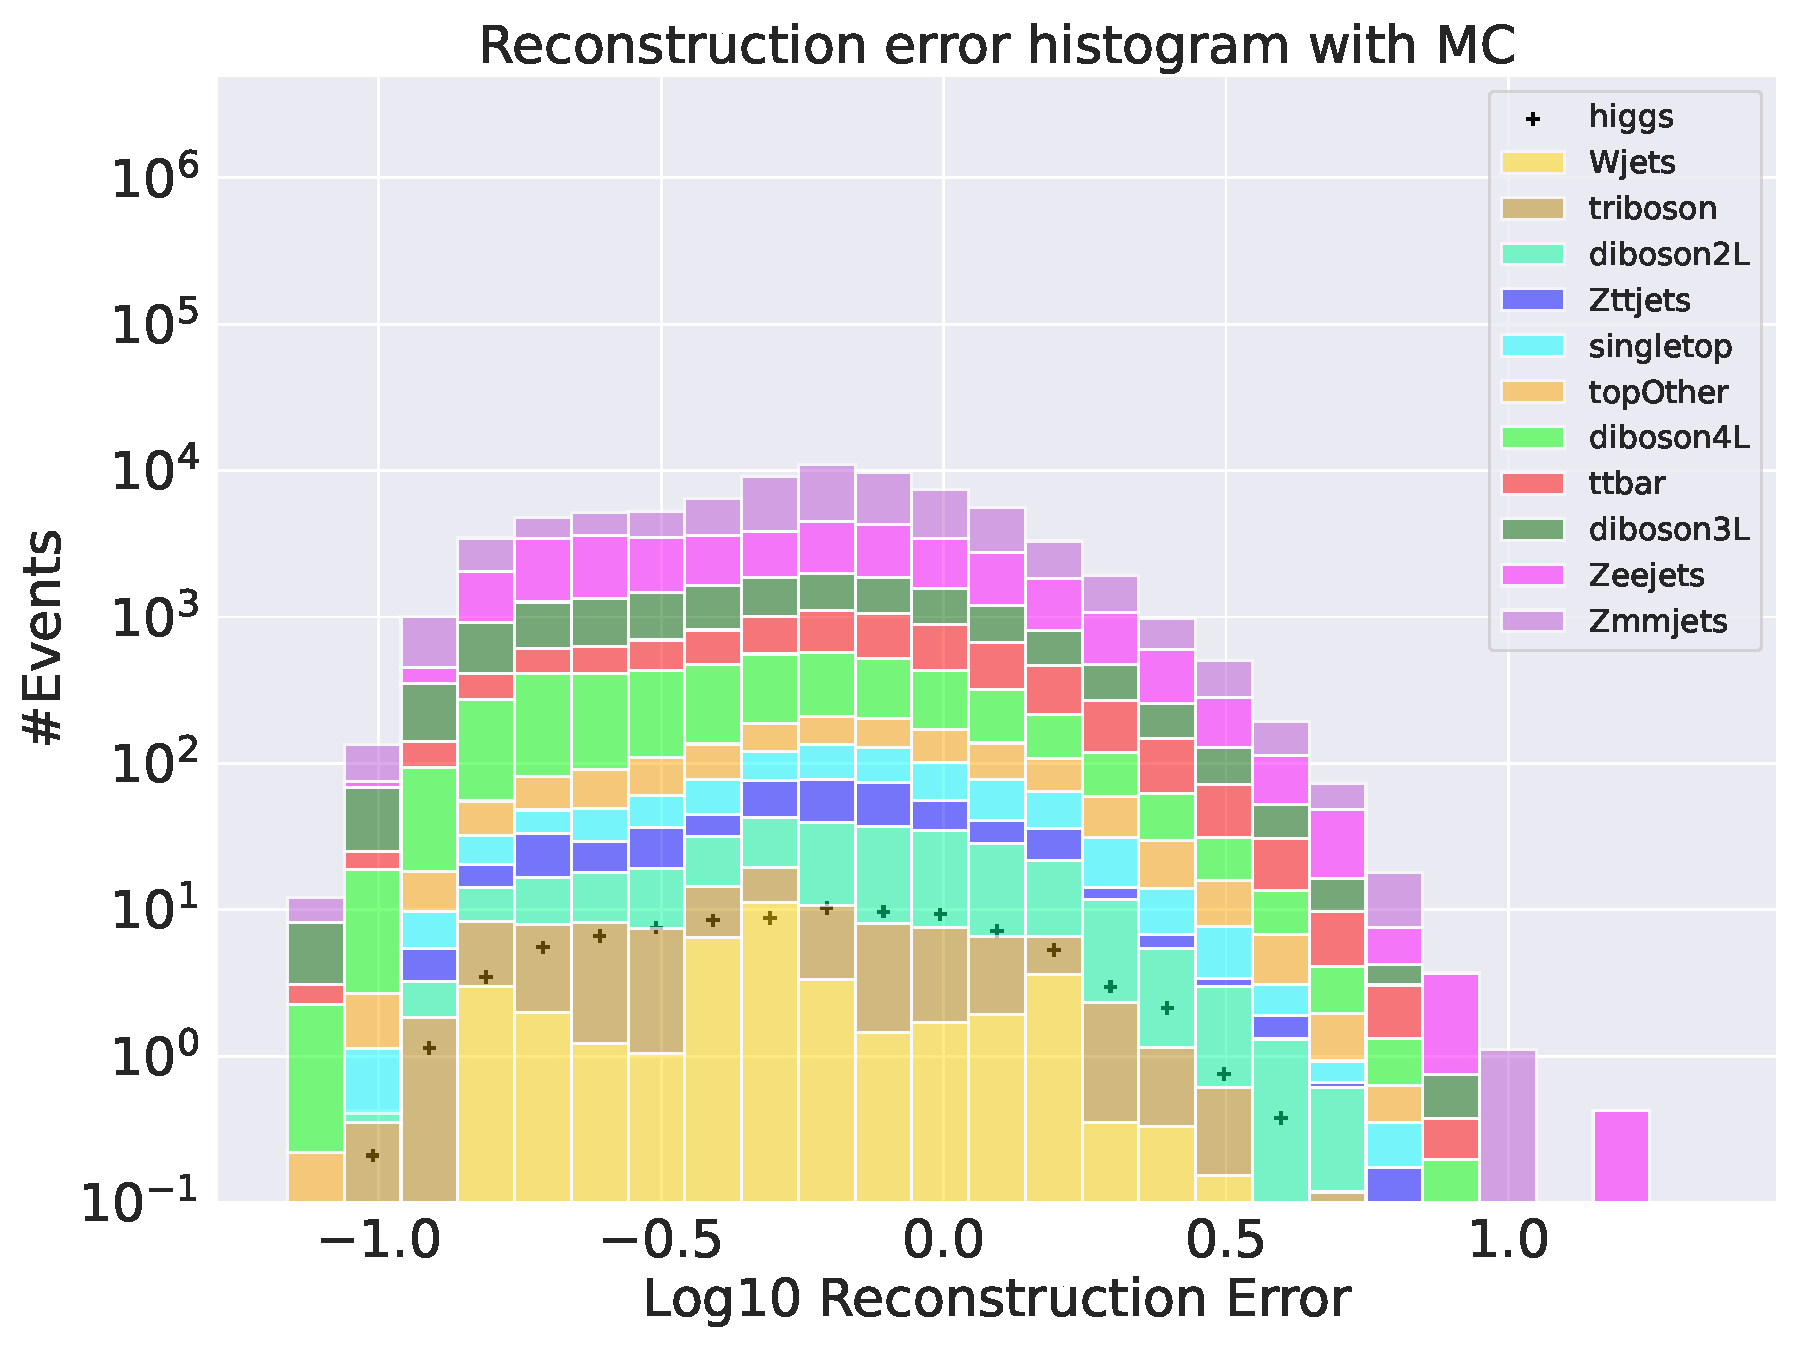
\includegraphics[width=\textwidth]{Figures/VAE_testing/small/b_data_recon_big_rm3_feats_sig_higgs.pdf}
        \caption{Reconstruction error on validation SM MC from the small variational Autoencoder. Here the higgs channel has been removed from training and 
        is used as signal. No significant difference in distributions are found.}
        \label{fig:vae_small_higgs}
    \end{subfigure}
    \hfill 
    \begin{subfigure}{.45\textwidth}
        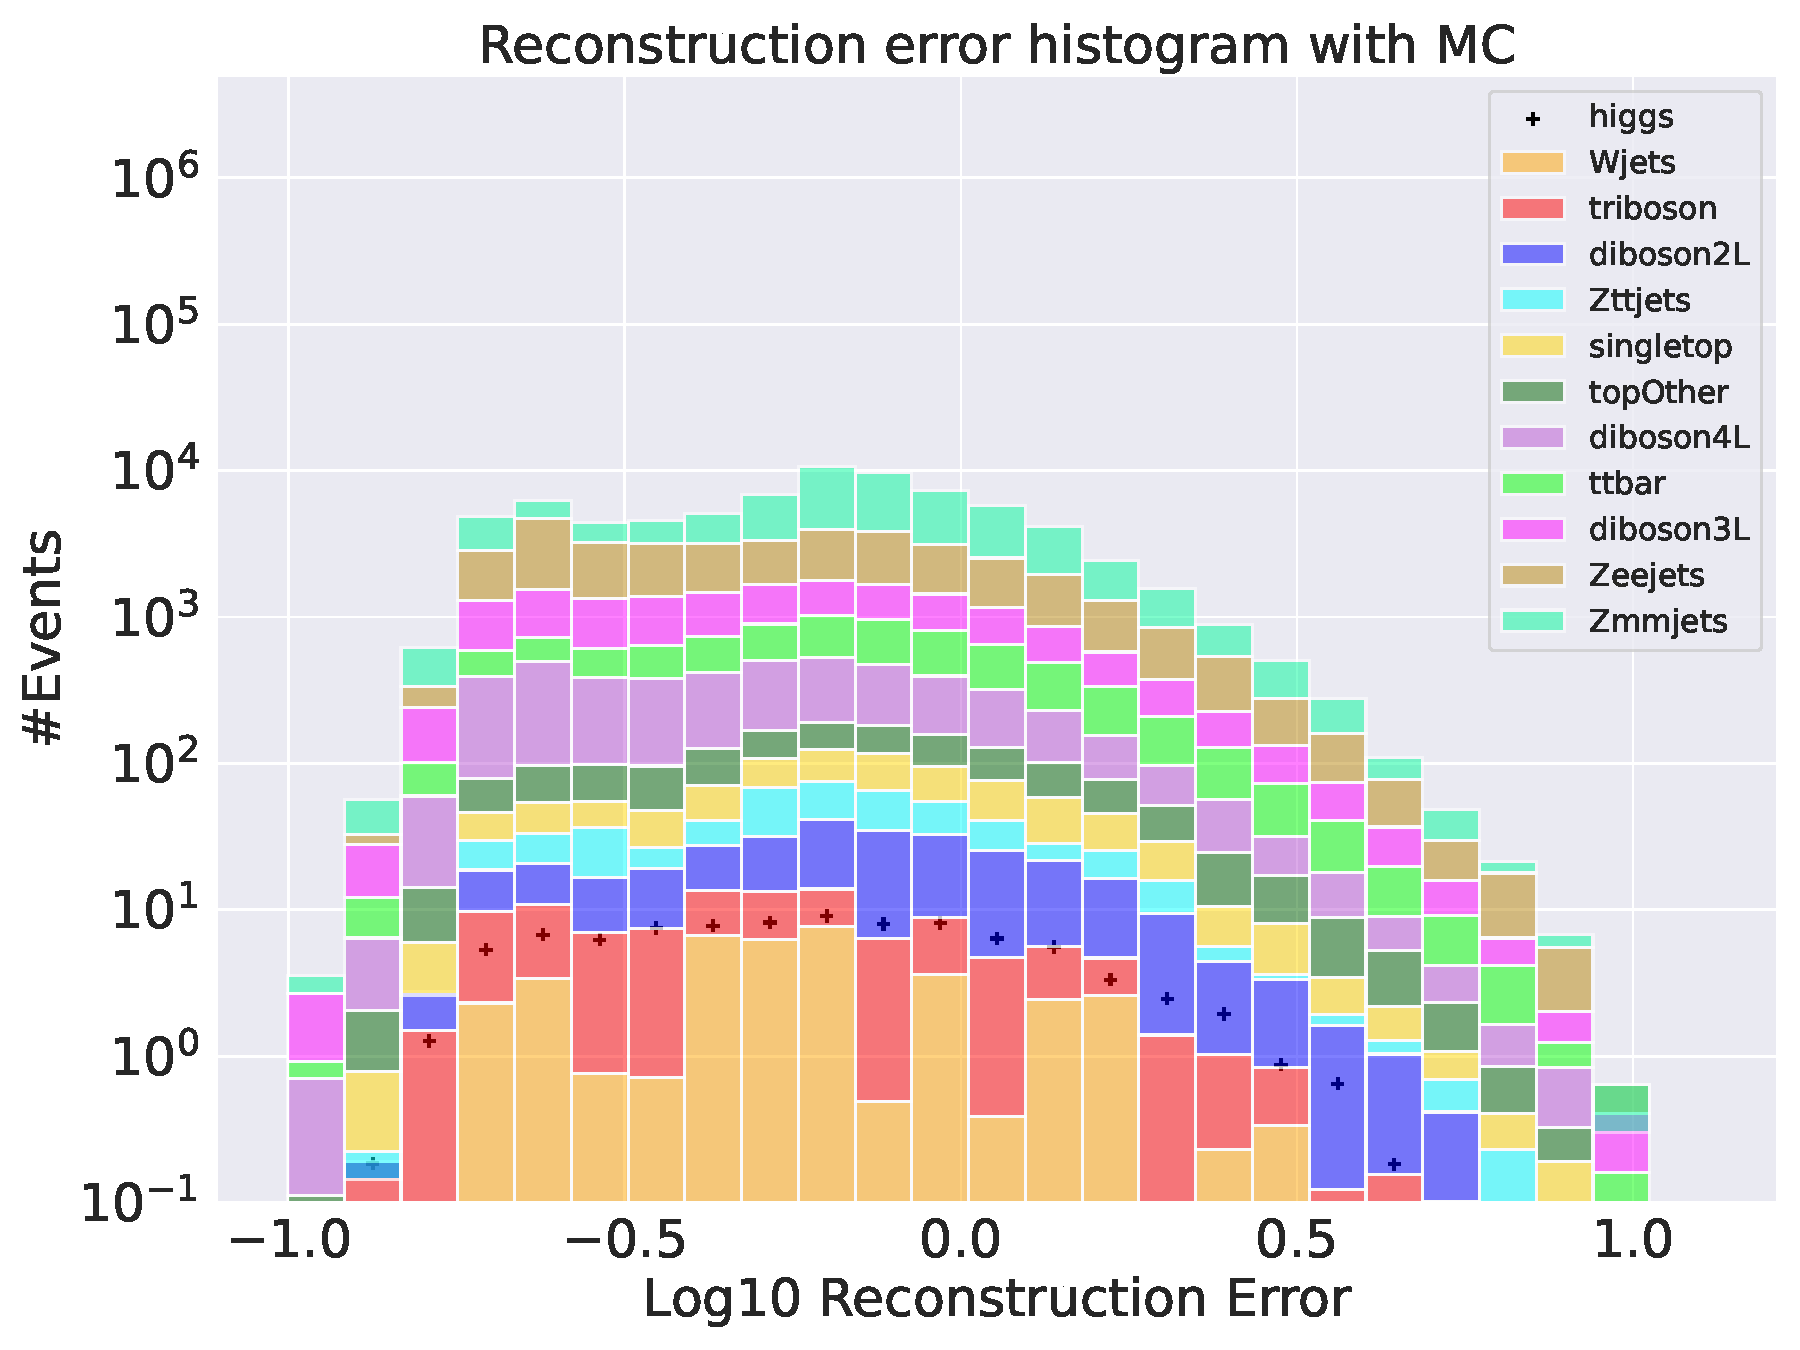
\includegraphics[width=\textwidth]{Figures/VAE_testing/big/b_data_recon_big_rm3_feats_sig_higgs.pdf}
        \caption{Reconstruction error on validation SM MC from the big variational Autoencoder. Here the higgs channel has been removed from training and 
        is used as signal. No significant difference in distributions are found. }
        \label{fig:vae_big_higgs}
    \end{subfigure}
    \hfill  
    \label{fig:vae_big_channel_1}
\end{figure}

\begin{figure}[h!]
    \centering
    \begin{subfigure}{.45\textwidth}
        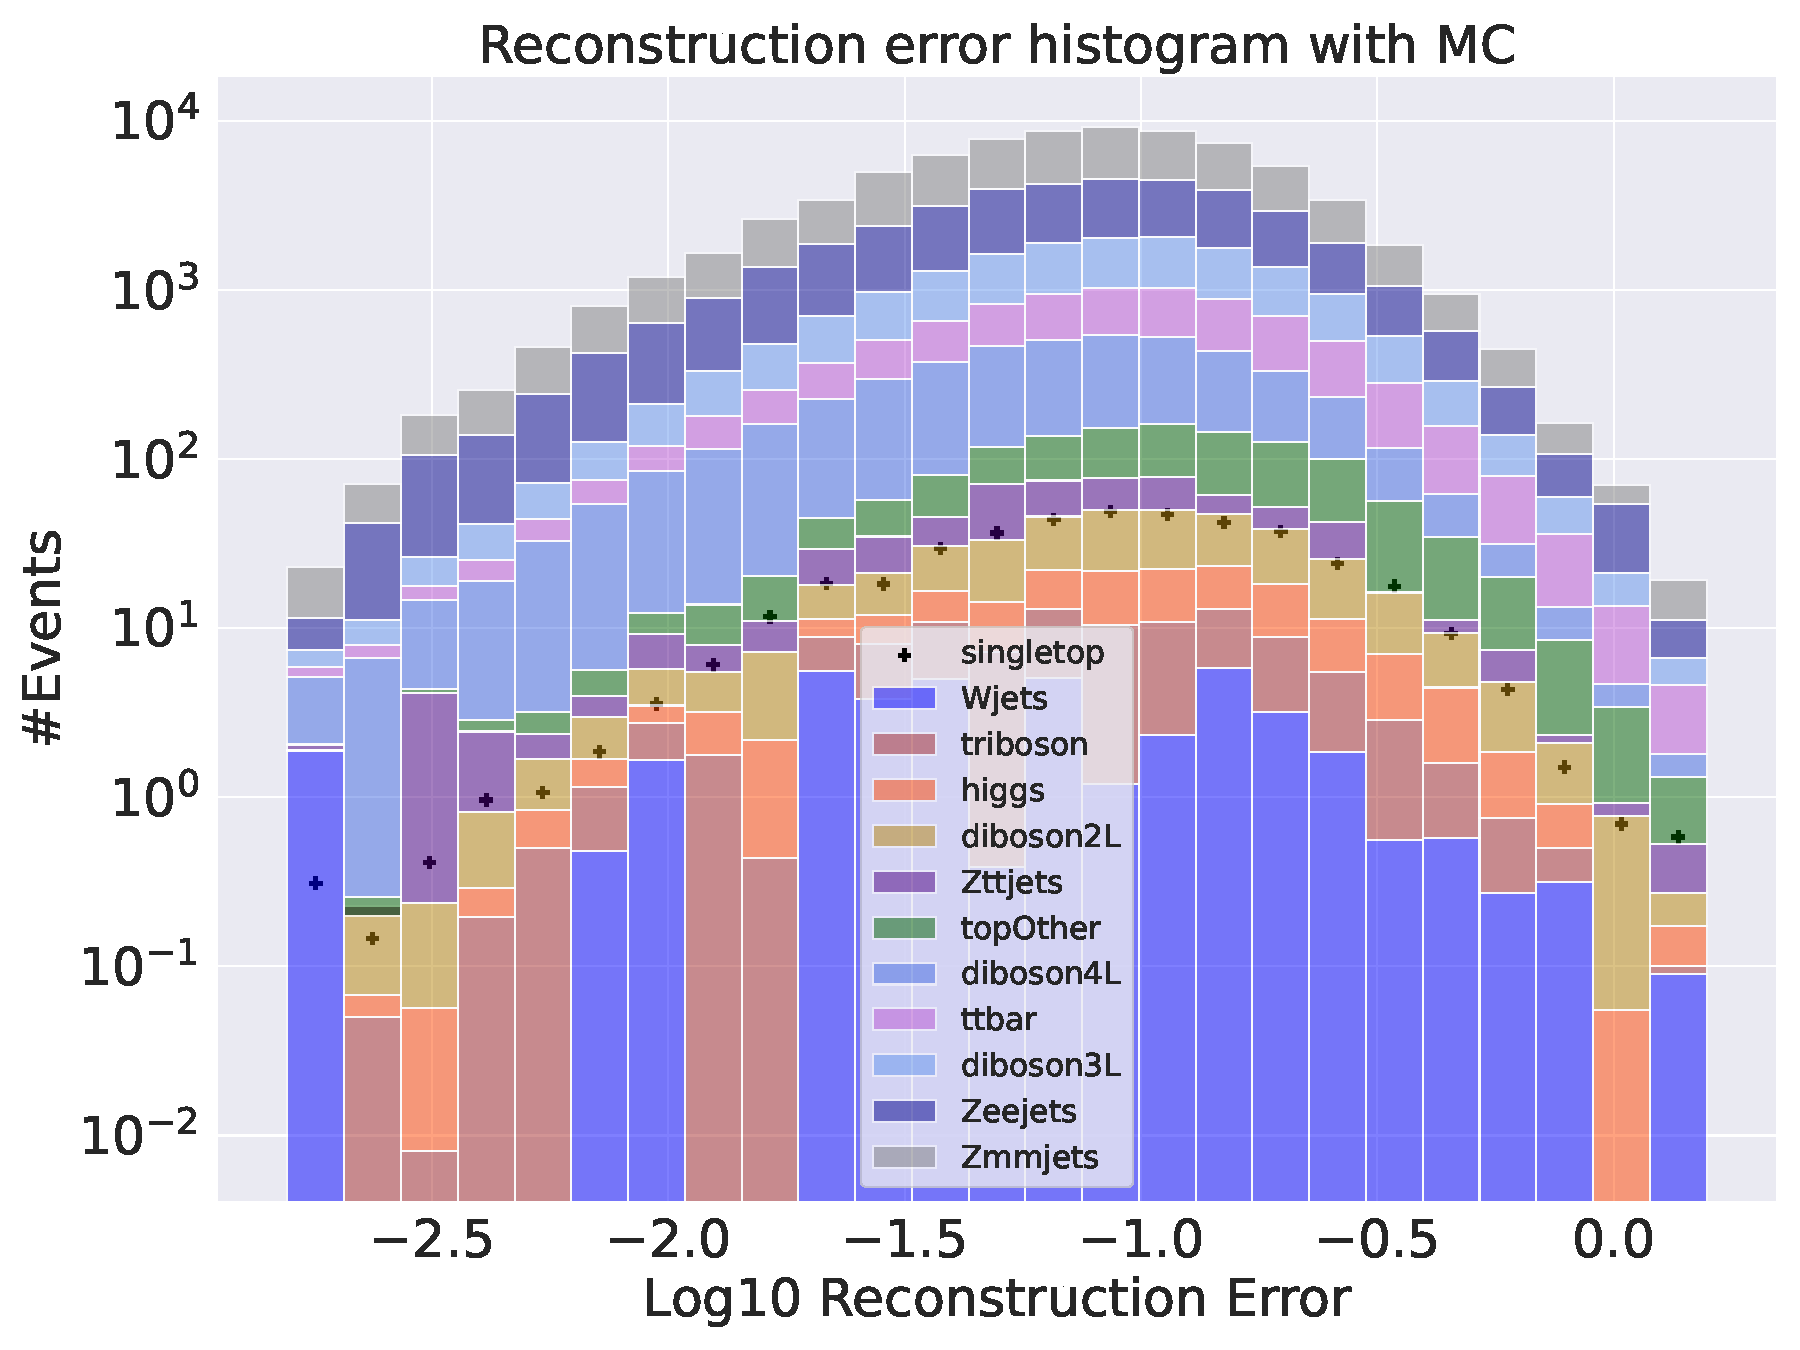
\includegraphics[width=\textwidth]{Figures/VAE_testing/small/b_data_recon_big_rm3_feats_sig_singletop.pdf}
        \caption{Reconstruction error on validation SM MC from the small variational Autoencoder. Here the singletop channel has been removed from training and 
        is used as signal. No significant difference in distributions are found. }
        \label{fig:vae_small_singletop}
    \end{subfigure}
    \hfill
    \begin{subfigure}{.45\textwidth}
        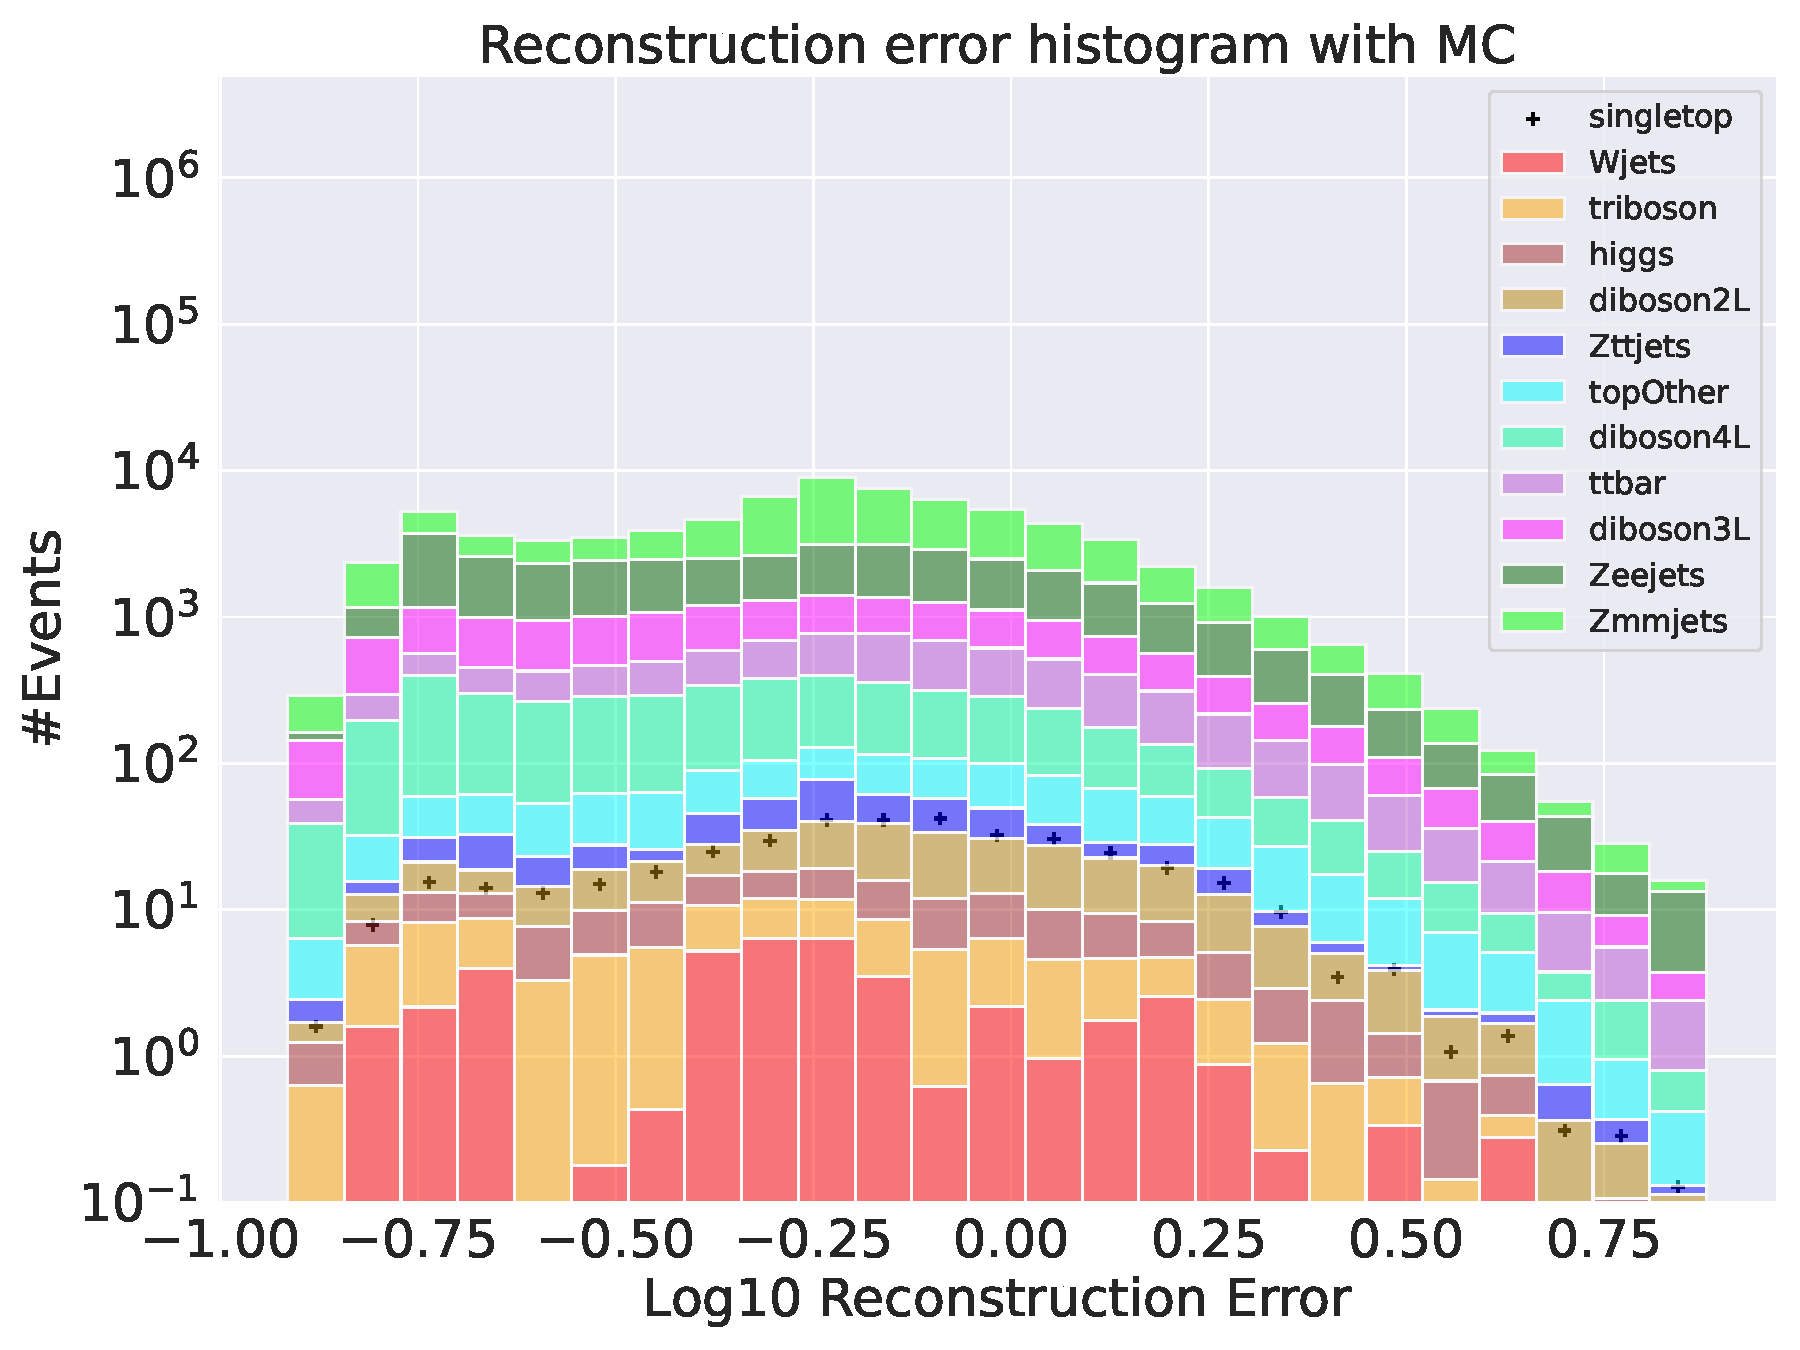
\includegraphics[width=\textwidth]{Figures/VAE_testing/big/b_data_recon_big_rm3_feats_sig_singletop.pdf}
        \caption{Reconstruction error on validation SM MC from the big variational Autoencoder. Here the singletop channel has been removed from training and 
        is used as signal. No significant difference in distributions are found. }
        \label{fig:vae_big_singletop}
    \end{subfigure}
    \hfill 
    \label{fig:vae_big_channel_2}
\end{figure}

\begin{figure}[h!]
    \centering
    \begin{subfigure}{.45\textwidth}
        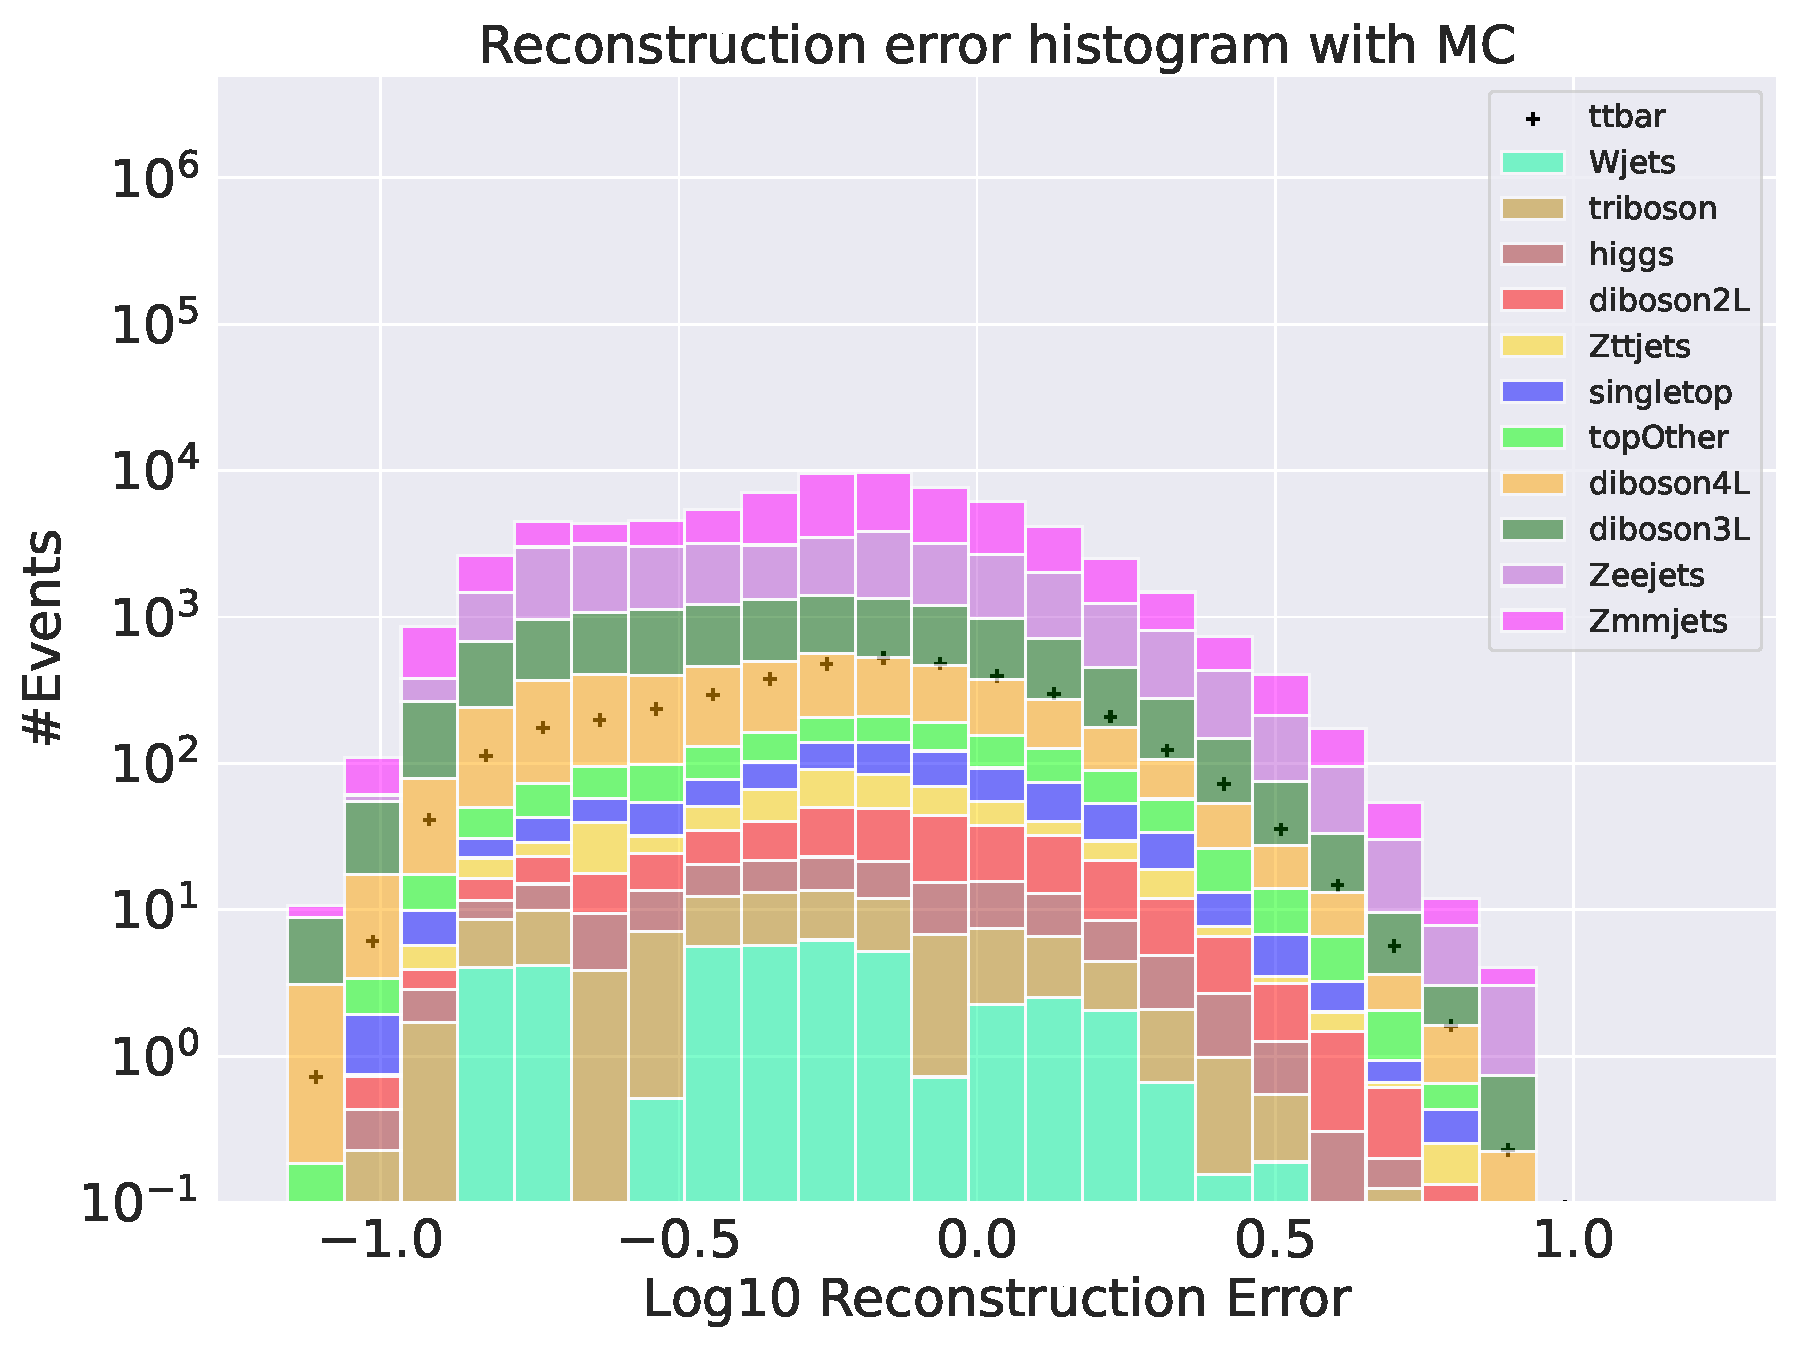
\includegraphics[width=\textwidth]{Figures/VAE_testing/small/b_data_recon_big_rm3_feats_sig_ttbar.pdf}
        \caption{Reconstruction error on validation SM MC from the small variational Autoencoder. Here the ttbar channel has been removed from training and 
        is used as signal. No significant difference in distributions are found. }
        \label{fig:vae_small_ttbar}
    \end{subfigure}
    \hfill 
    \begin{subfigure}{.45\textwidth}
        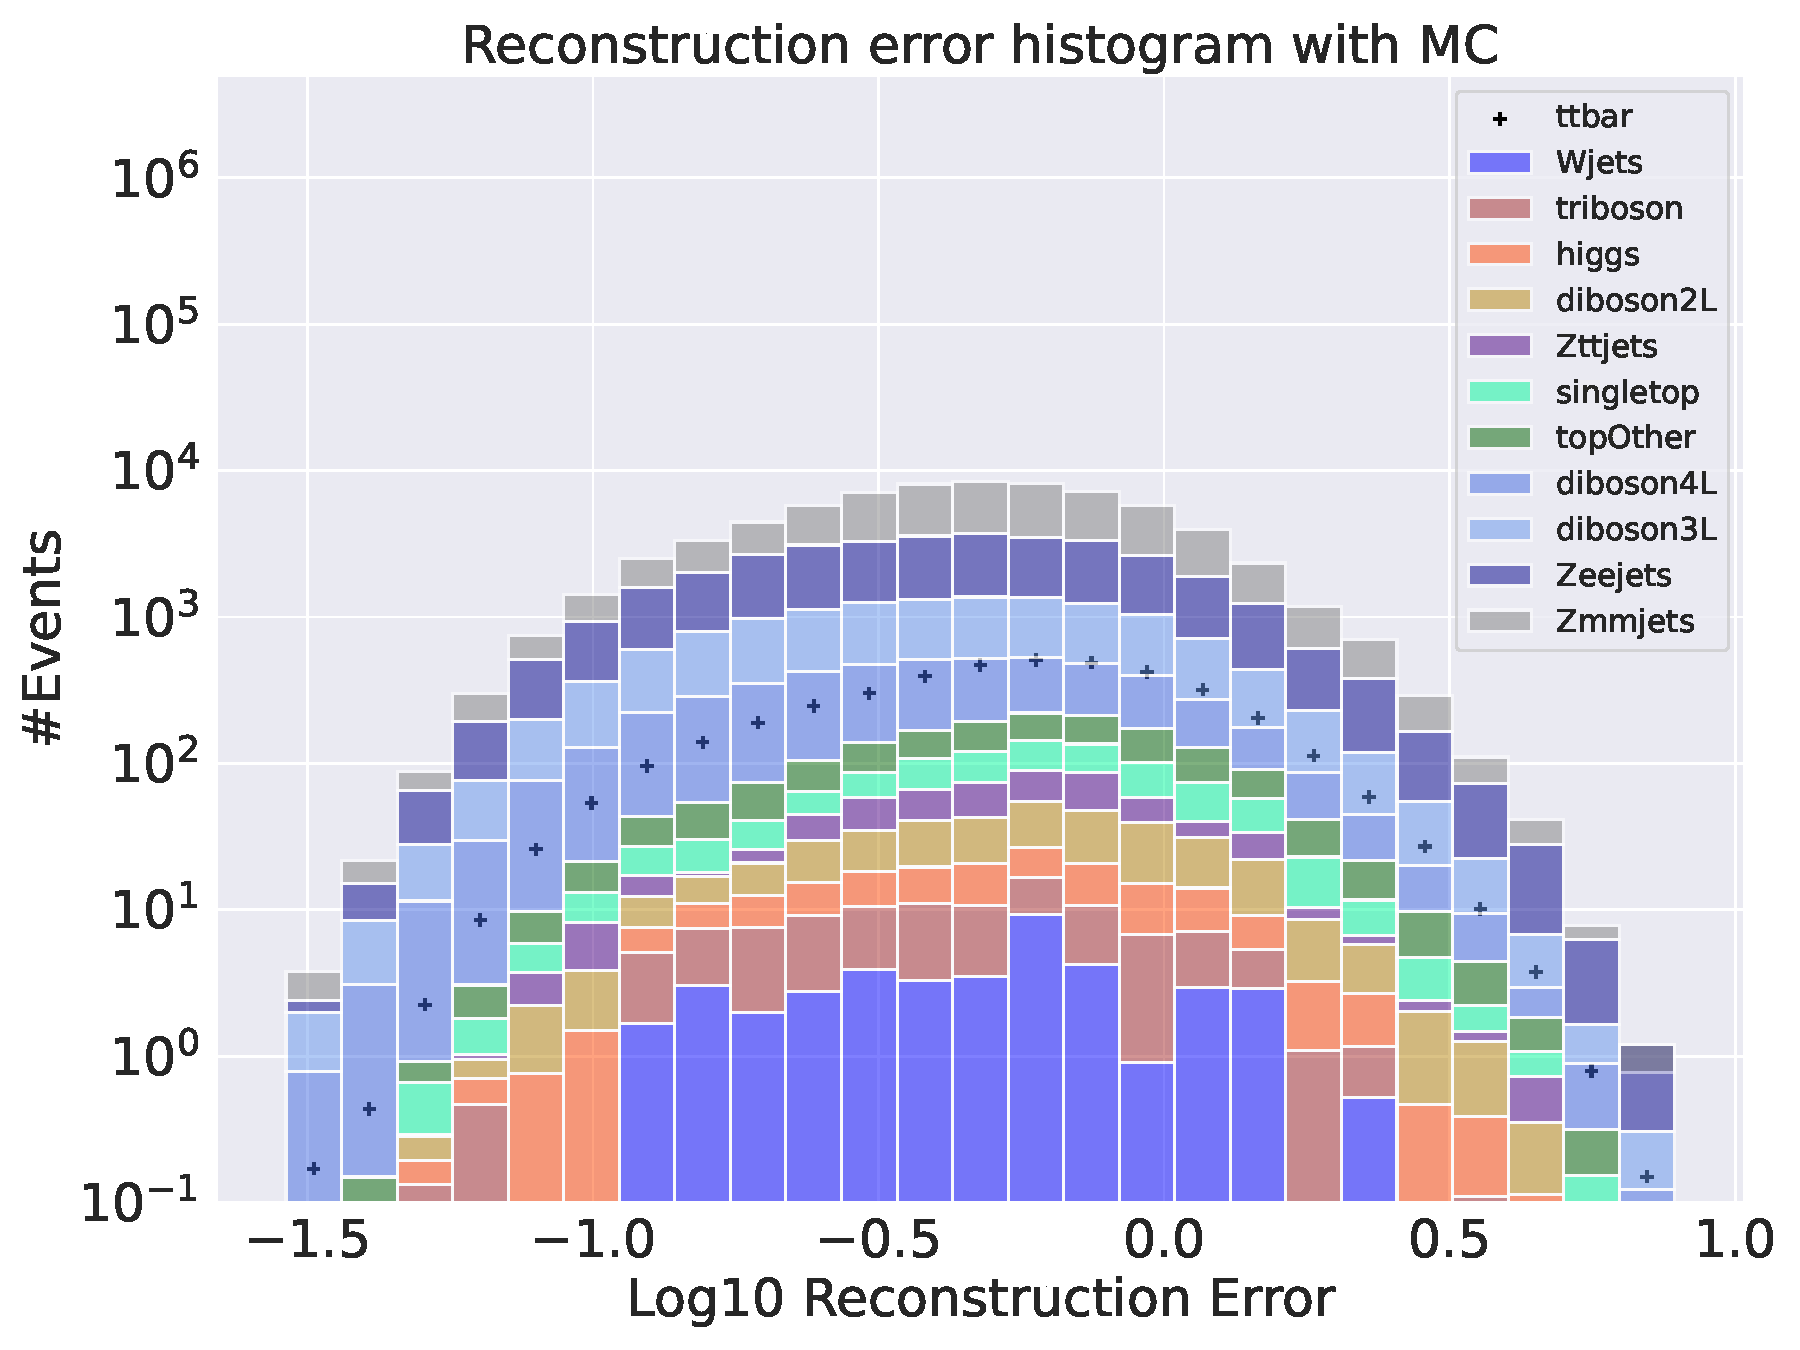
\includegraphics[width=\textwidth]{Figures/VAE_testing/big/b_data_recon_big_rm3_feats_sig_ttbar.pdf}
        \caption{Reconstruction error on validation SM MC from the big variational Autoencoder. Here the ttbar channel has been removed from training and 
        is used as signal. No significant difference in distributions are found. }
        \label{fig:vae_big_ttbar}
    \end{subfigure}
    \hfill 
    \label{fig:vae_big_channel_3}
\end{figure}

\newpage

\subsection*{Altering of transverse momentum}
Altering the transverse momentum of some particles would in the extreme be anomalous and the hypothesis was that some of those trends would be
picked up by the autoencoder. Several scales for the transverse momentum were used, with the following results.

\subsubsection*{Autoencoder}

\begin{figure}[h!]
    \centering
    \begin{subfigure}{.45\textwidth}
        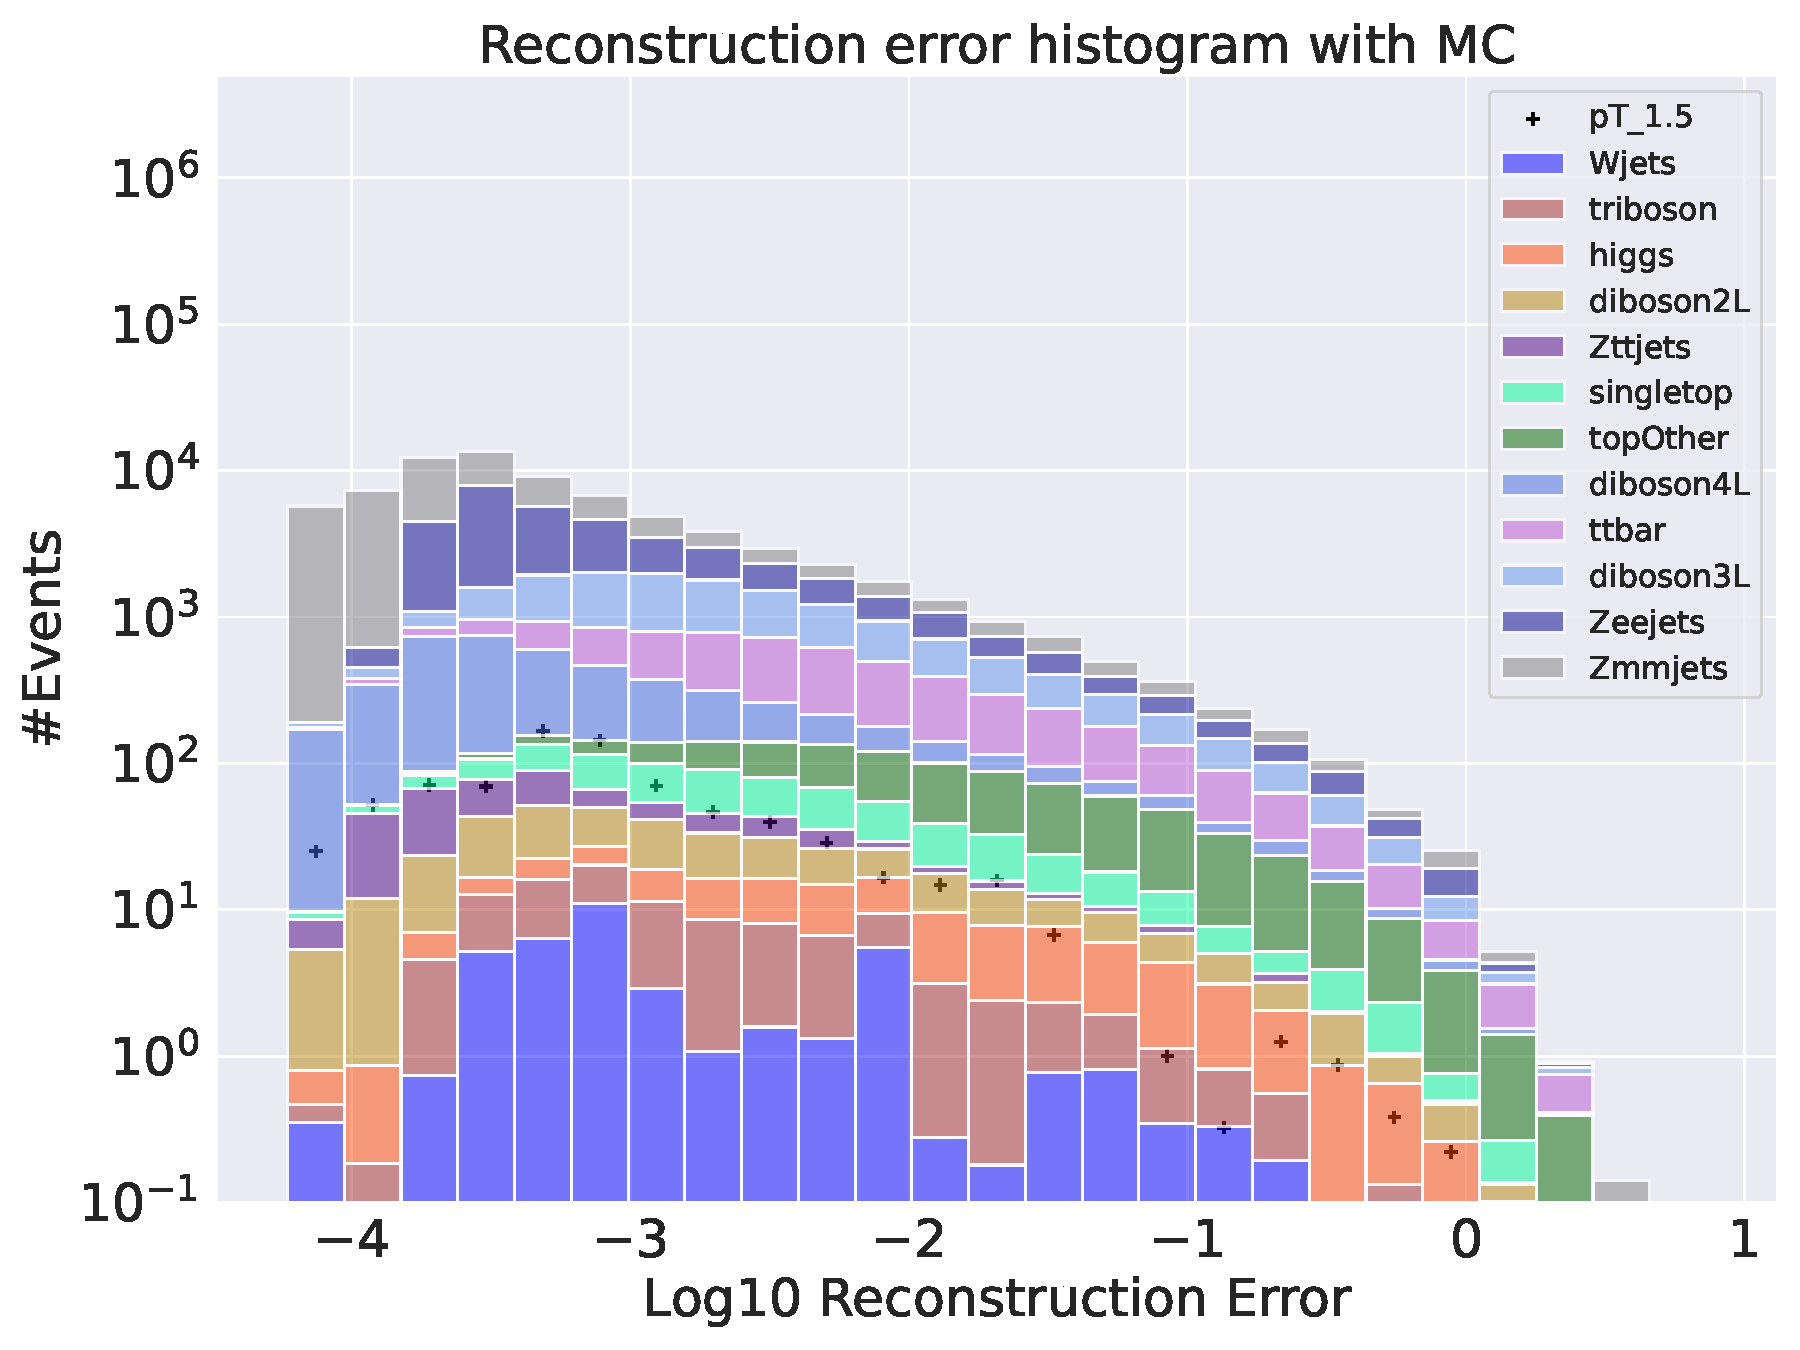
\includegraphics[width=\textwidth]{Figures/AE_testing/small/b_data_recon_big_rm3_feats_sig_pT_1.5.pdf}
        \caption{Reconstruction error on validation SM MC from the small variational Autoencoder. Here the signal is a subsample of the validation 
        set where the transverse momentum of the first electron and the first muon has been increased with a scale of $1.5$. The change of transverse 
        energy has thusly also been changed according to the scaling of transverse momentum. No significant difference in distributions are found. }
        \label{fig:ae_small_pt_1_5}
    \end{subfigure}
    \hfill 
    \begin{subfigure}{.45\textwidth}
        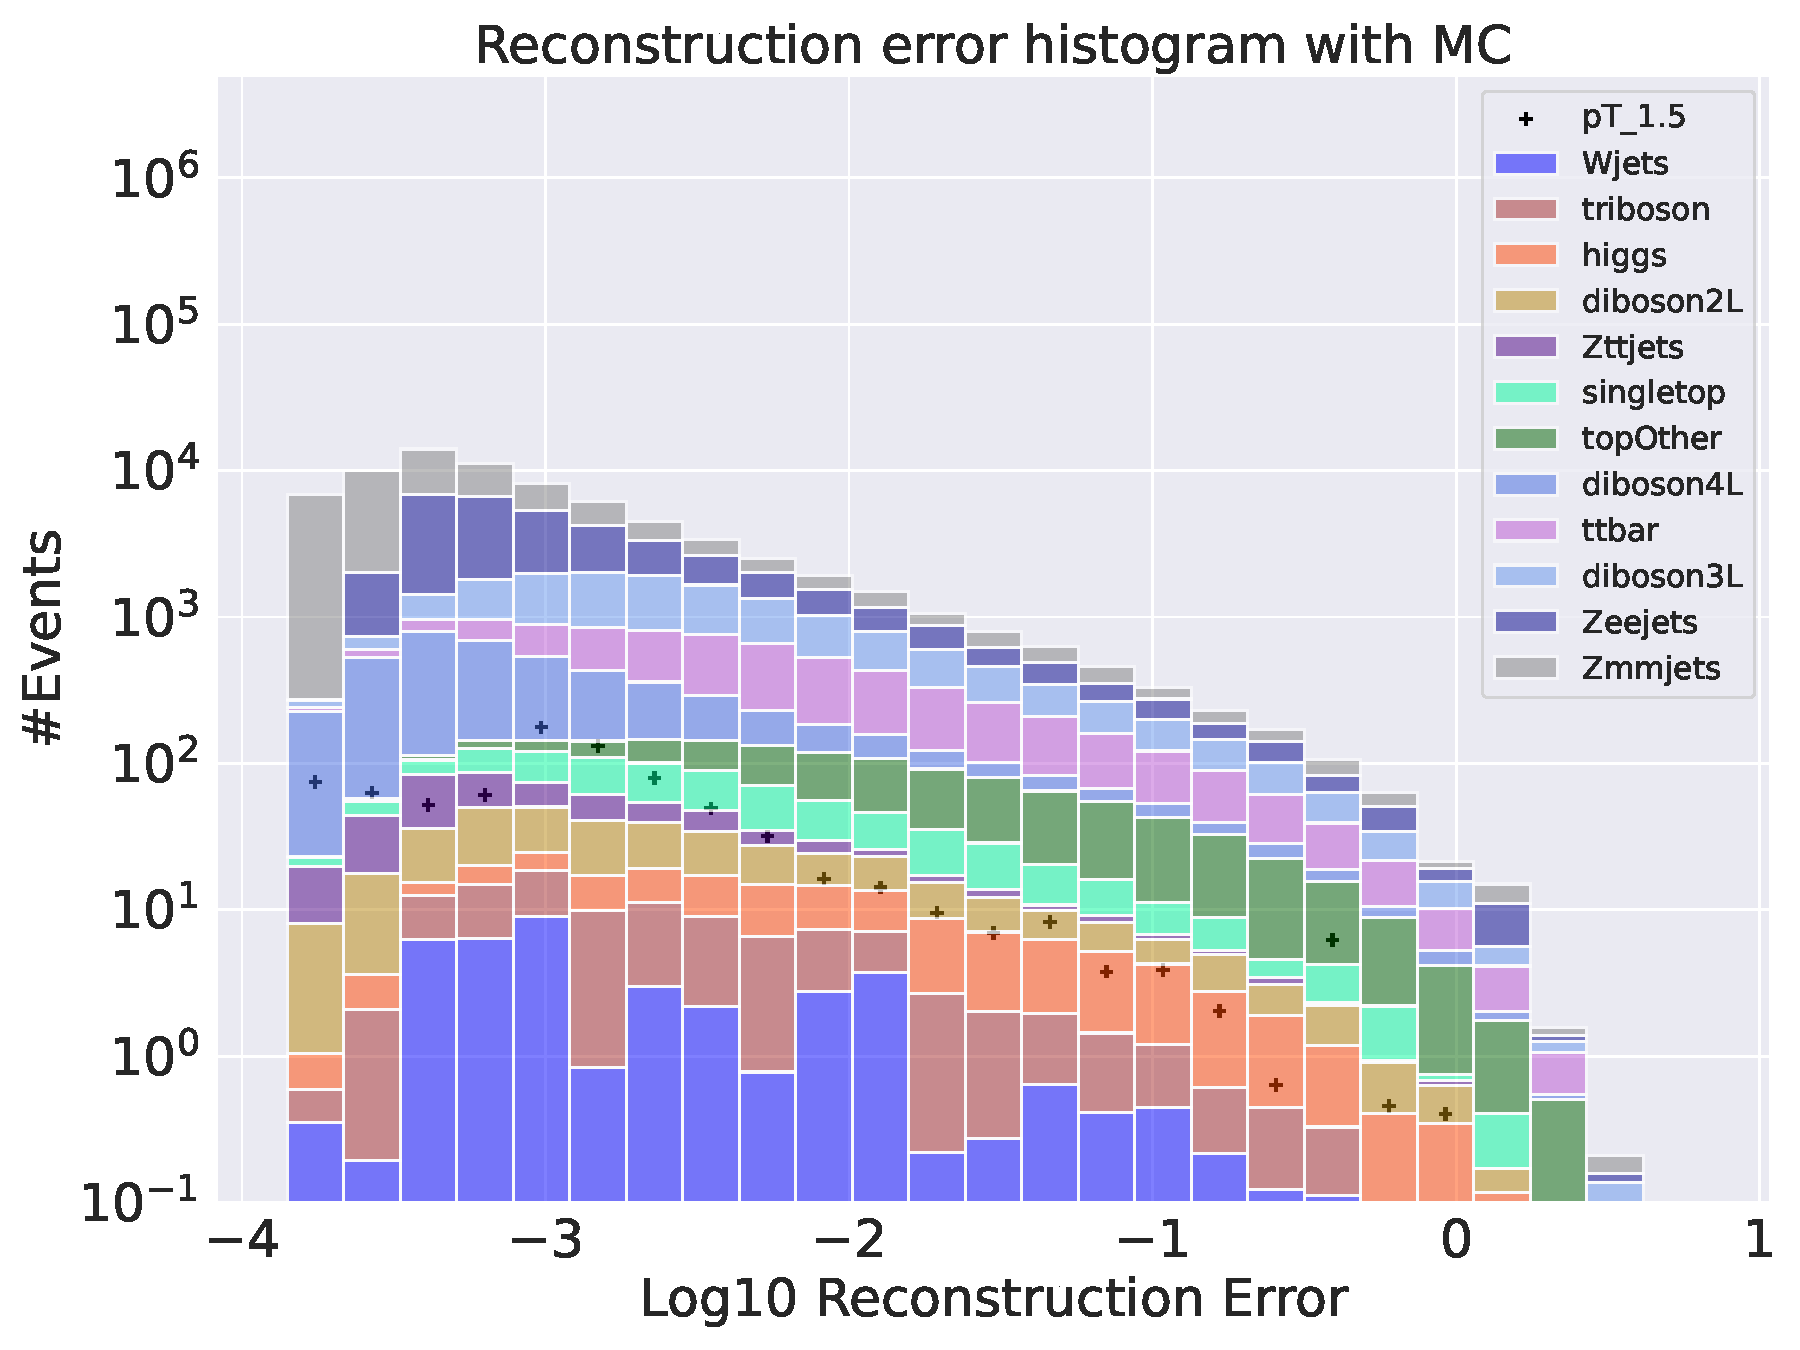
\includegraphics[width=\textwidth]{Figures/AE_testing/big/b_data_recon_big_rm3_feats_sig_pT_1.5.pdf}
        \caption{Reconstruction error on validation SM MC from the big variational Autoencoder.Here the signal is a subsample of the validation 
        set where the transverse momentum of the first electron and the first muon has been increased with a scale of $1.5$. The change of transverse 
        energy has thusly also been changed according to the scaling of transverse momentum. No significant difference in distributions are found. }
        \label{fig:ae_big_pt_1_5}
    \end{subfigure}
    \hfill 
    \label{fig:ae_big_small_pt_1_5}
\end{figure}

\begin{figure}[h!]
    \centering
    \begin{subfigure}{.45\textwidth}
        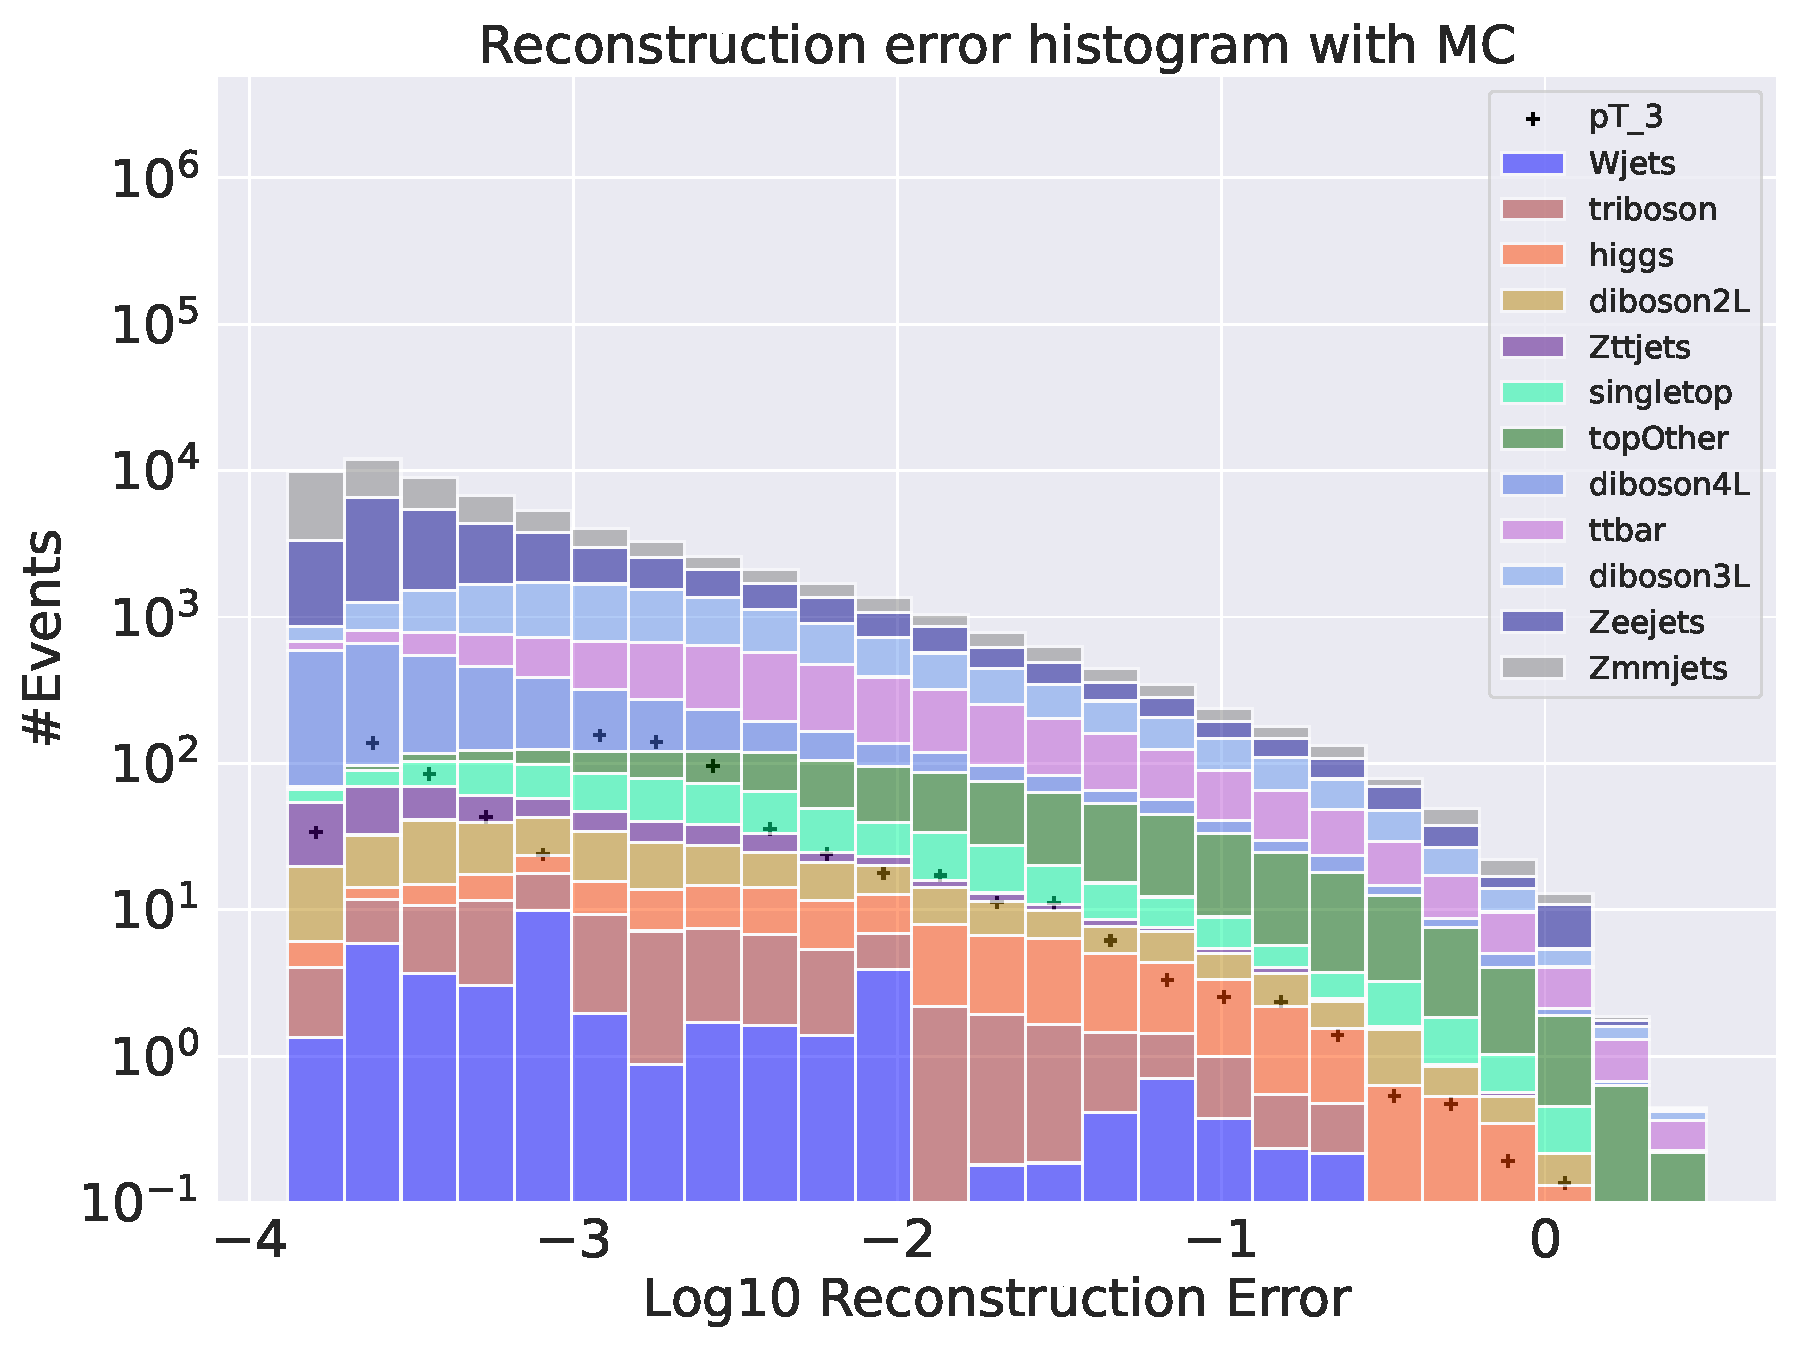
\includegraphics[width=\textwidth]{Figures/AE_testing/small/b_data_recon_big_rm3_feats_sig_pT_3.pdf}
        \caption{Reconstruction error on validation SM MC from the small variational Autoencoder. Here the signal is a subsample of the validation 
        set where the transverse momentum of the first electron and the first muon has been increased with a scale of $3$. The change of transverse 
        energy has thusly also been changed according to the scaling of transverse momentum. No significant difference in distributions are found. }
        \label{fig:ae_small_pt_3}
    \end{subfigure}
    \hfill 
    \begin{subfigure}{.45\textwidth}
        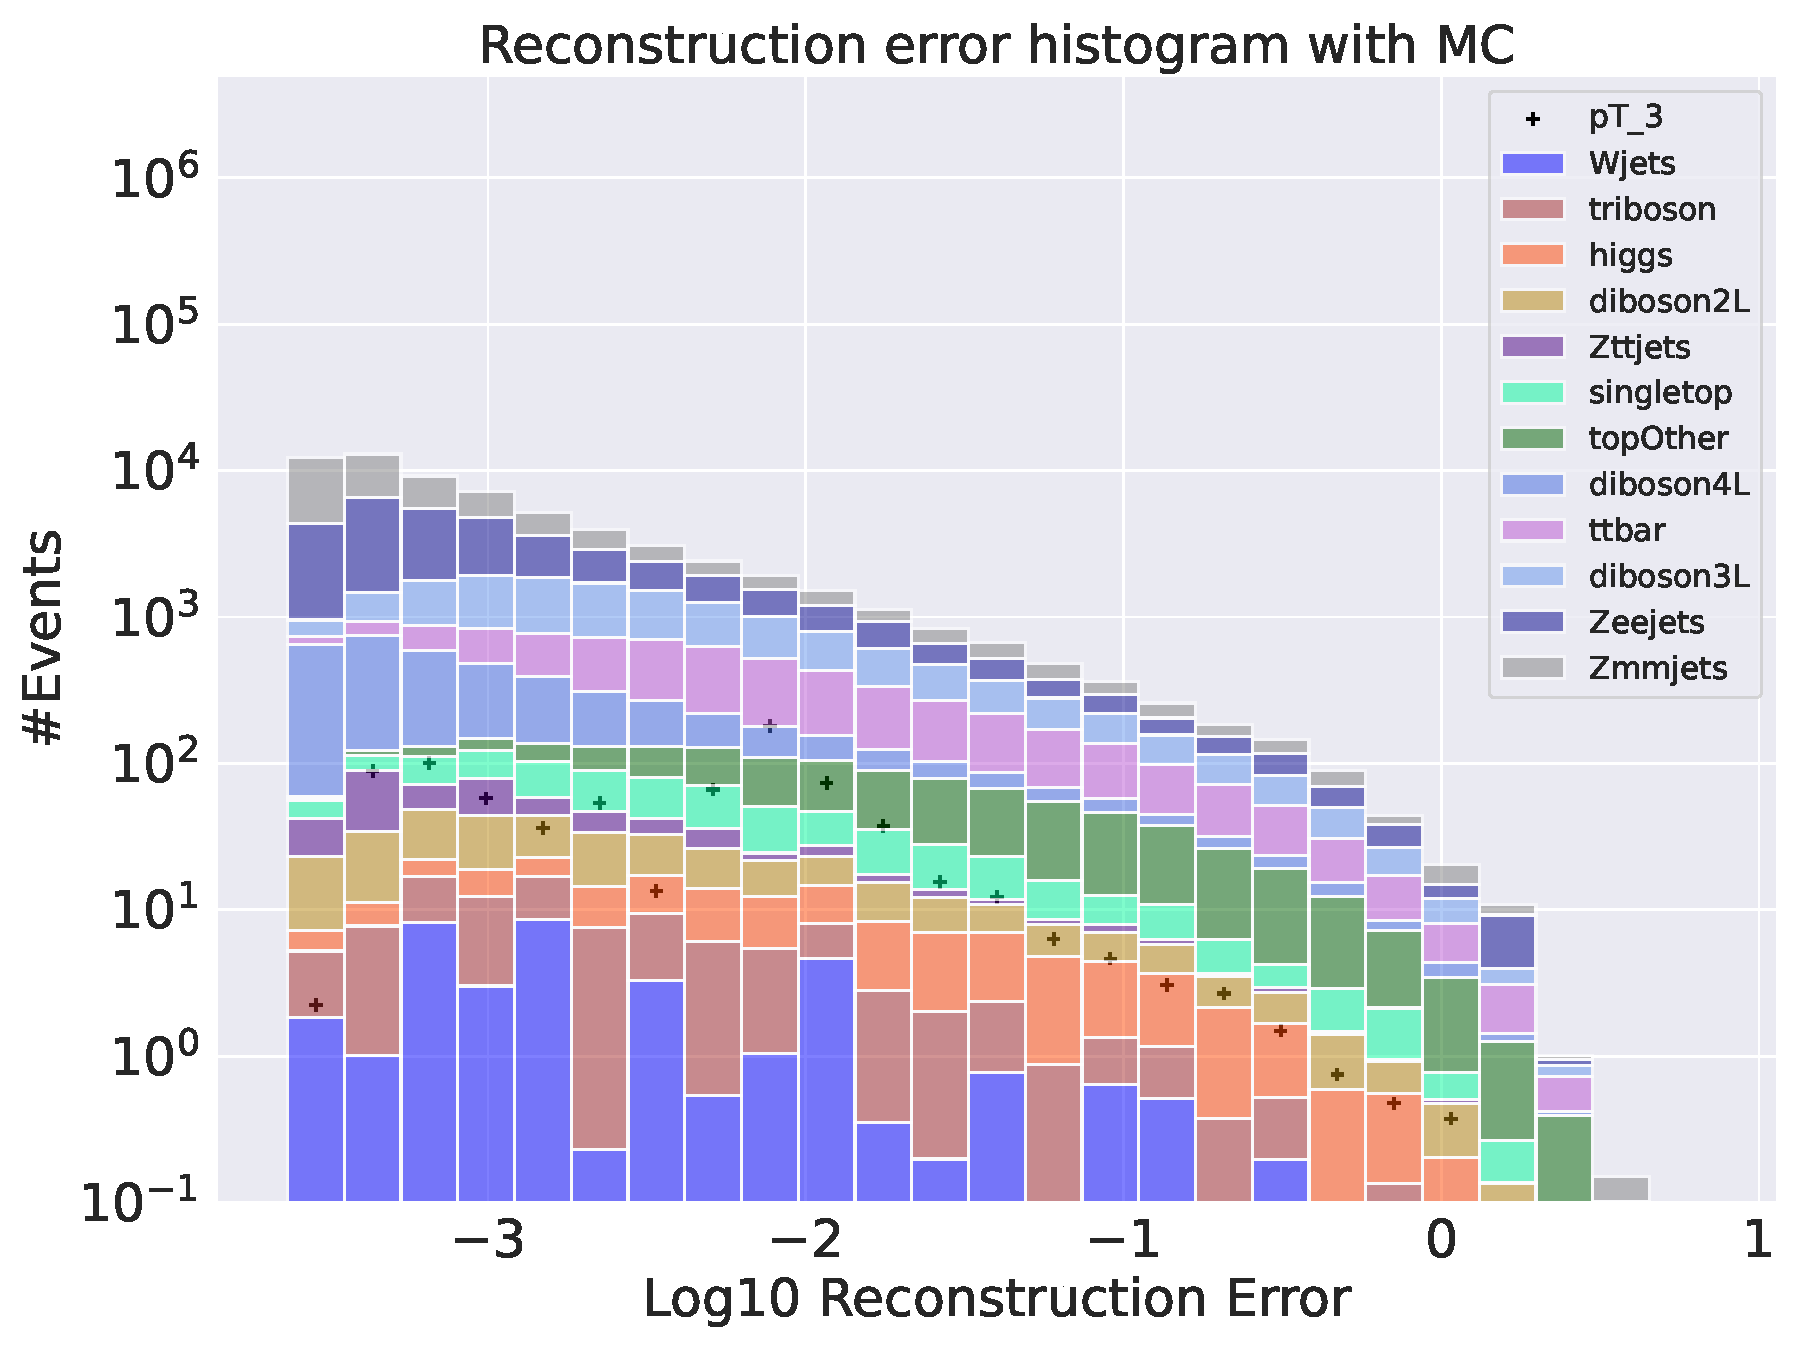
\includegraphics[width=\textwidth]{Figures/AE_testing/big/b_data_recon_big_rm3_feats_sig_pT_3.pdf}
        \caption{Reconstruction error on validation SM MC from the big variational Autoencoder. Here the signal is a subsample of the validation 
        set where the transverse momentum of the first electron and the first muon has been increased with a scale of $3$. The change of transverse 
        energy has thusly also been changed according to the scaling of transverse momentum. No significant difference in distributions are found. }
        \label{fig:ae_big_pt_3}
    \end{subfigure}
    \hfill 
    \label{fig:ae_big_small_pt_3}
\end{figure}

\begin{figure}[h!]
    \centering
    \begin{subfigure}{.45\textwidth}
        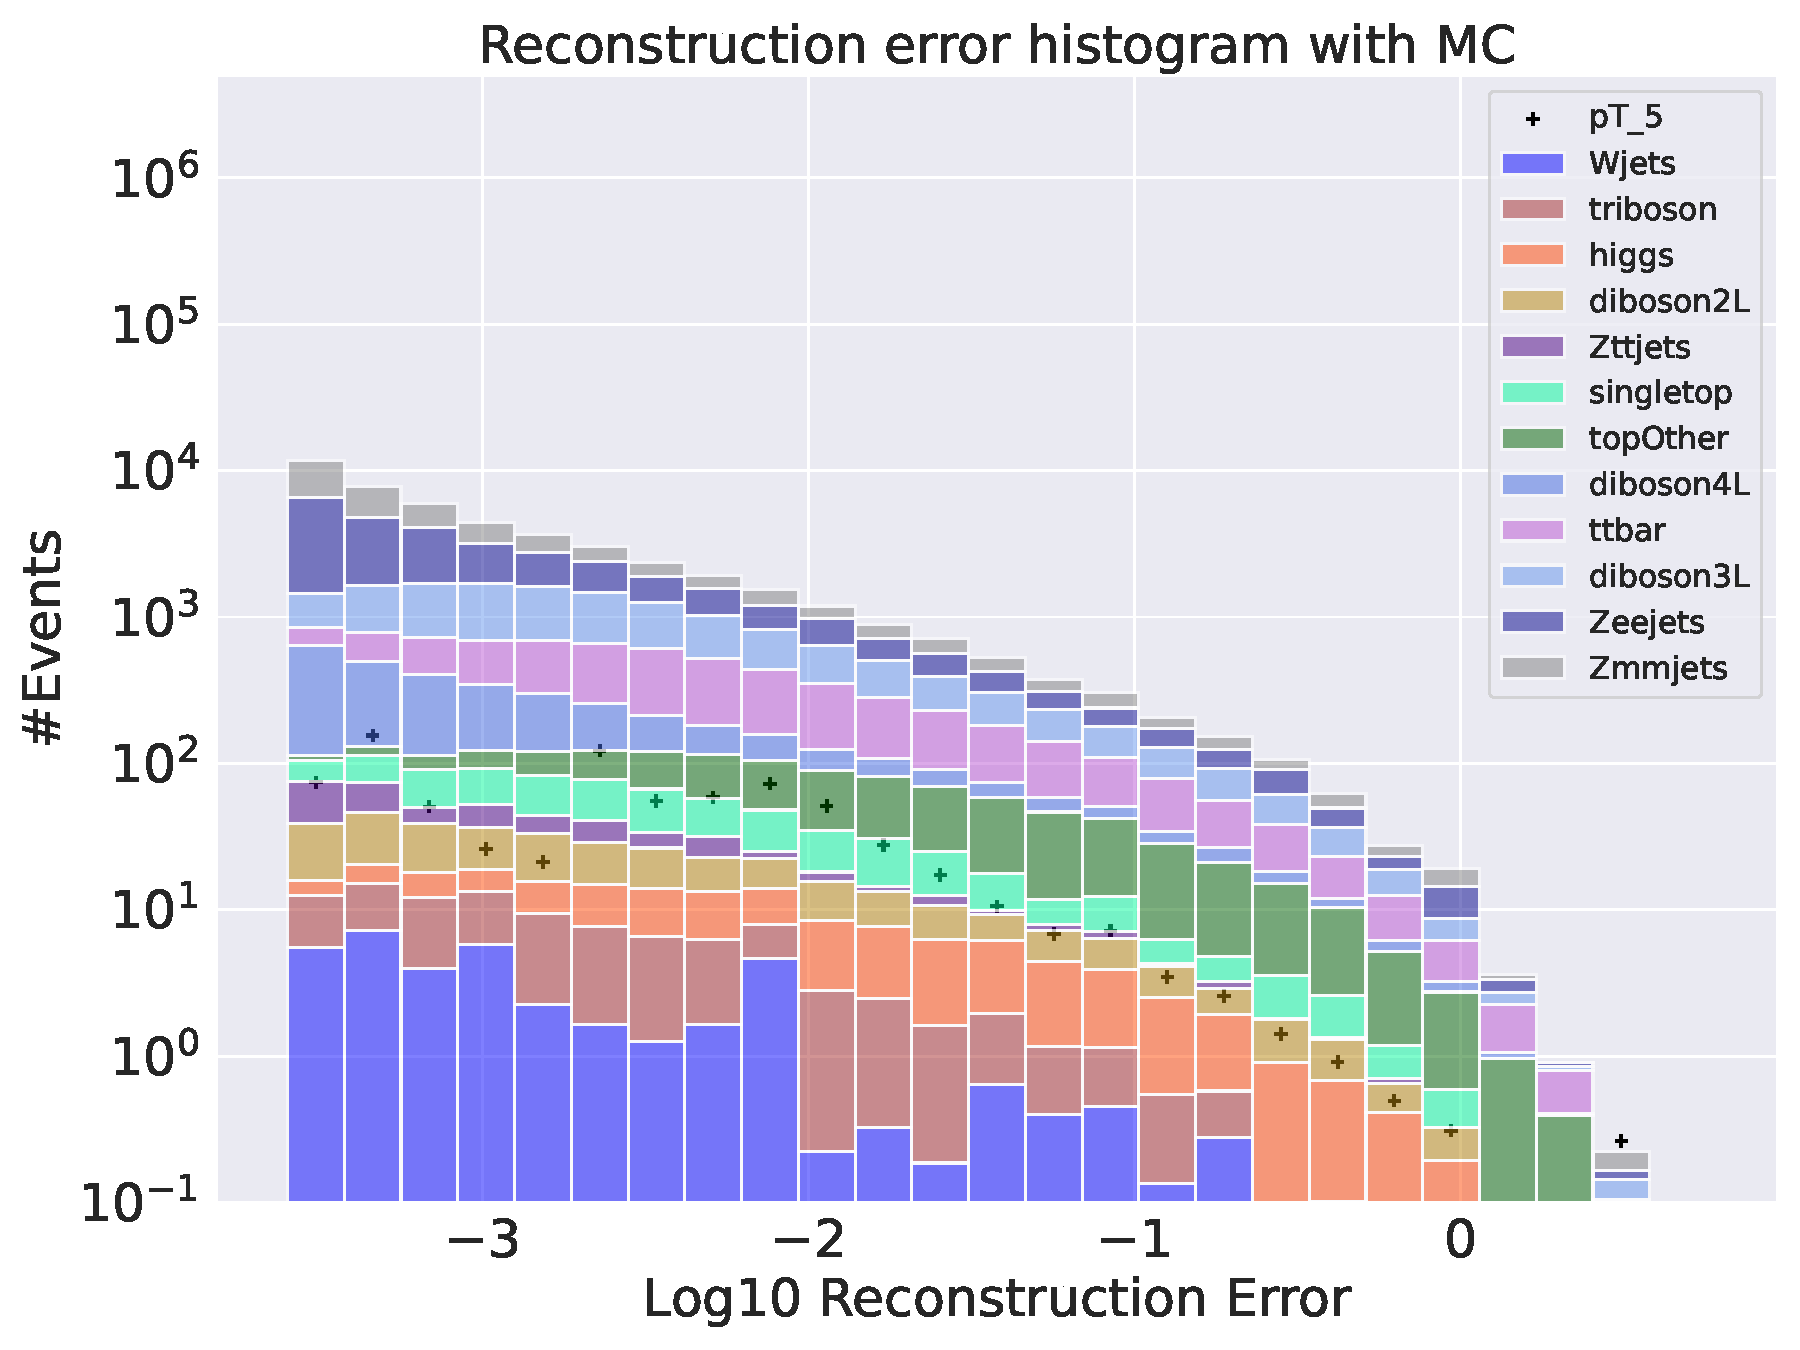
\includegraphics[width=\textwidth]{Figures/AE_testing/small/b_data_recon_big_rm3_feats_sig_pT_5.pdf}
        \caption{Reconstruction error on validation SM MC from the small variational Autoencoder. Here the signal is a subsample of the validation 
        set where the transverse momentum of the first electron and the first muon has been increased with a scale of $5$. The change of transverse 
        energy has thusly also been changed according to the scaling of transverse momentum. No significant difference in distributions are found. }
        \label{fig:ae_small_pt_5}
    \end{subfigure}
    \hfill 
    \begin{subfigure}{.45\textwidth}
        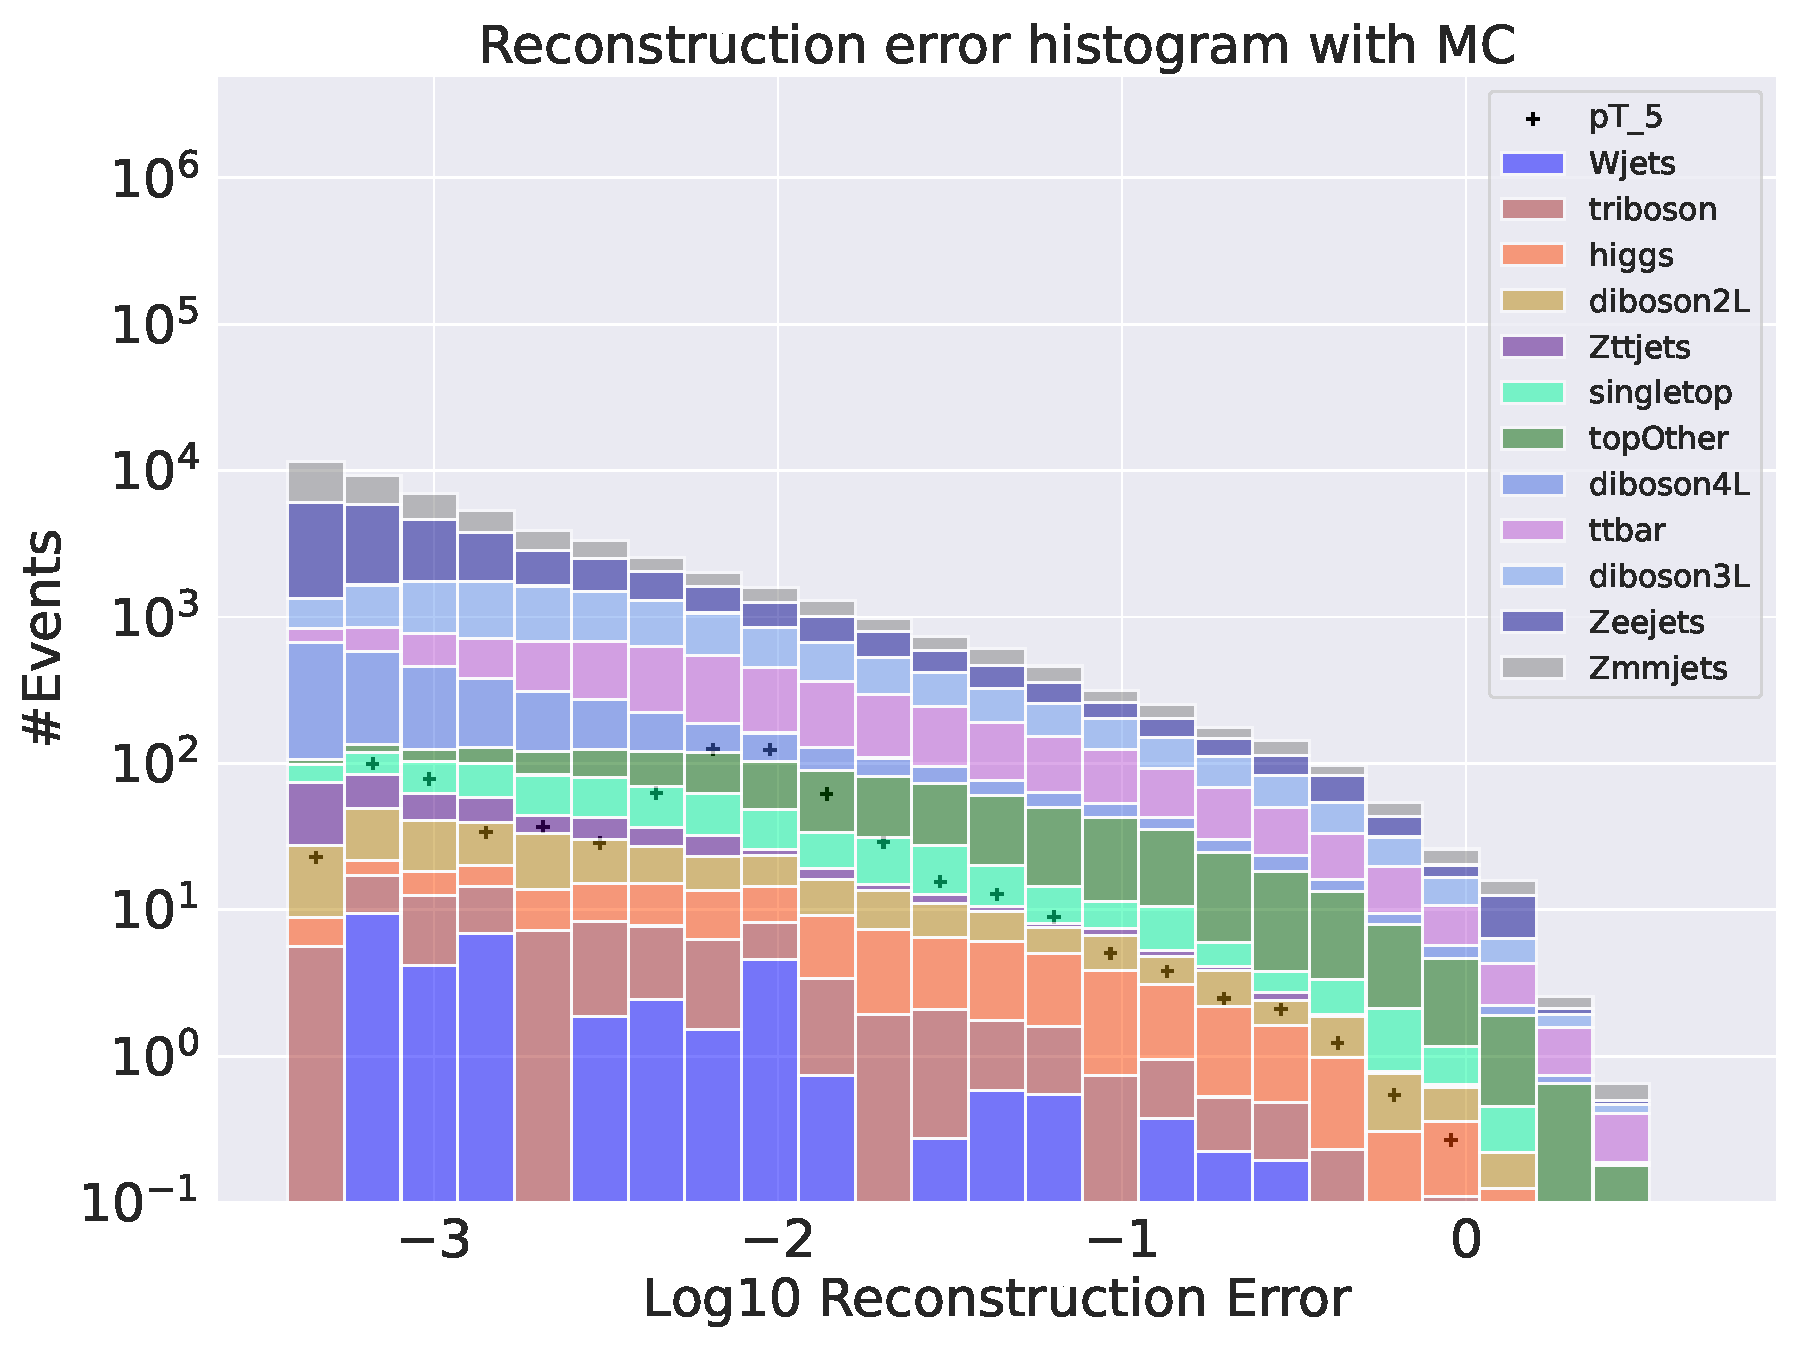
\includegraphics[width=\textwidth]{Figures/AE_testing/big/b_data_recon_big_rm3_feats_sig_pT_5.pdf}
        \caption{Reconstruction error on validation SM MC from the big variational Autoencoder. Here the signal is a subsample of the validation 
        set where the transverse momentum of the first electron and the first muon has been increased with a scale of $5$. The change of transverse 
        energy has thusly also been changed according to the scaling of transverse momentum. No significant difference in distributions are found. }
        \label{fig:ae_big_pt_5}
    \end{subfigure}
    \hfill 
    \label{fig:ae_big_small_pt_5}
\end{figure}


\begin{figure}[h!]
    \centering
    \begin{subfigure}{.45\textwidth}
        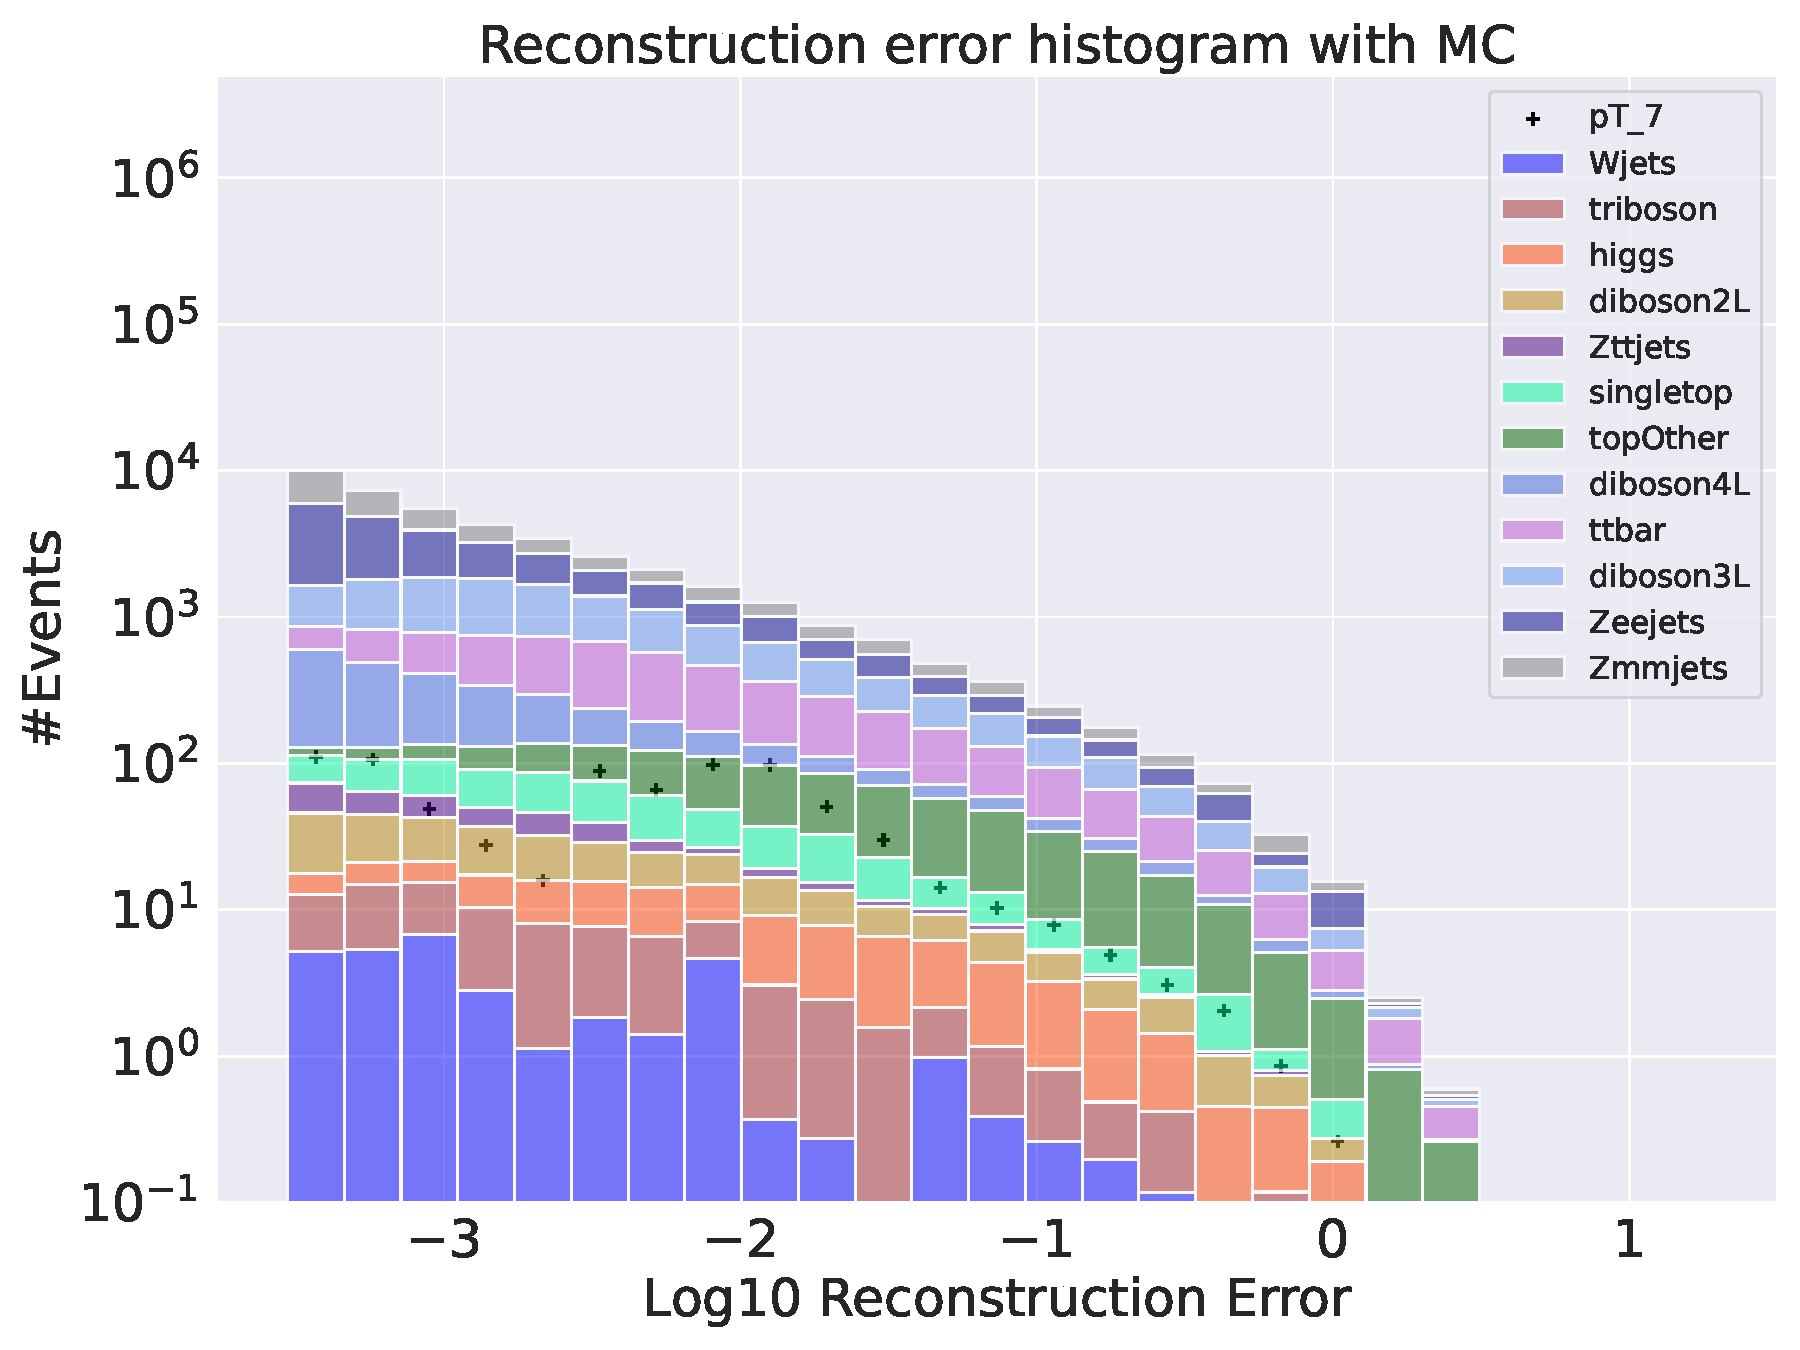
\includegraphics[width=\textwidth]{Figures/AE_testing/small/b_data_recon_big_rm3_feats_sig_pT_7.pdf}
        \caption{Reconstruction error on validation SM MC from the small variational Autoencoder. Here the signal is a subsample of the validation 
        set where the transverse momentum of the first electron and the first muon has been increased with a scale of $7$. The change of transverse 
        energy has thusly also been changed according to the scaling of transverse momentum. No significant difference in distributions are found. }
        \label{fig:ae_small_pt_7}
    \end{subfigure}
    \hfill 
    \begin{subfigure}{.45\textwidth}
        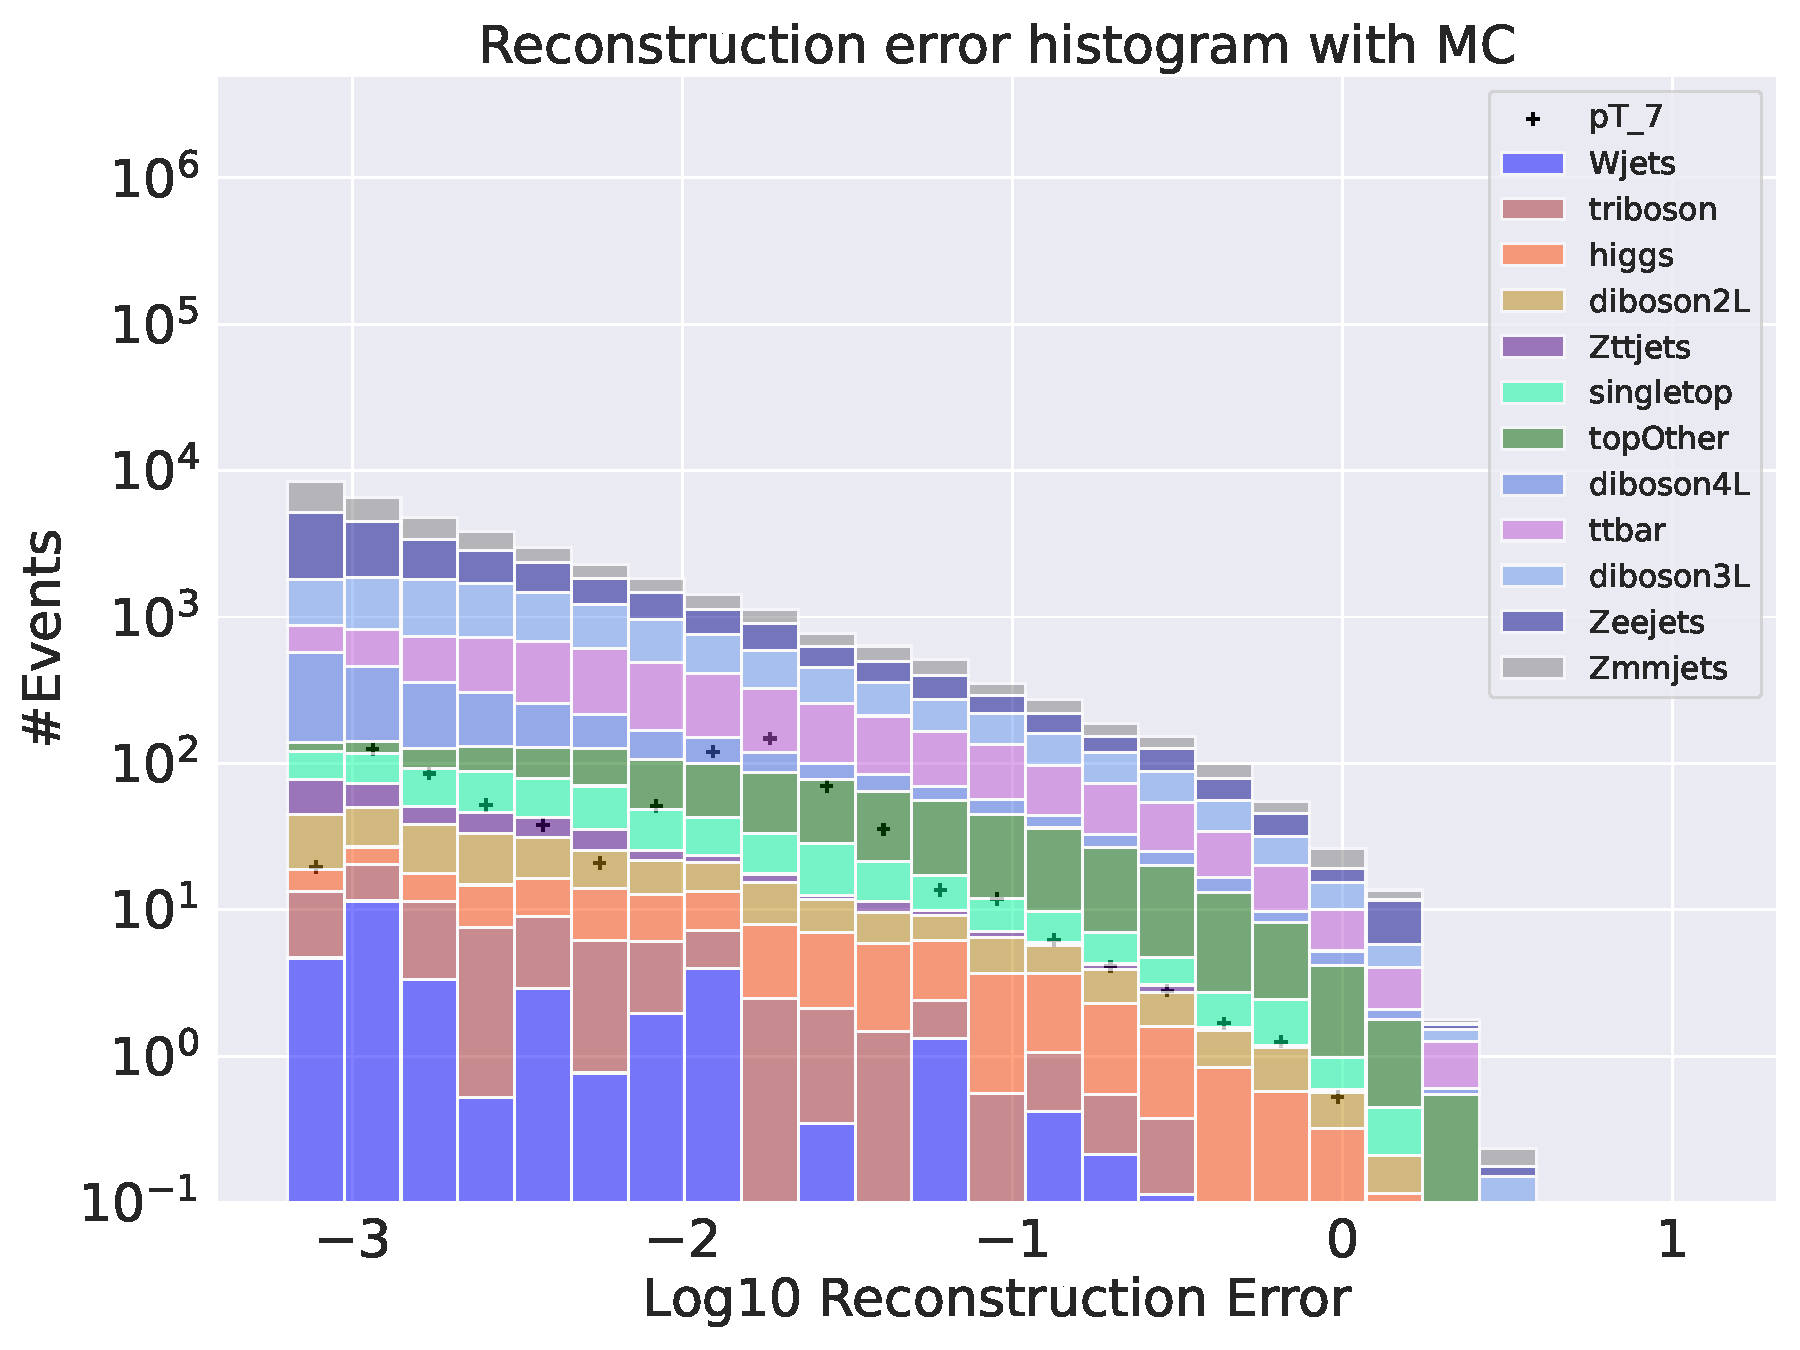
\includegraphics[width=\textwidth]{Figures/AE_testing/big/b_data_recon_big_rm3_feats_sig_pT_7.pdf}
        \caption{Reconstruction error on validation SM MC from the big variational Autoencoder. Here the signal is a subsample of the validation 
        set where the transverse momentum of the first electron and the first muon has been increased with a scale of $7$. The change of transverse 
        energy has thusly also been changed according to the scaling of transverse momentum. No significant difference in distributions are found. }
        \label{fig:ae_big_pt_7}
    \end{subfigure}
    \hfill 
    \label{fig:ae_big_small_pt_7}
\end{figure}

\begin{figure}[h!]
    \centering
    \begin{subfigure}{.45\textwidth}
        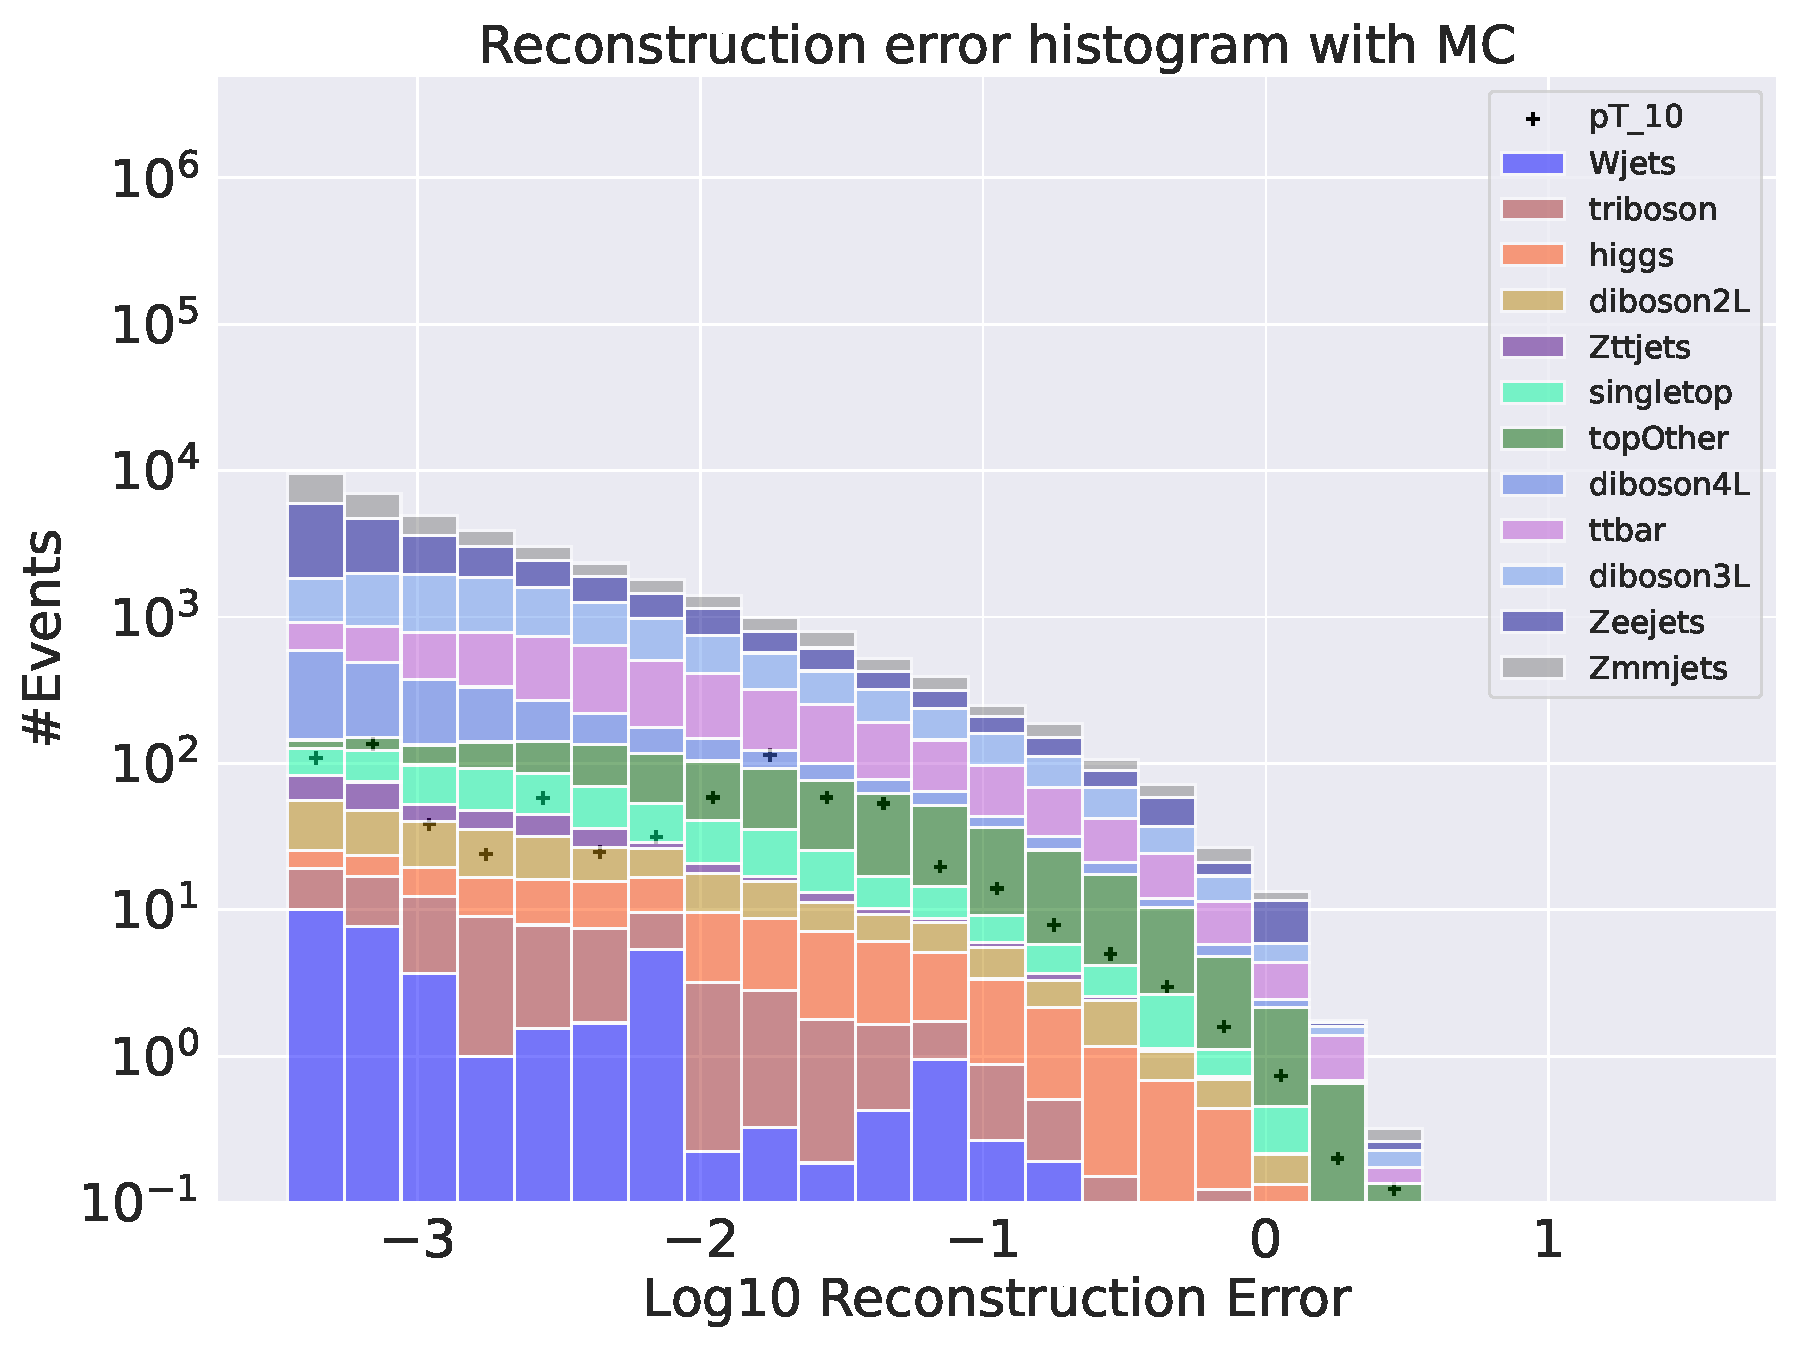
\includegraphics[width=\textwidth]{Figures/AE_testing/small/b_data_recon_big_rm3_feats_sig_pT_10.pdf}
        \caption{Reconstruction error on validation SM MC from the small variational Autoencoder. Here the signal is a subsample of the validation 
        set where the transverse momentum of the first electron and the first muon has been increased with a scale of $10$. The change of transverse 
        energy has thusly also been changed according to the scaling of transverse momentum. No significant difference in distributions are found. }
        \label{fig:ae_small_pt_10}
    \end{subfigure}
    \hfill 
    \begin{subfigure}{.45\textwidth}
        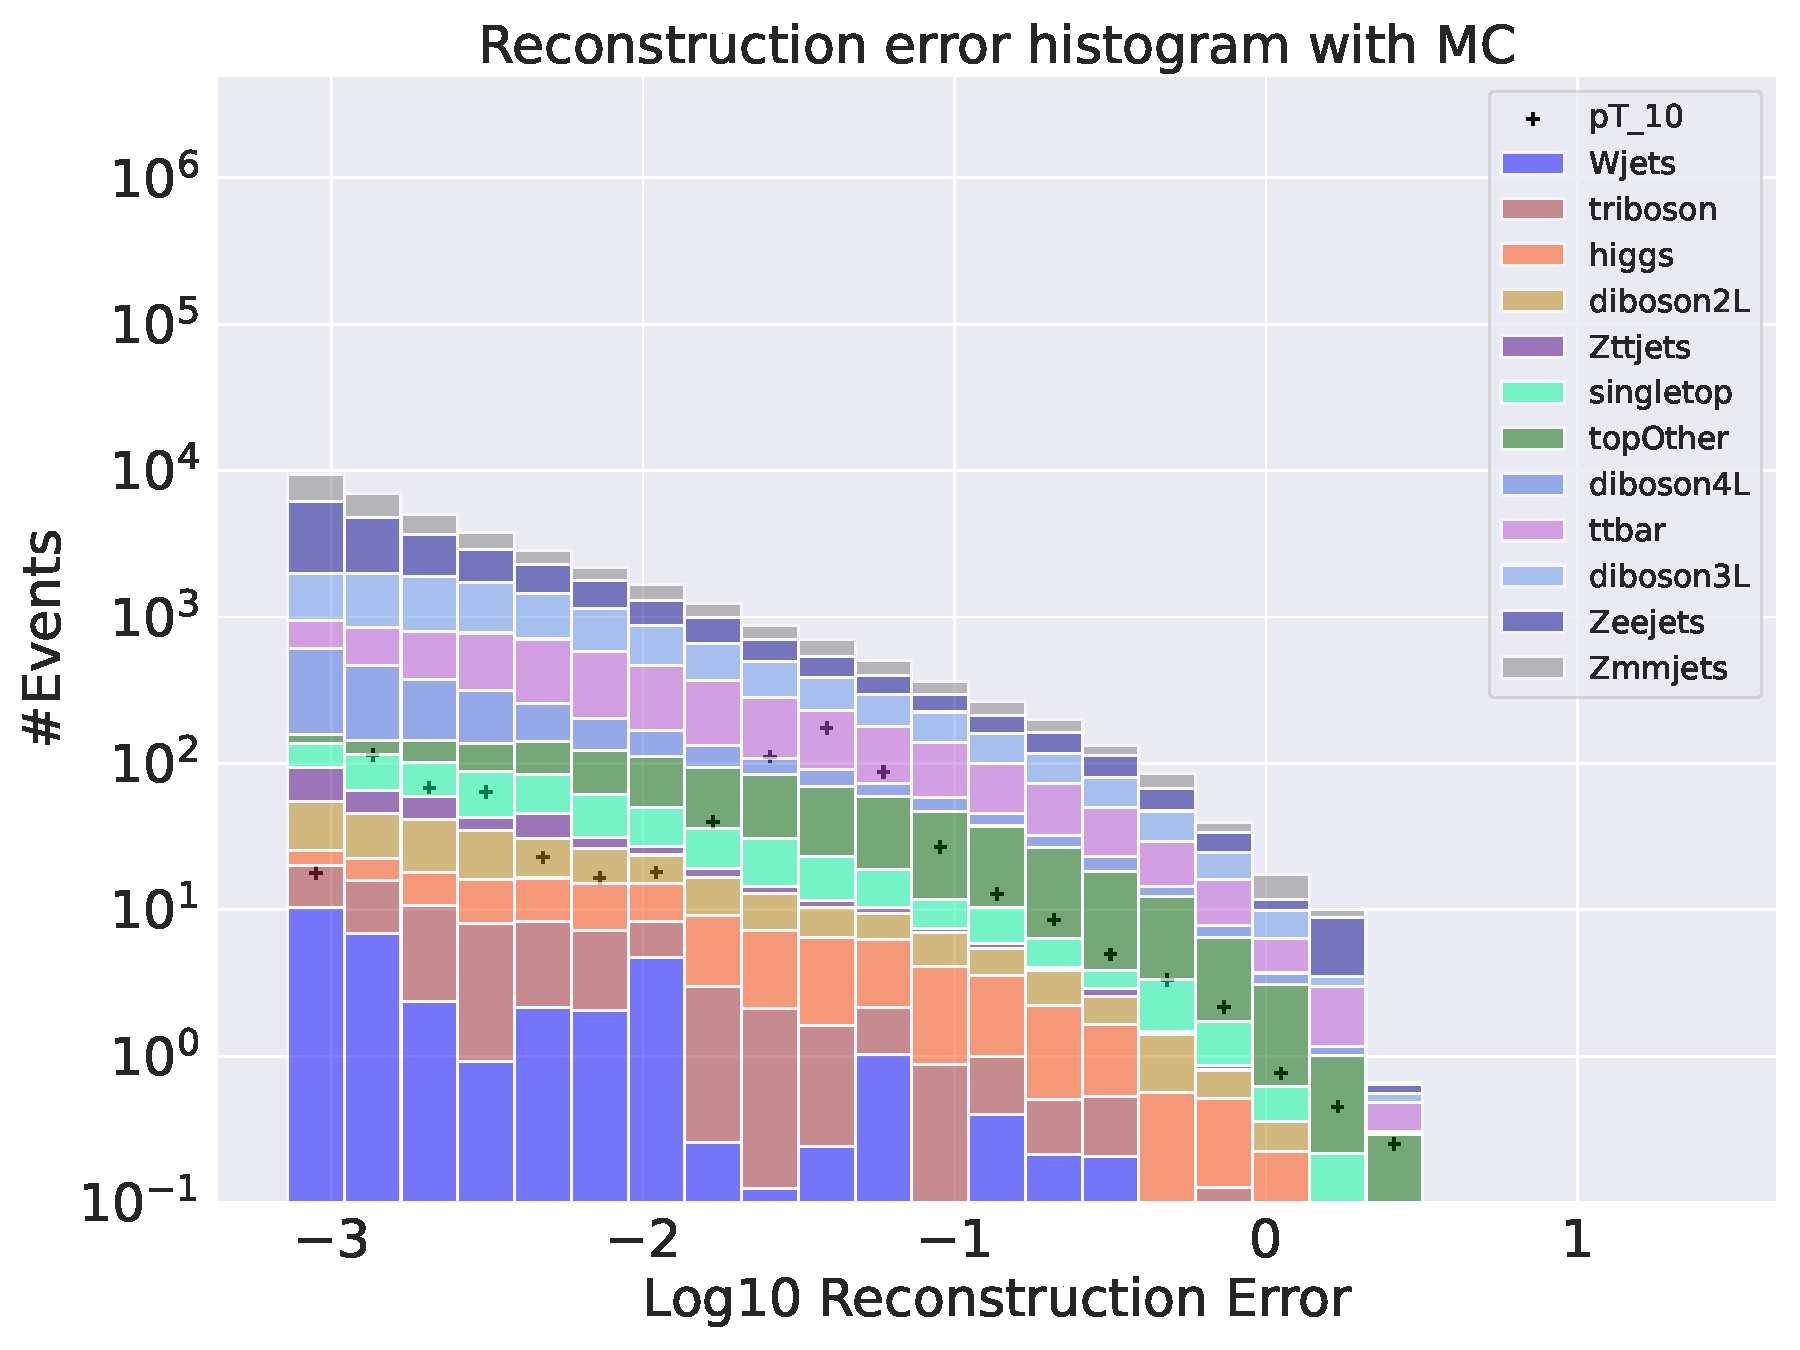
\includegraphics[width=\textwidth]{Figures/AE_testing/big/b_data_recon_big_rm3_feats_sig_pT_10.pdf}
        \caption{Reconstruction error on validation SM MC from the big variational Autoencoder. Here the signal is a subsample of the validation 
        set where the transverse momentum of the first electron and the first muon has been increased with a scale of $10$. The change of transverse 
        energy has thusly also been changed according to the scaling of transverse momentum. No significant difference in distributions are found. }
        \label{fig:ae_big_pt_10}
    \end{subfigure}
    \hfill 
    \label{fig:ae_big_small_pt_10}
\end{figure}



\subsubsection*{Variational Autoencoder}

\begin{figure}[h!]
    \centering
    \begin{subfigure}{.45\textwidth}
        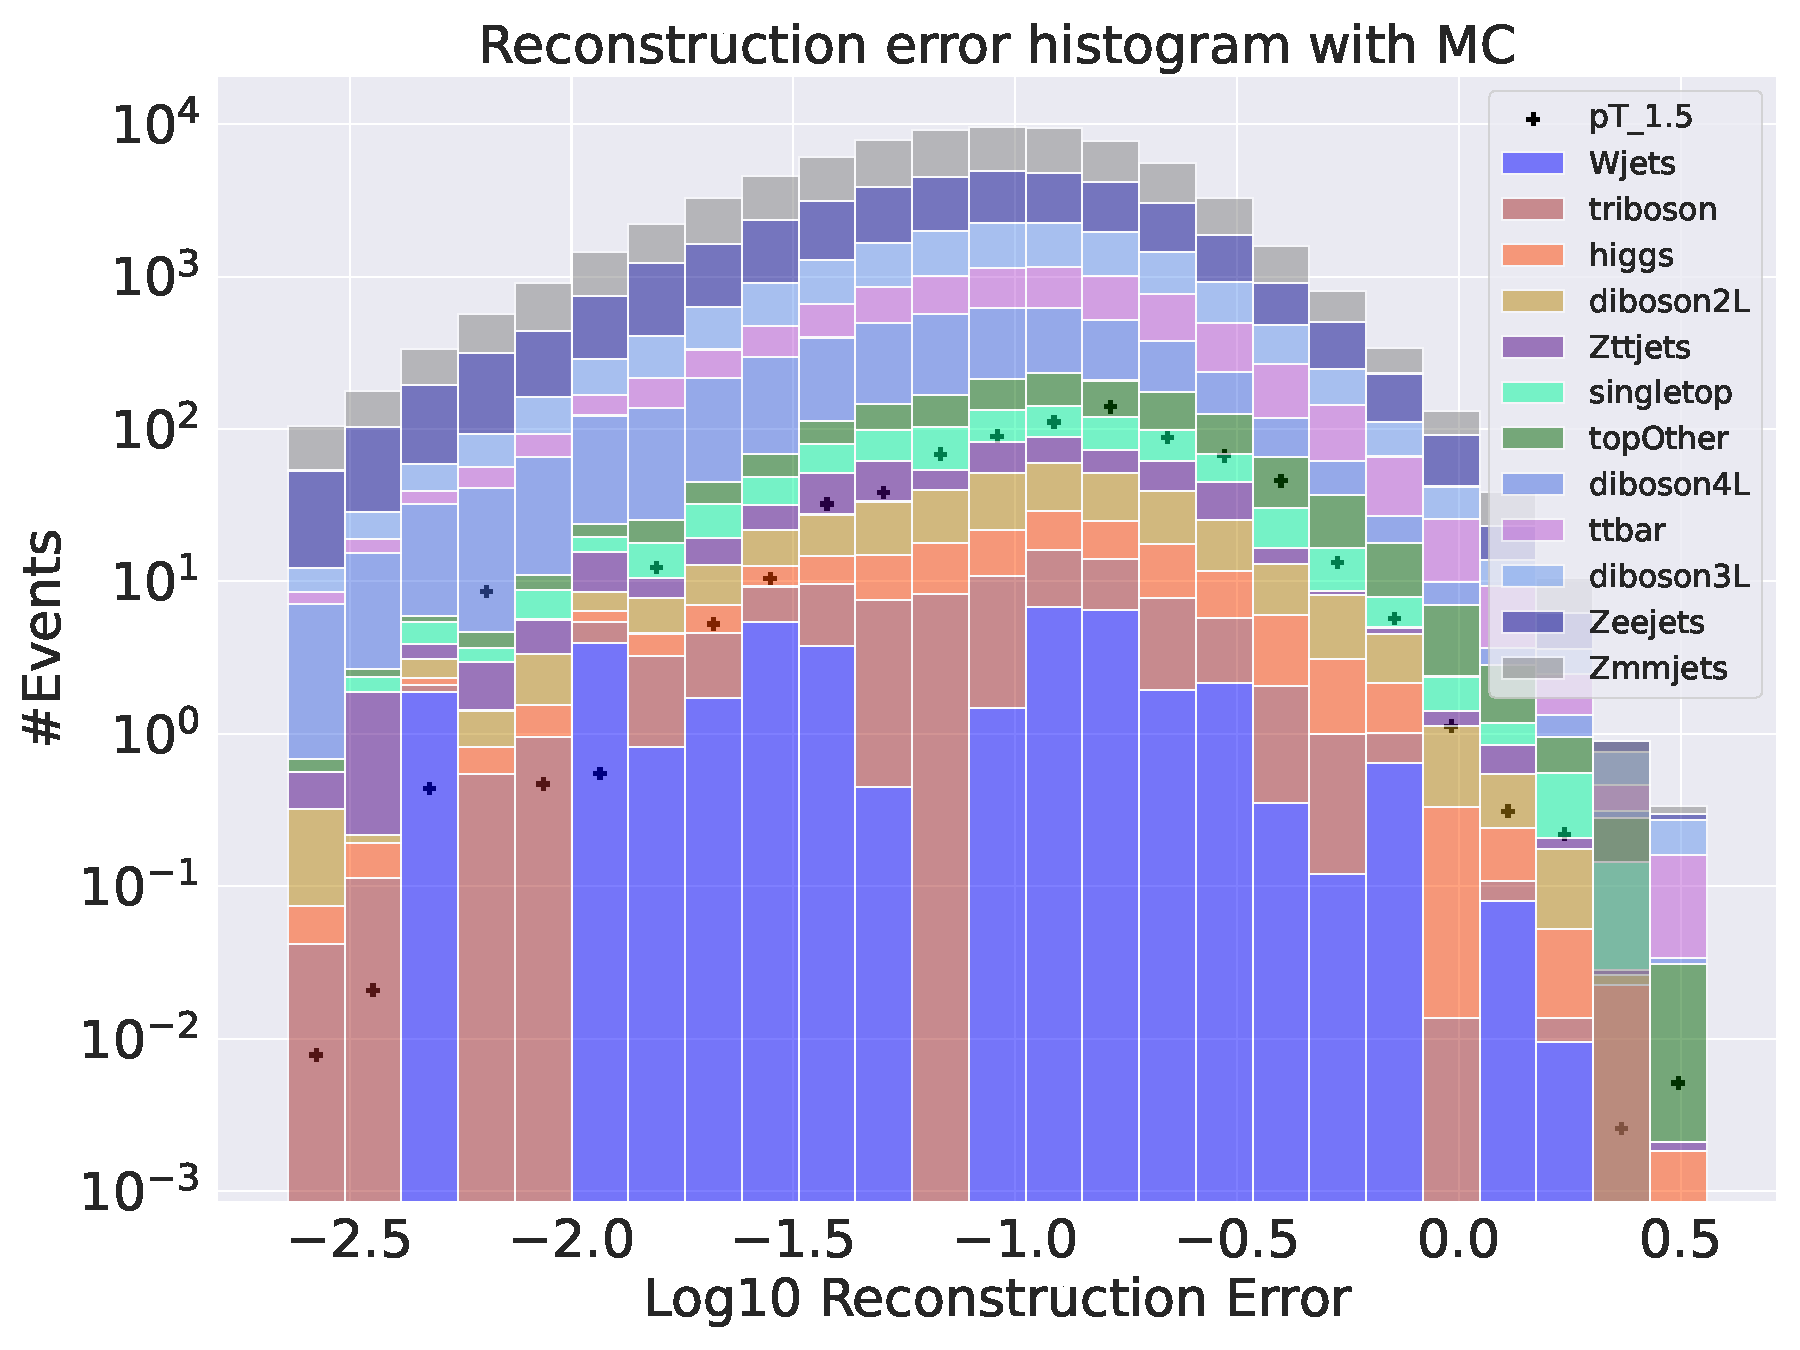
\includegraphics[width=\textwidth]{Figures/VAE_testing/small/b_data_recon_big_rm3_feats_sig_pT_1.5.pdf}
        \caption{Reconstruction error on validation SM MC from the small variational Autoencoder. Here the signal is a subsample of the validation 
        set where the transverse momentum of the first electron and the first muon has been increased with a scale of $1.5$. The change of transverse 
        energy has thusly also been changed according to the scaling of transverse momentum. No significant difference in distributions are found. }
        \label{fig:VAE_small_pt_1_5}
    \end{subfigure}
    \hfill 
    \begin{subfigure}{.45\textwidth}
        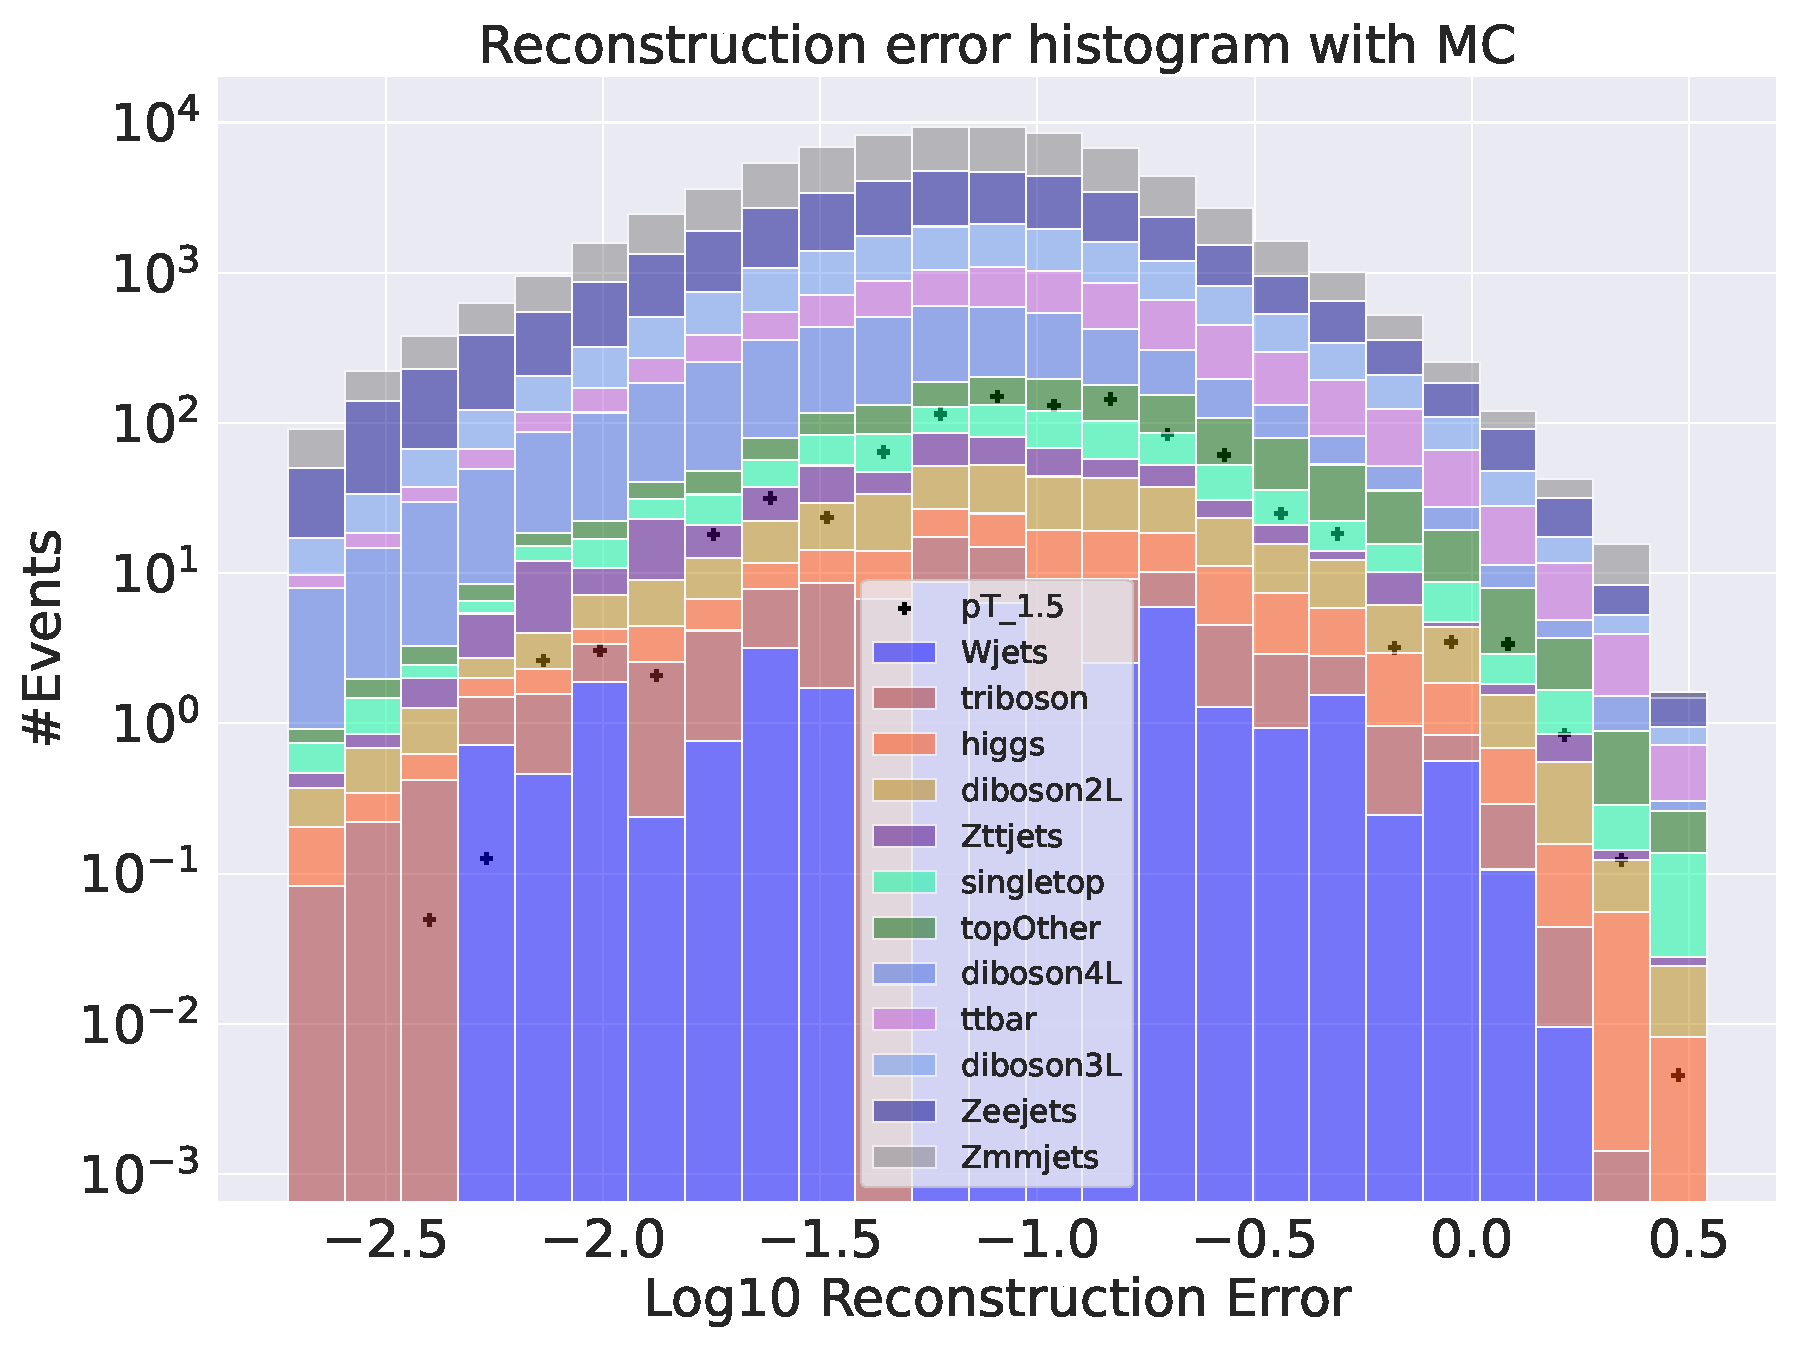
\includegraphics[width=\textwidth]{Figures/VAE_testing/big/b_data_recon_big_rm3_feats_sig_pT_1.5.pdf}
        \caption{Reconstruction error on validation SM MC from the big variational Autoencoder. Here the signal is a subsample of the validation 
        set where the transverse momentum of the first electron and the first muon has been increased with a scale of $1.5$. The change of transverse 
        energy has thusly also been changed according to the scaling of transverse momentum. No significant difference in distributions are found. }
        \label{fig:VAE_big_pt_1_5}
    \end{subfigure}
    \hfill 
    \label{fig:VAE_big_small_pt_1_5}
\end{figure}

\begin{figure}[h!]
    \centering
    \begin{subfigure}{.45\textwidth}
        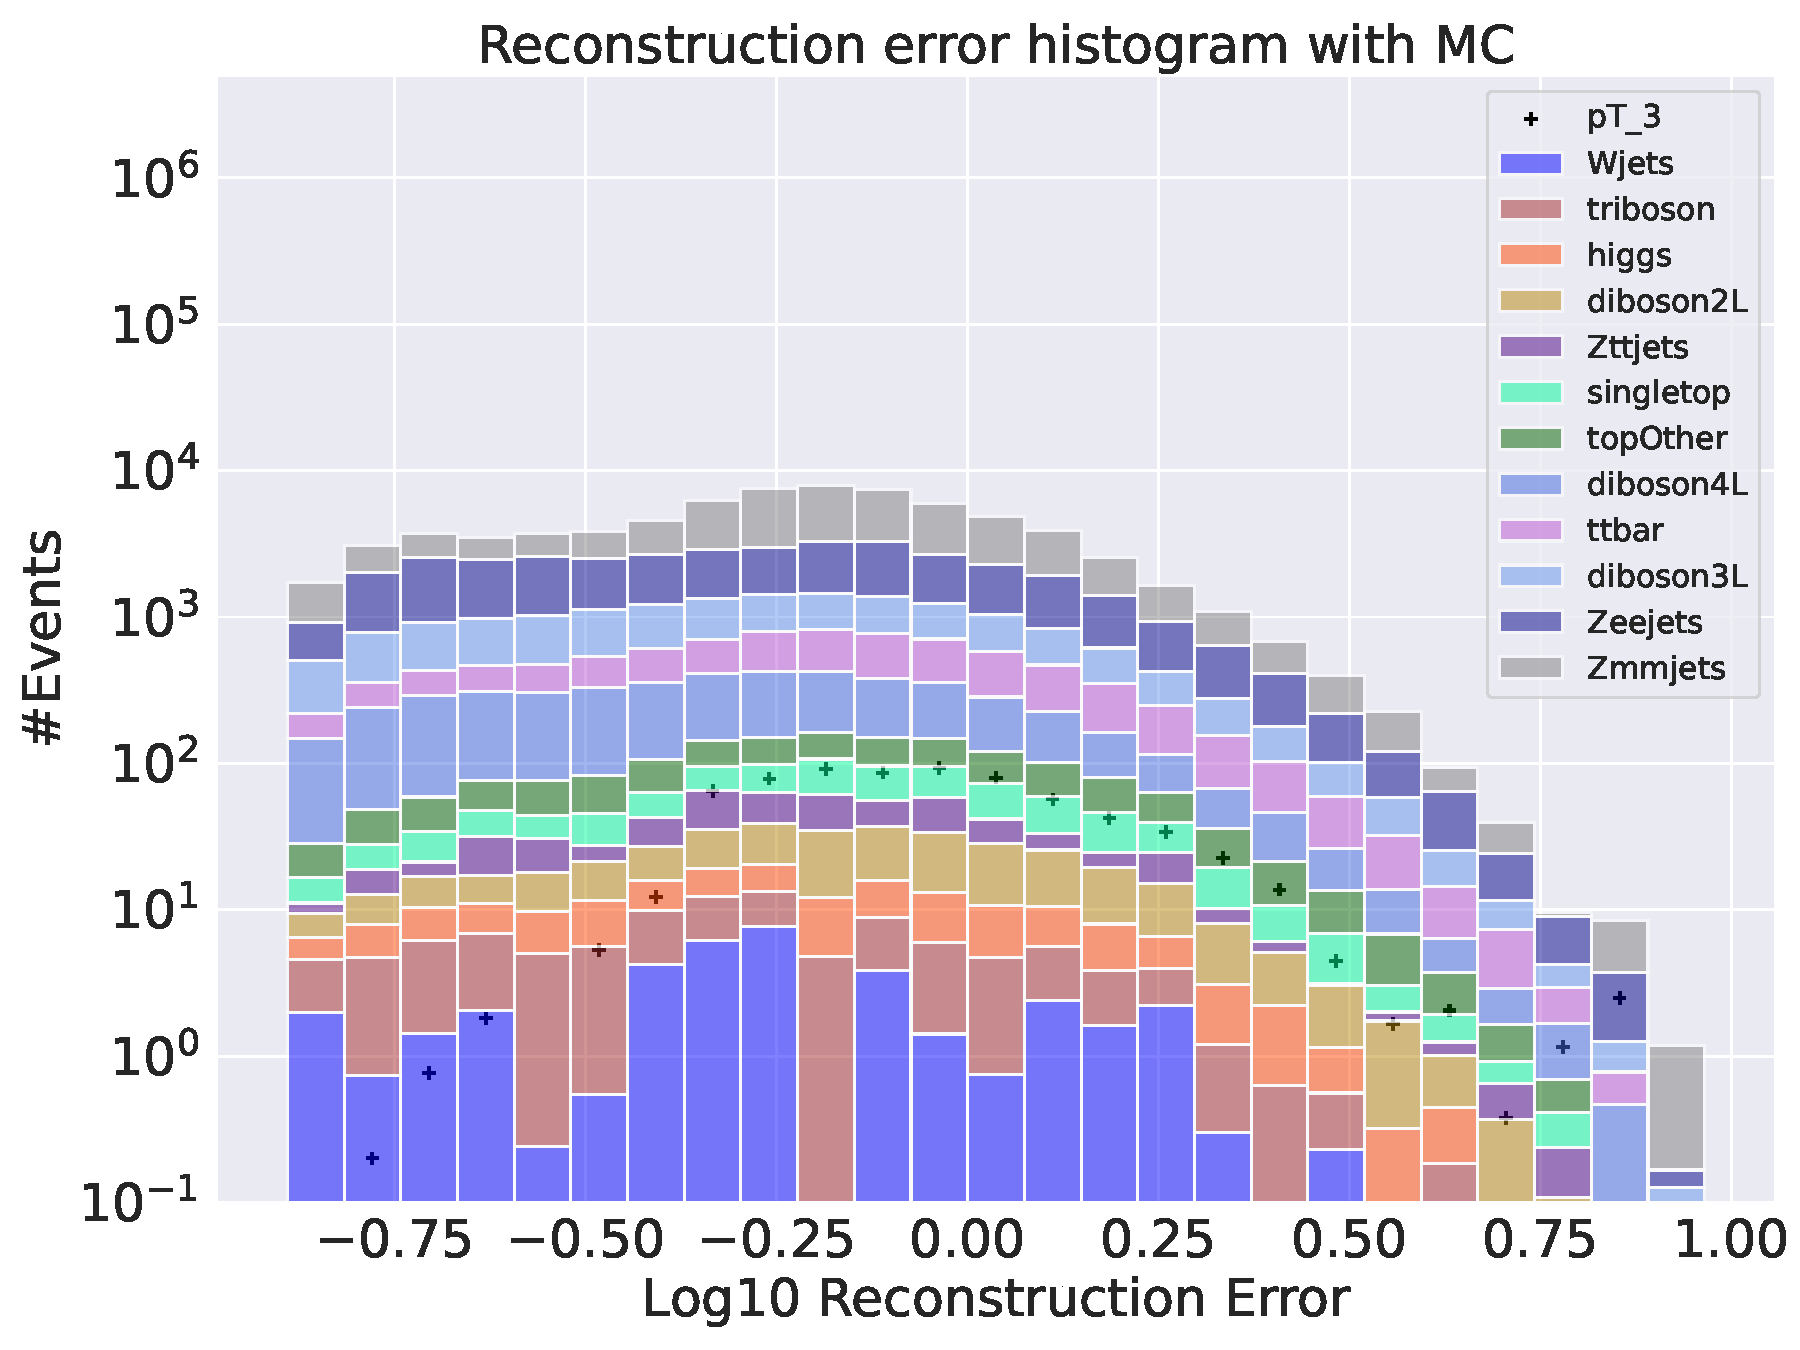
\includegraphics[width=\textwidth]{Figures/VAE_testing/small/b_data_recon_big_rm3_feats_sig_pT_3.pdf}
        \caption{Reconstruction error on validation SM MC from the small variational Autoencoder. Here the signal is a subsample of the validation 
        set where the transverse momentum of the first electron and the first muon has been increased with a scale of $3$. The change of transverse 
        energy has thusly also been changed according to the scaling of transverse momentum. No significant difference in distributions are found. }
        \label{fig:VAE_small_pt_3}
    \end{subfigure}
    \hfill 
    \begin{subfigure}{.45\textwidth}
        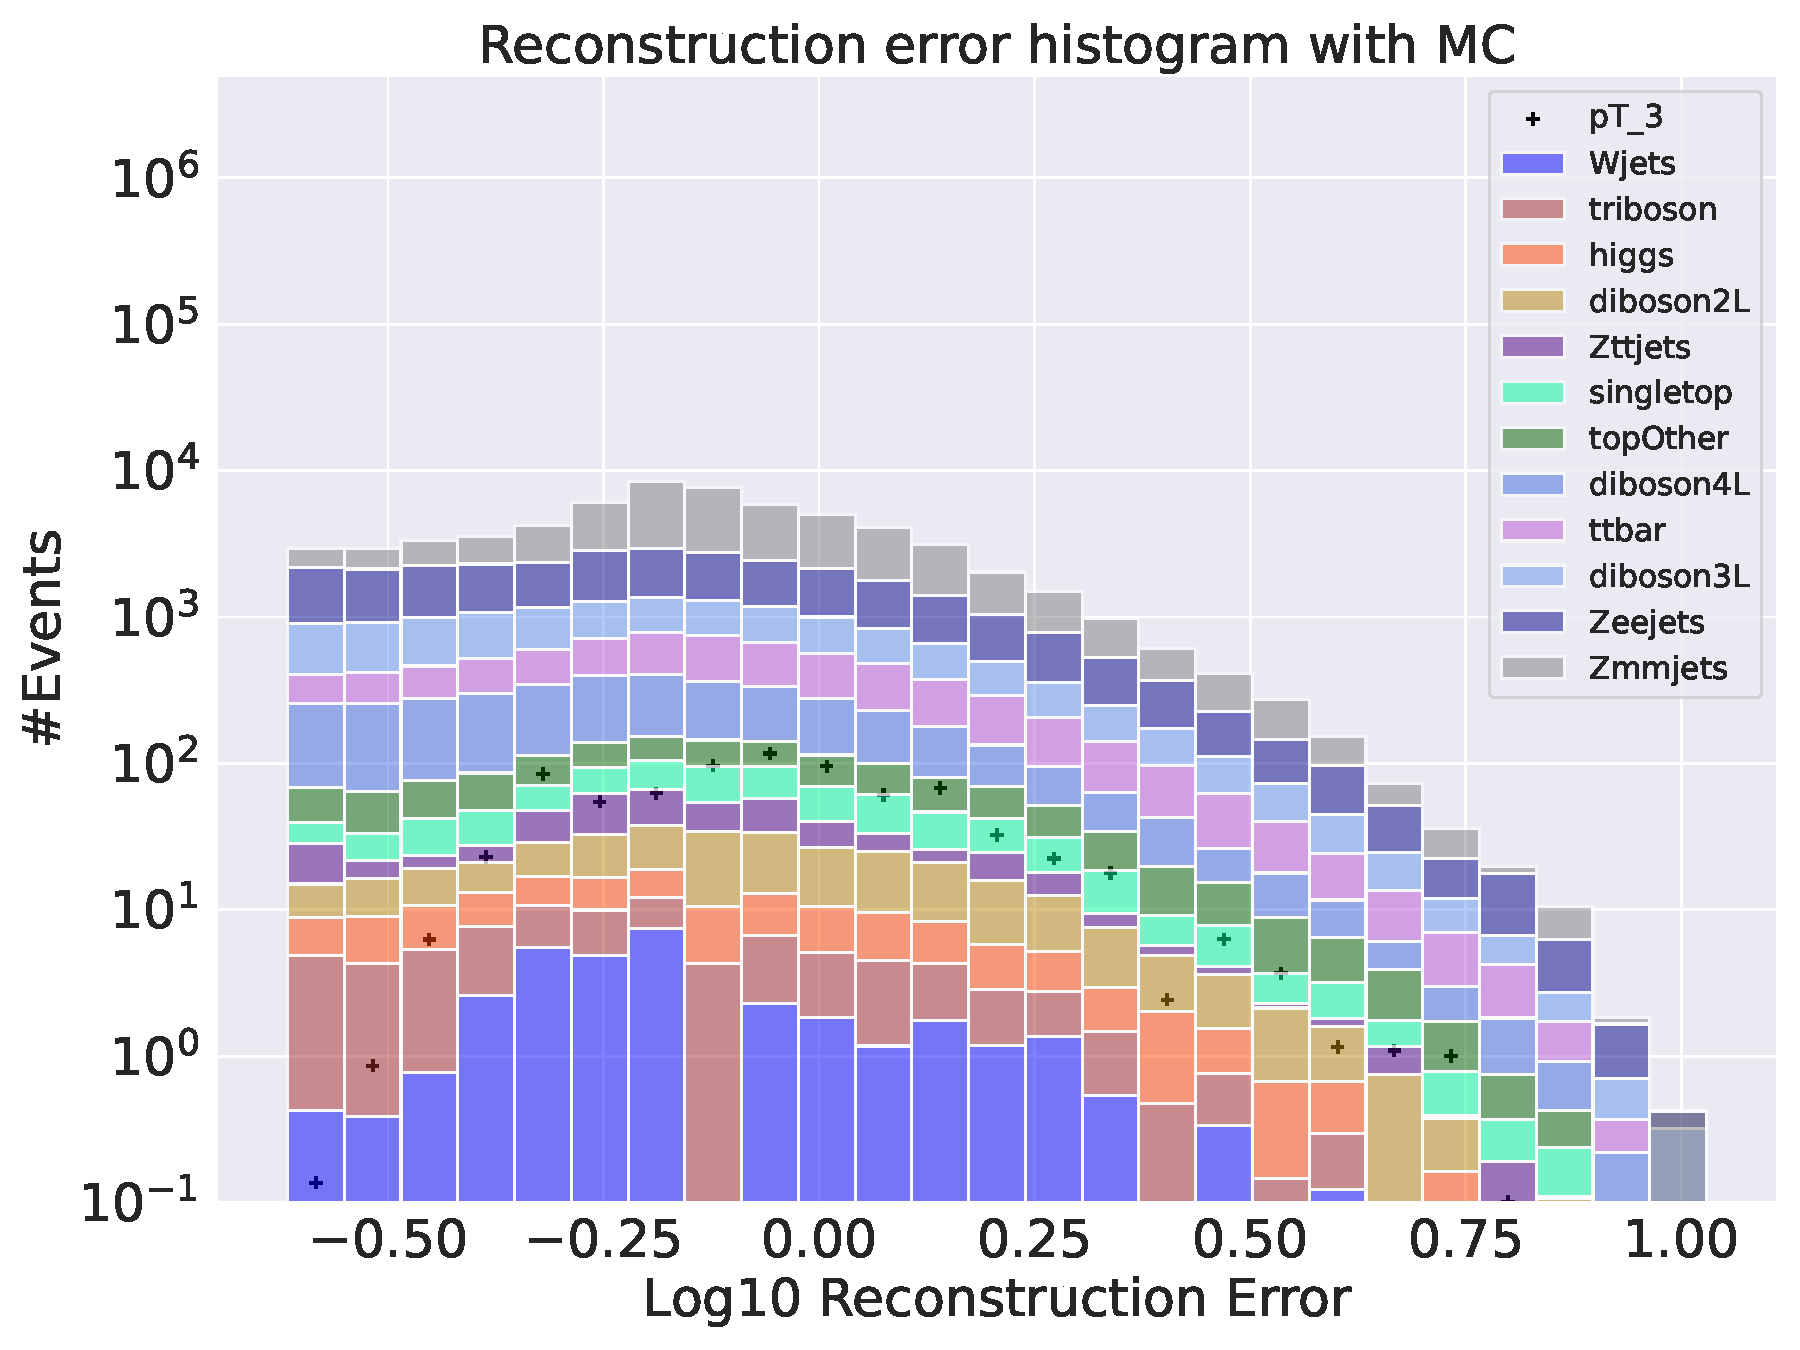
\includegraphics[width=\textwidth]{Figures/VAE_testing/big/b_data_recon_big_rm3_feats_sig_pT_3.pdf}
        \caption{Reconstruction error on validation SM MC from the big variational Autoencoder. Here the signal is a subsample of the validation 
        set where the transverse momentum of the first electron and the first muon has been increased with a scale of $3$. The change of transverse 
        energy has thusly also been changed according to the scaling of transverse momentum. No significant difference in distributions are found. }
        \label{fig:VAE_big_pt_3}
    \end{subfigure}
    \hfill 
    \label{fig:VAE_big_small_pt_3}
\end{figure}

\begin{figure}[h!]
    \centering
    \begin{subfigure}{.45\textwidth}
        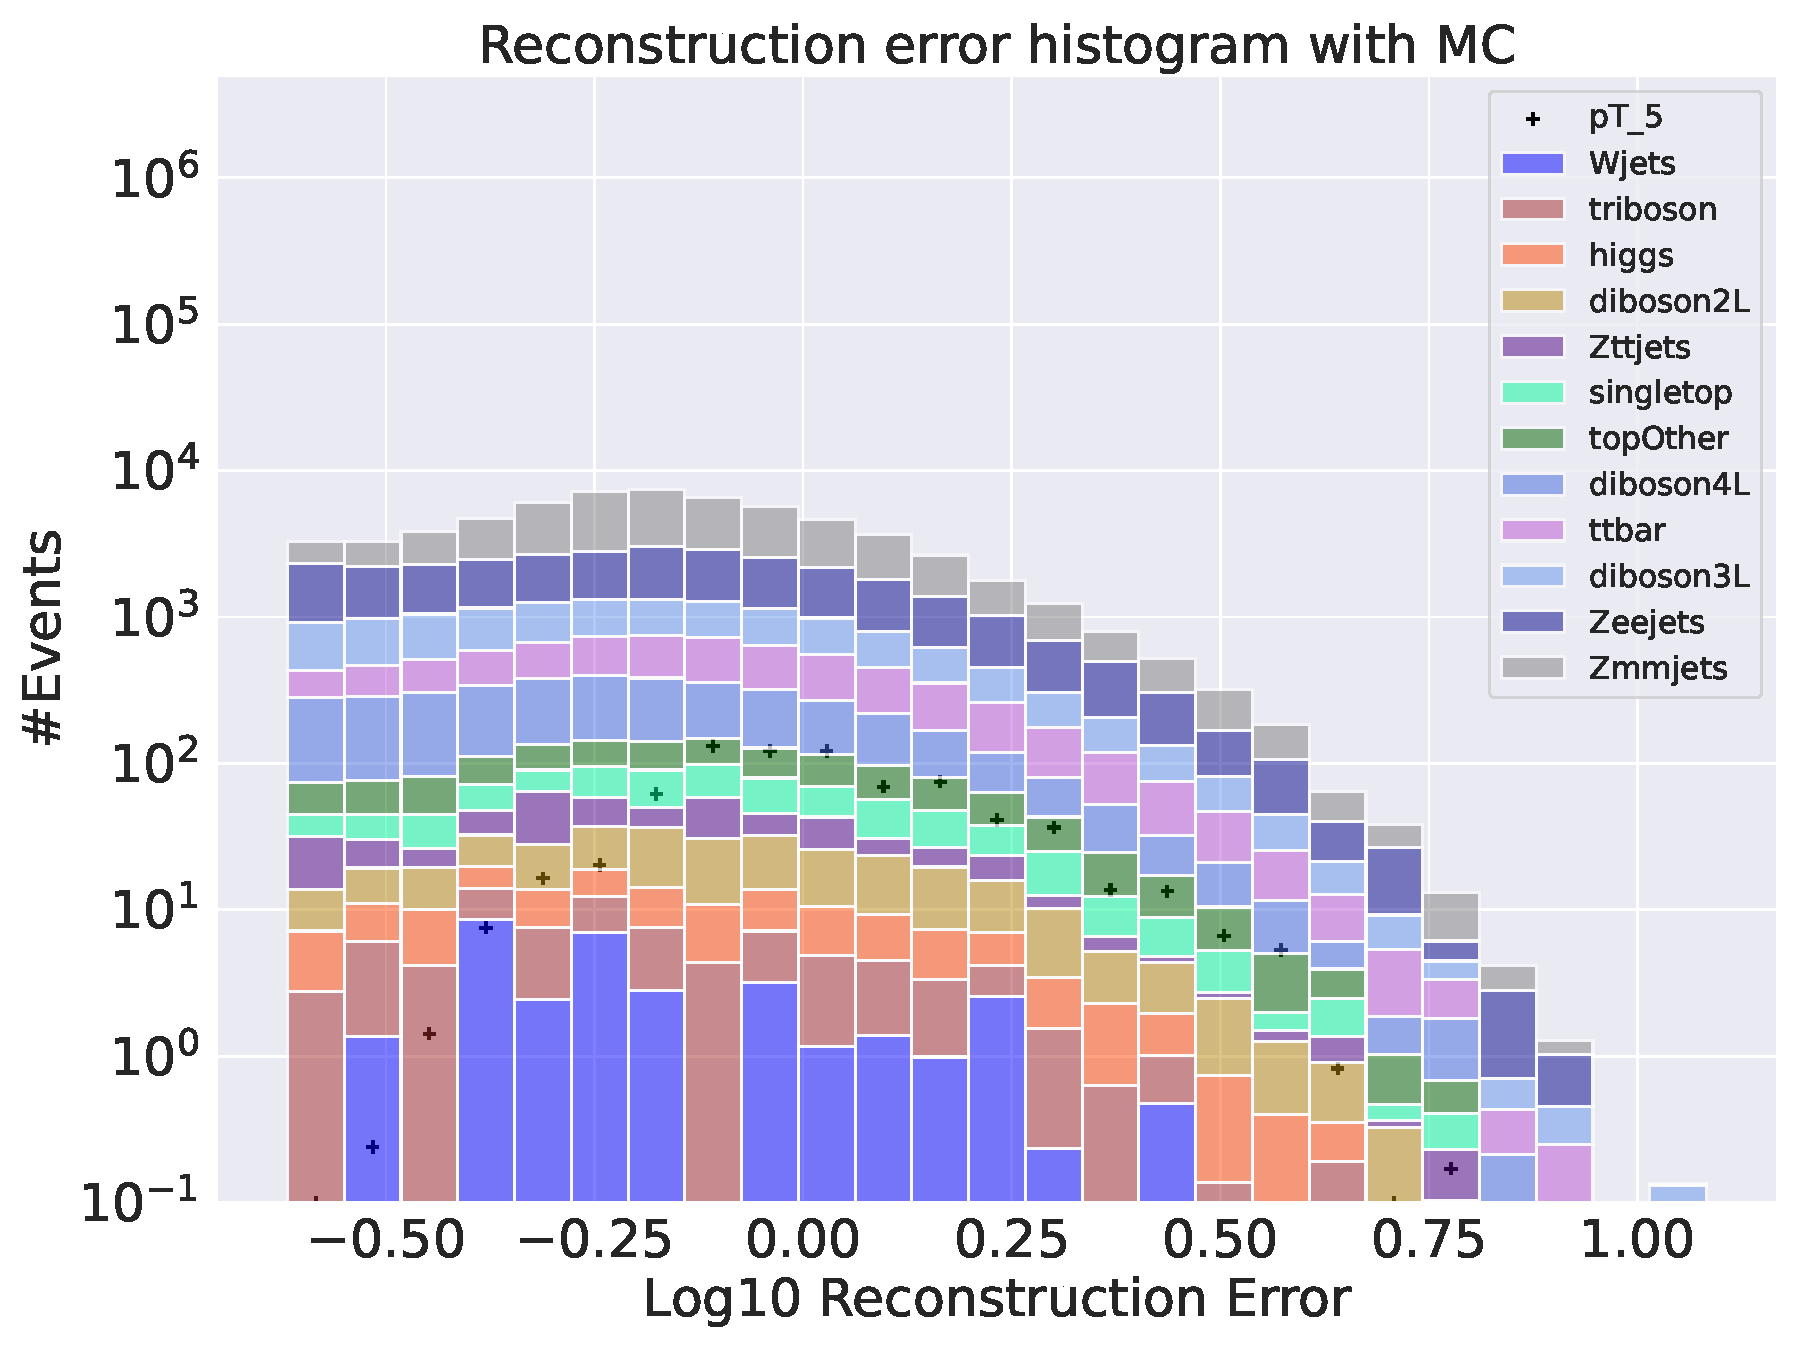
\includegraphics[width=\textwidth]{Figures/VAE_testing/small/b_data_recon_big_rm3_feats_sig_pT_5.pdf}
        \caption{Reconstruction error on validation SM MC from the small variational Autoencoder.Here the signal is a subsample of the validation 
        set where the transverse momentum of the first electron and the first muon has been increased with a scale of $5$. The change of transverse 
        energy has thusly also been changed according to the scaling of transverse momentum.  No significant difference in distributions are found. }
        \label{fig:VAE_small_pt_5}
    \end{subfigure}
    \hfill 
    \begin{subfigure}{.45\textwidth}
        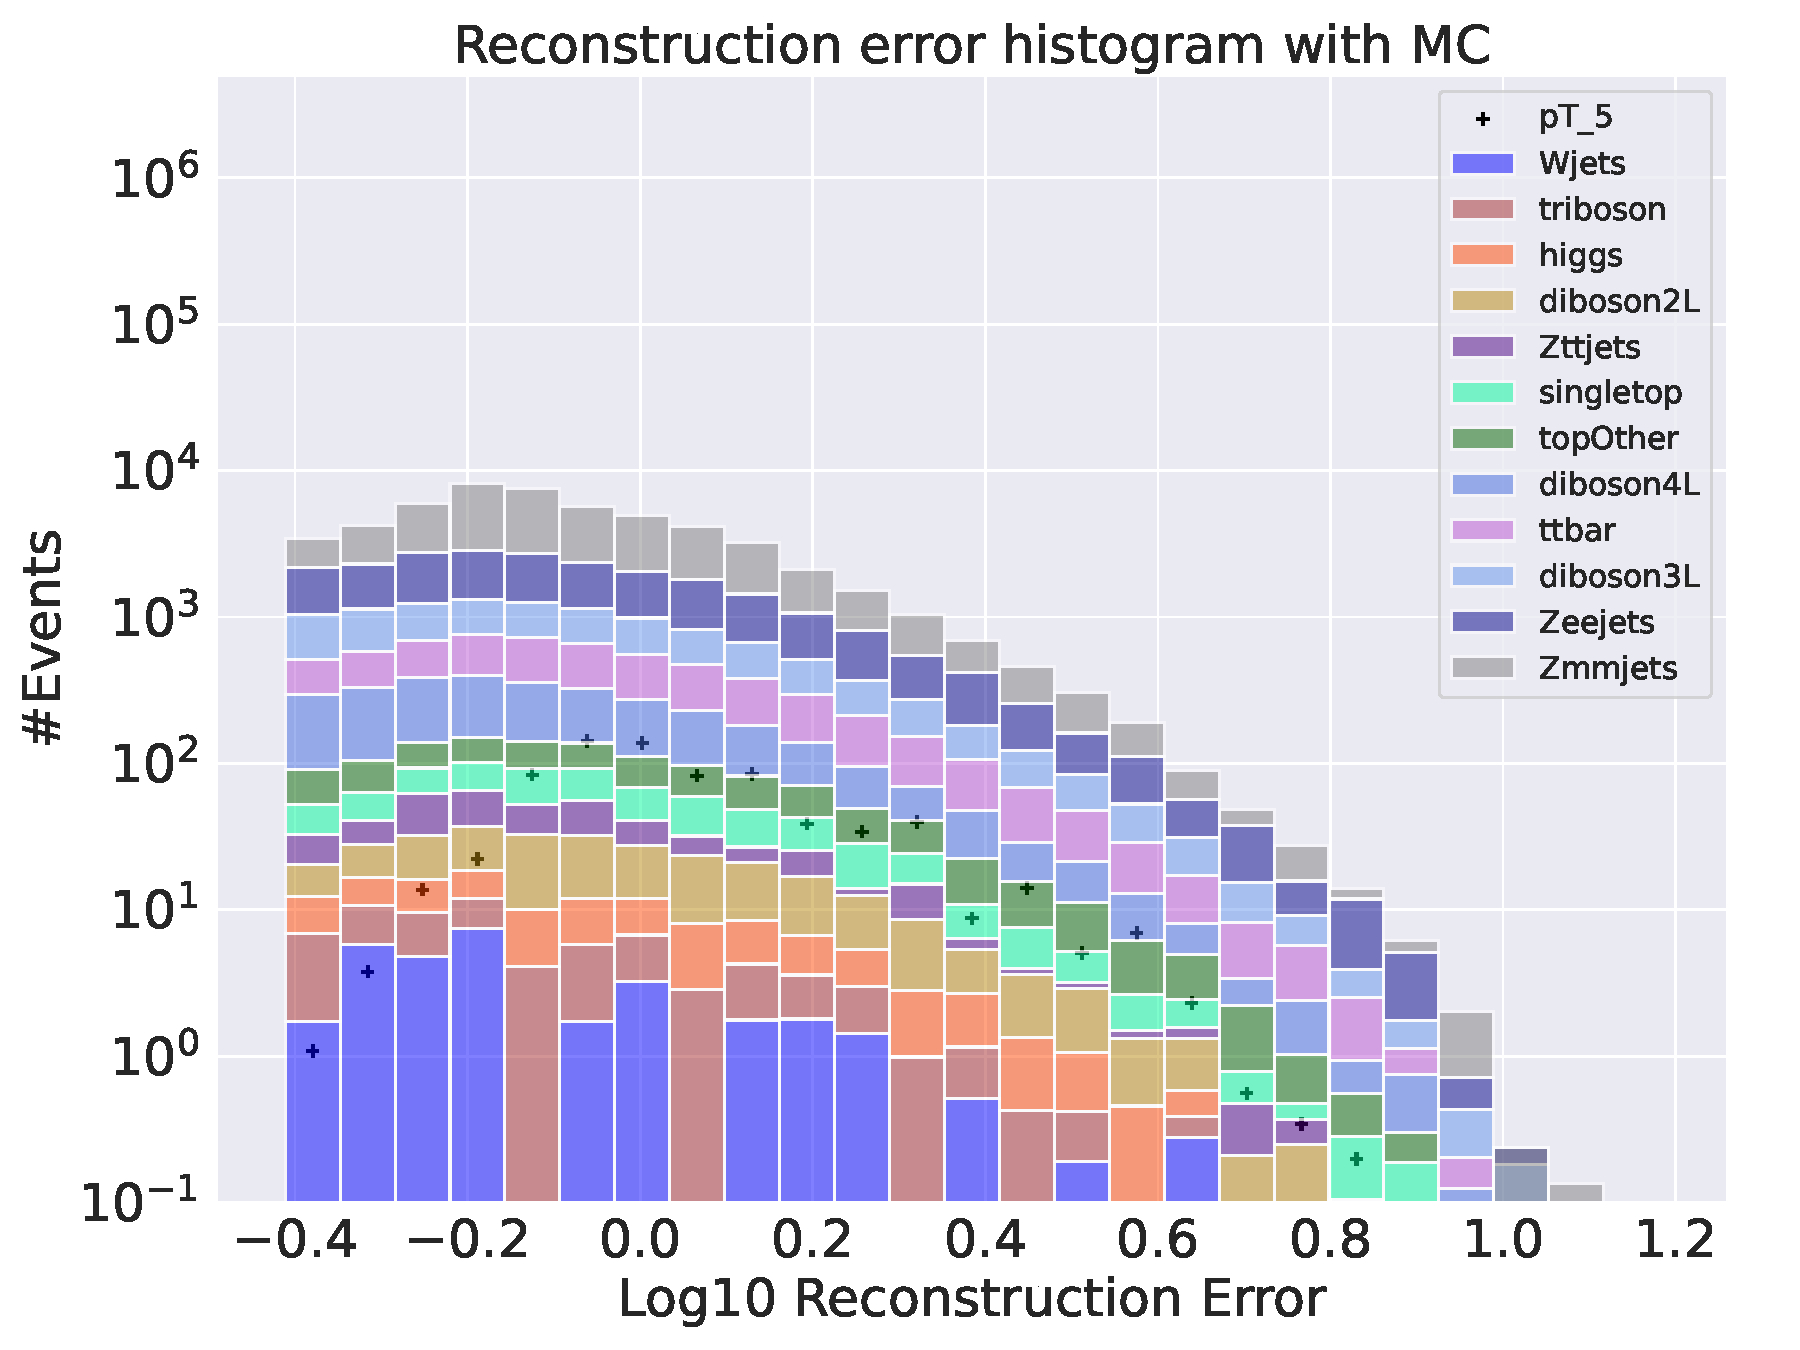
\includegraphics[width=\textwidth]{Figures/VAE_testing/big/b_data_recon_big_rm3_feats_sig_pT_5.pdf}
        \caption{Reconstruction error on validation SM MC from the big variational Autoencoder. Here the signal is a subsample of the validation 
        set where the transverse momentum of the first electron and the first muon has been increased with a scale of $5$. The change of transverse 
        energy has thusly also been changed according to the scaling of transverse momentum. No significant difference in distributions are found. }
        \label{fig:VAE_big_pt_5}
    \end{subfigure}
    \hfill 
    \label{fig:VAE_big_small_pt_5}
\end{figure}


\begin{figure}[h!]
    \centering
    \begin{subfigure}{.45\textwidth}
        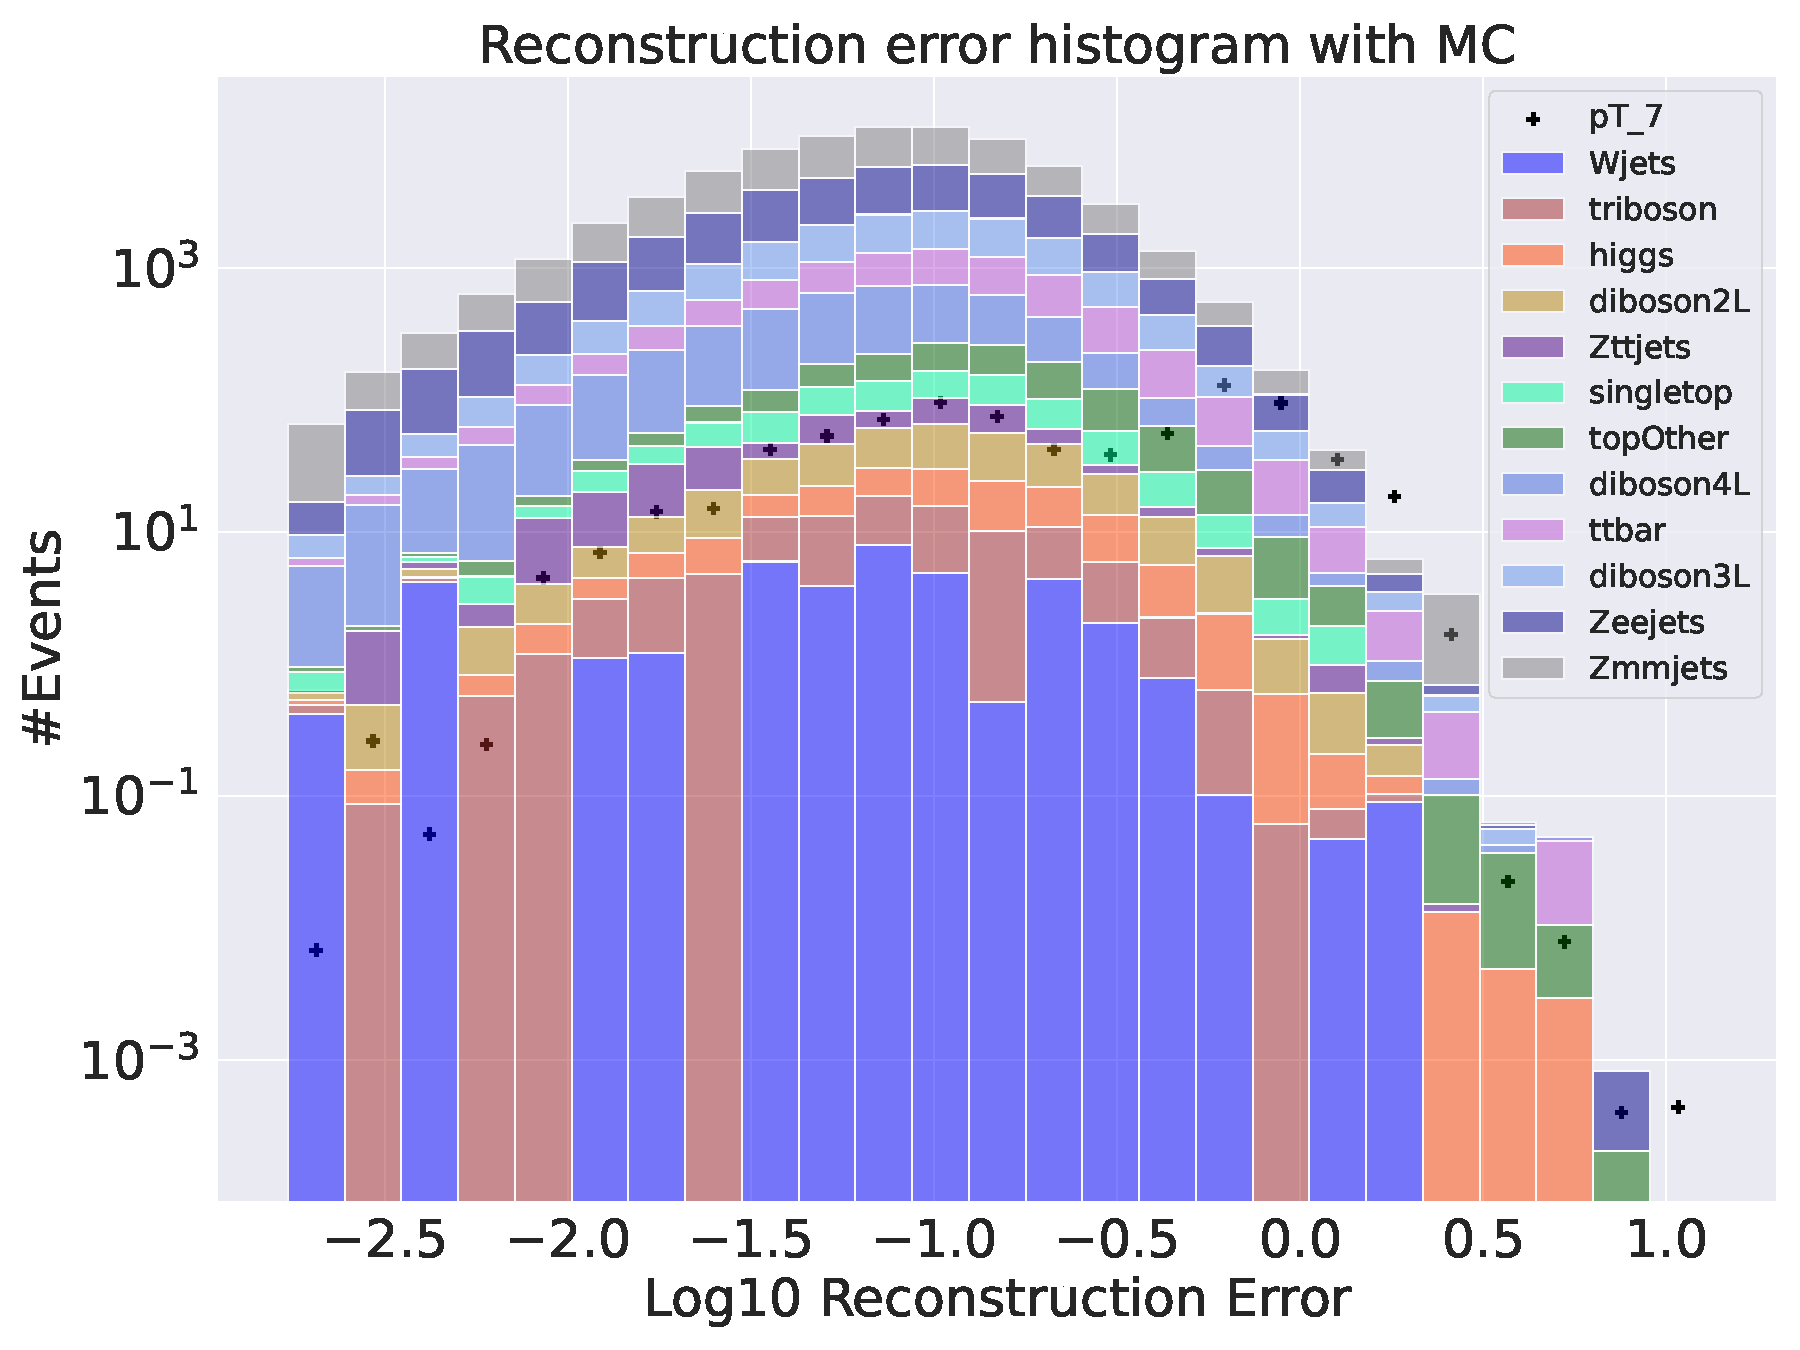
\includegraphics[width=\textwidth]{Figures/VAE_testing/small/b_data_recon_big_rm3_feats_sig_pT_7.pdf}
        \caption{Reconstruction error on validation SM MC from the small variational Autoencoder. Here the signal is a subsample of the validation 
        set where the transverse momentum of the first electron and the first muon has been increased with a scale of $7$. The change of transverse 
        energy has thusly also been changed according to the scaling of transverse momentum. No significant difference in distributions are found. }
        \label{fig:VAE_small_pt_7}
    \end{subfigure}
    \hfill 
    \begin{subfigure}{.45\textwidth}
        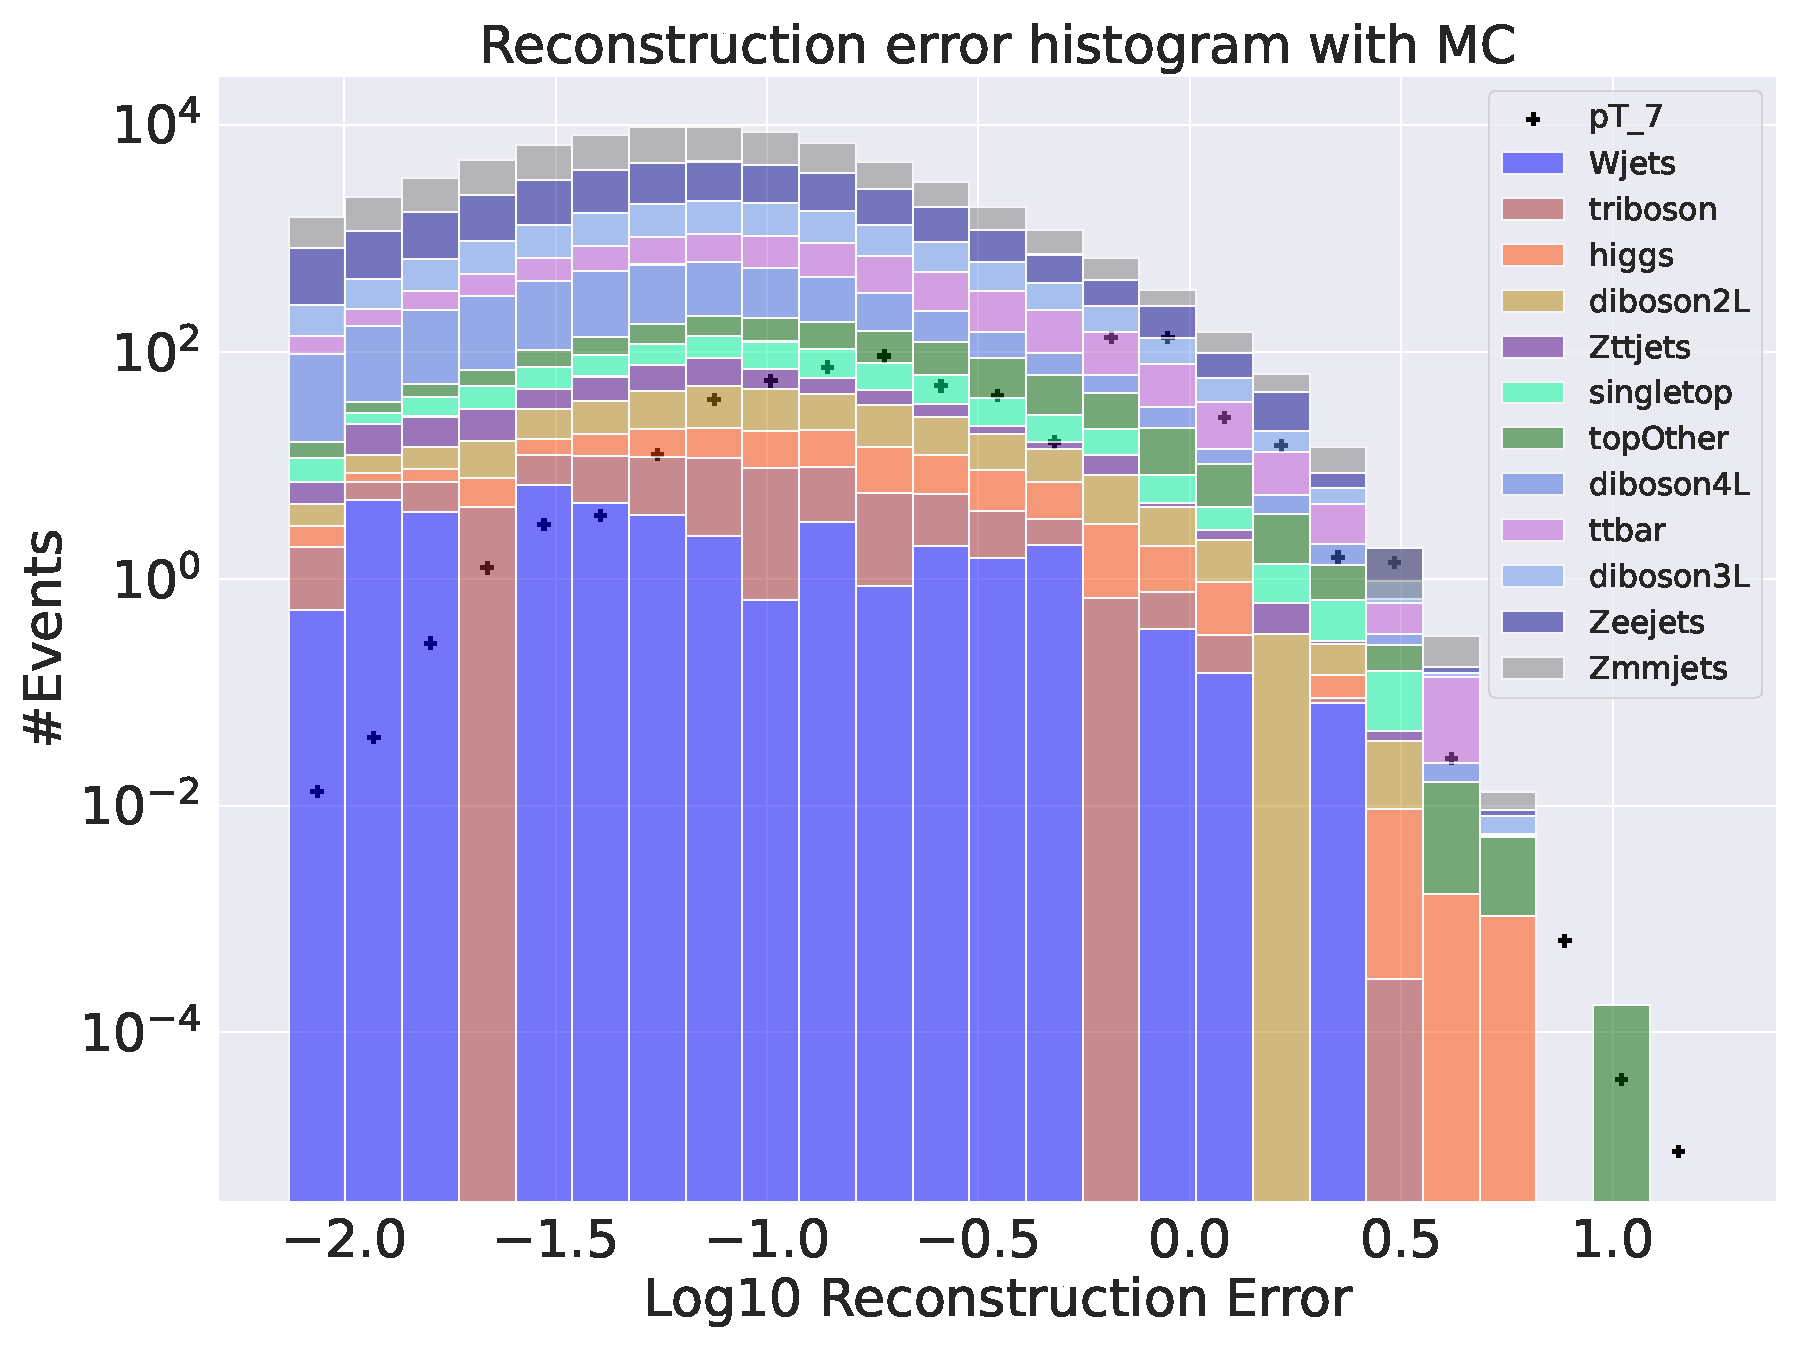
\includegraphics[width=\textwidth]{Figures/VAE_testing/big/b_data_recon_big_rm3_feats_sig_pT_7.pdf}
        \caption{Reconstruction error on validation SM MC from the big variational Autoencoder. Here the signal is a subsample of the validation 
        set where the transverse momentum of the first electron and the first muon has been increased with a scale of $7$. The change of transverse 
        energy has thusly also been changed according to the scaling of transverse momentum. No significant difference in distributions are found. }
        \label{fig:VAE_big_pt_7}
    \end{subfigure}
    \hfill 
    \label{fig:VAE_big_small_pt_7}
\end{figure}

\begin{figure}[h!]
    \centering
    \begin{subfigure}{.45\textwidth}
        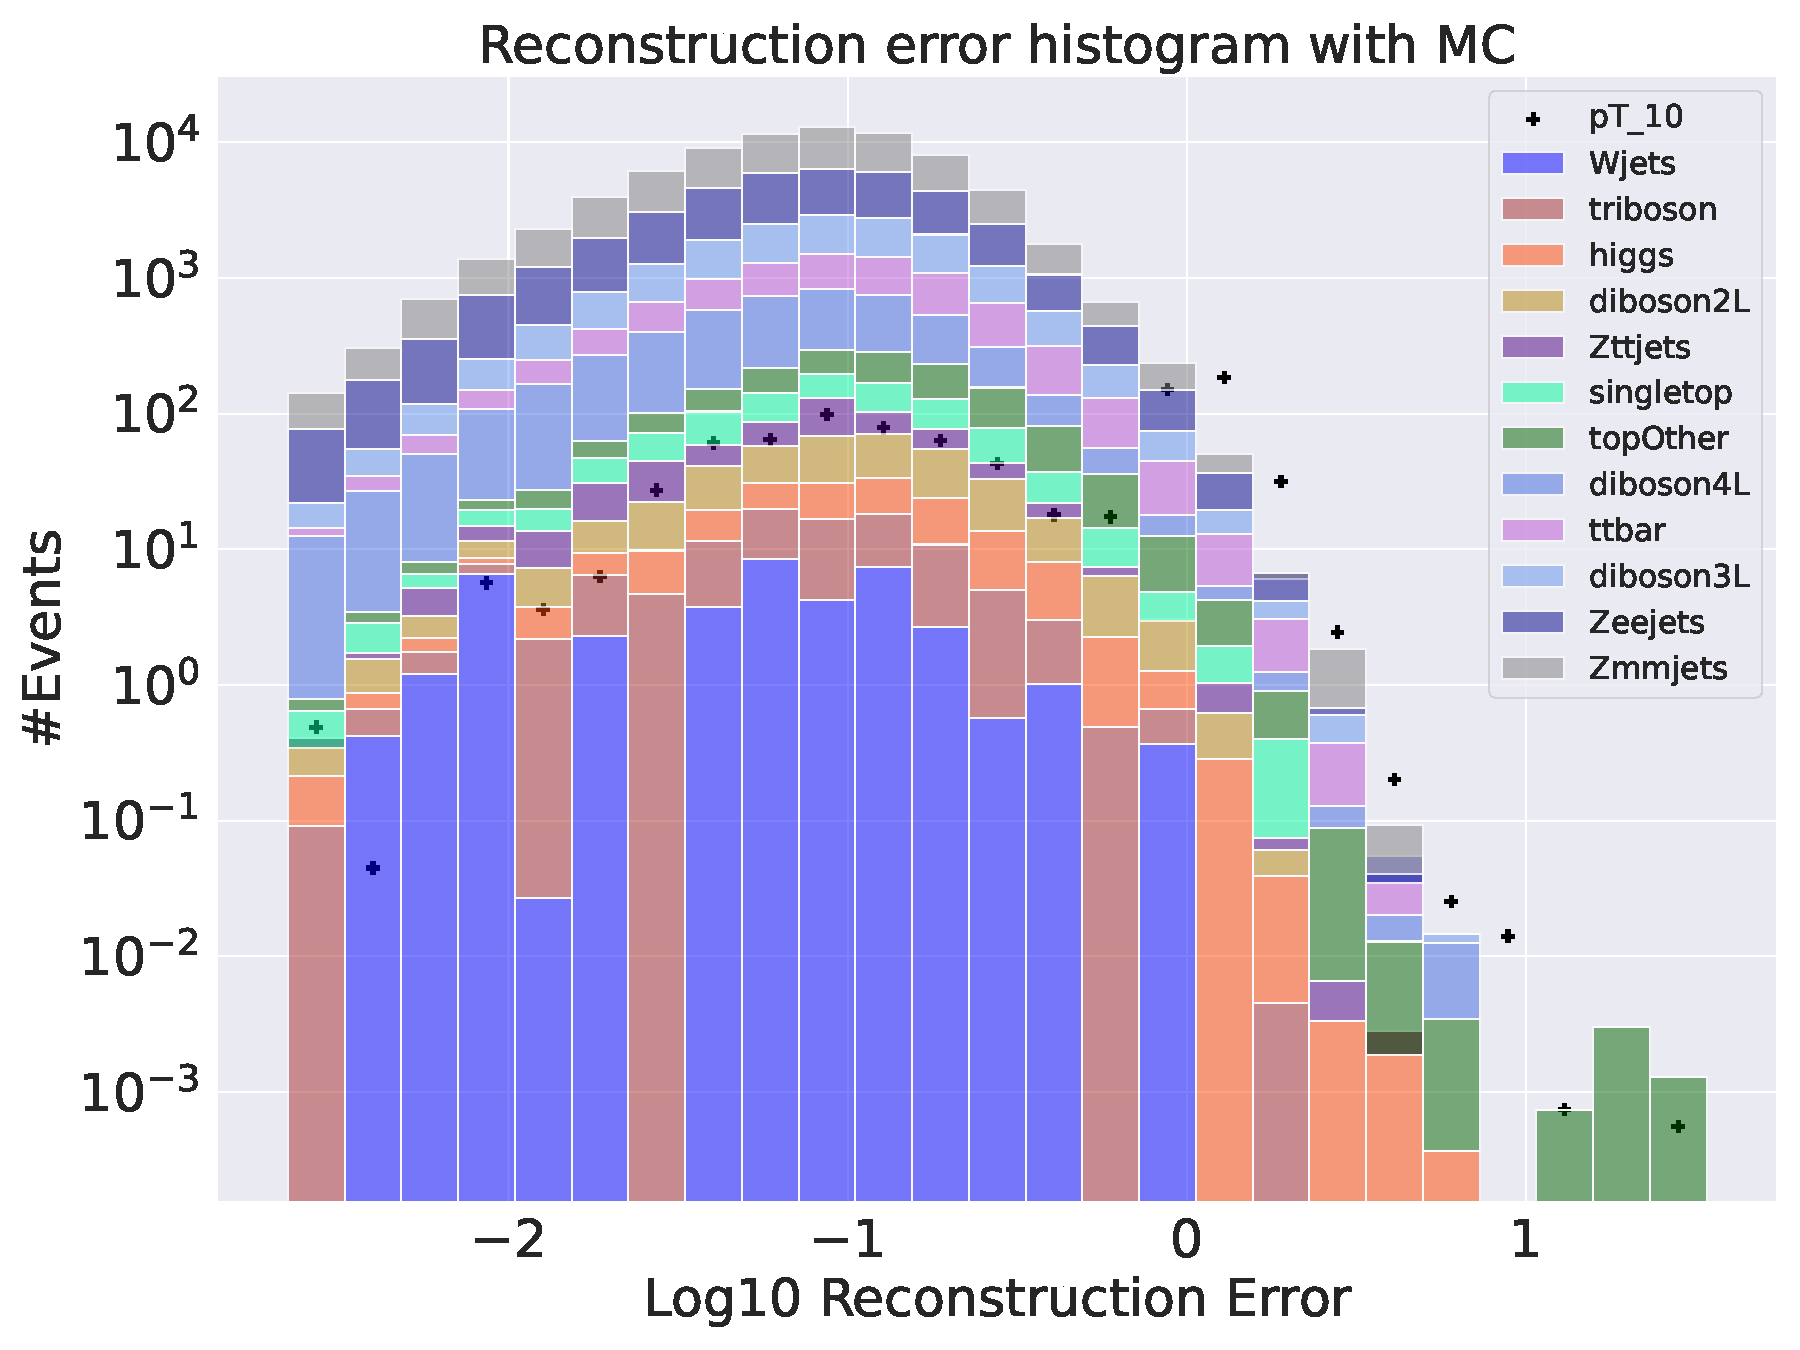
\includegraphics[width=\textwidth]{Figures/VAE_testing/small/b_data_recon_big_rm3_feats_sig_pT_10.pdf}
        \caption{Reconstruction error on validation SM MC from the small variational Autoencoder. Here the signal is a subsample of the validation 
        set where the transverse momentum of the first electron and the first muon has been increased with a scale of $10$. The change of transverse 
        energy has thusly also been changed according to the scaling of transverse momentum. No significant difference in distributions are found. }
        \label{fig:VAE_small_pt_10}
    \end{subfigure}
    \hfill 
    \begin{subfigure}{.45\textwidth}
        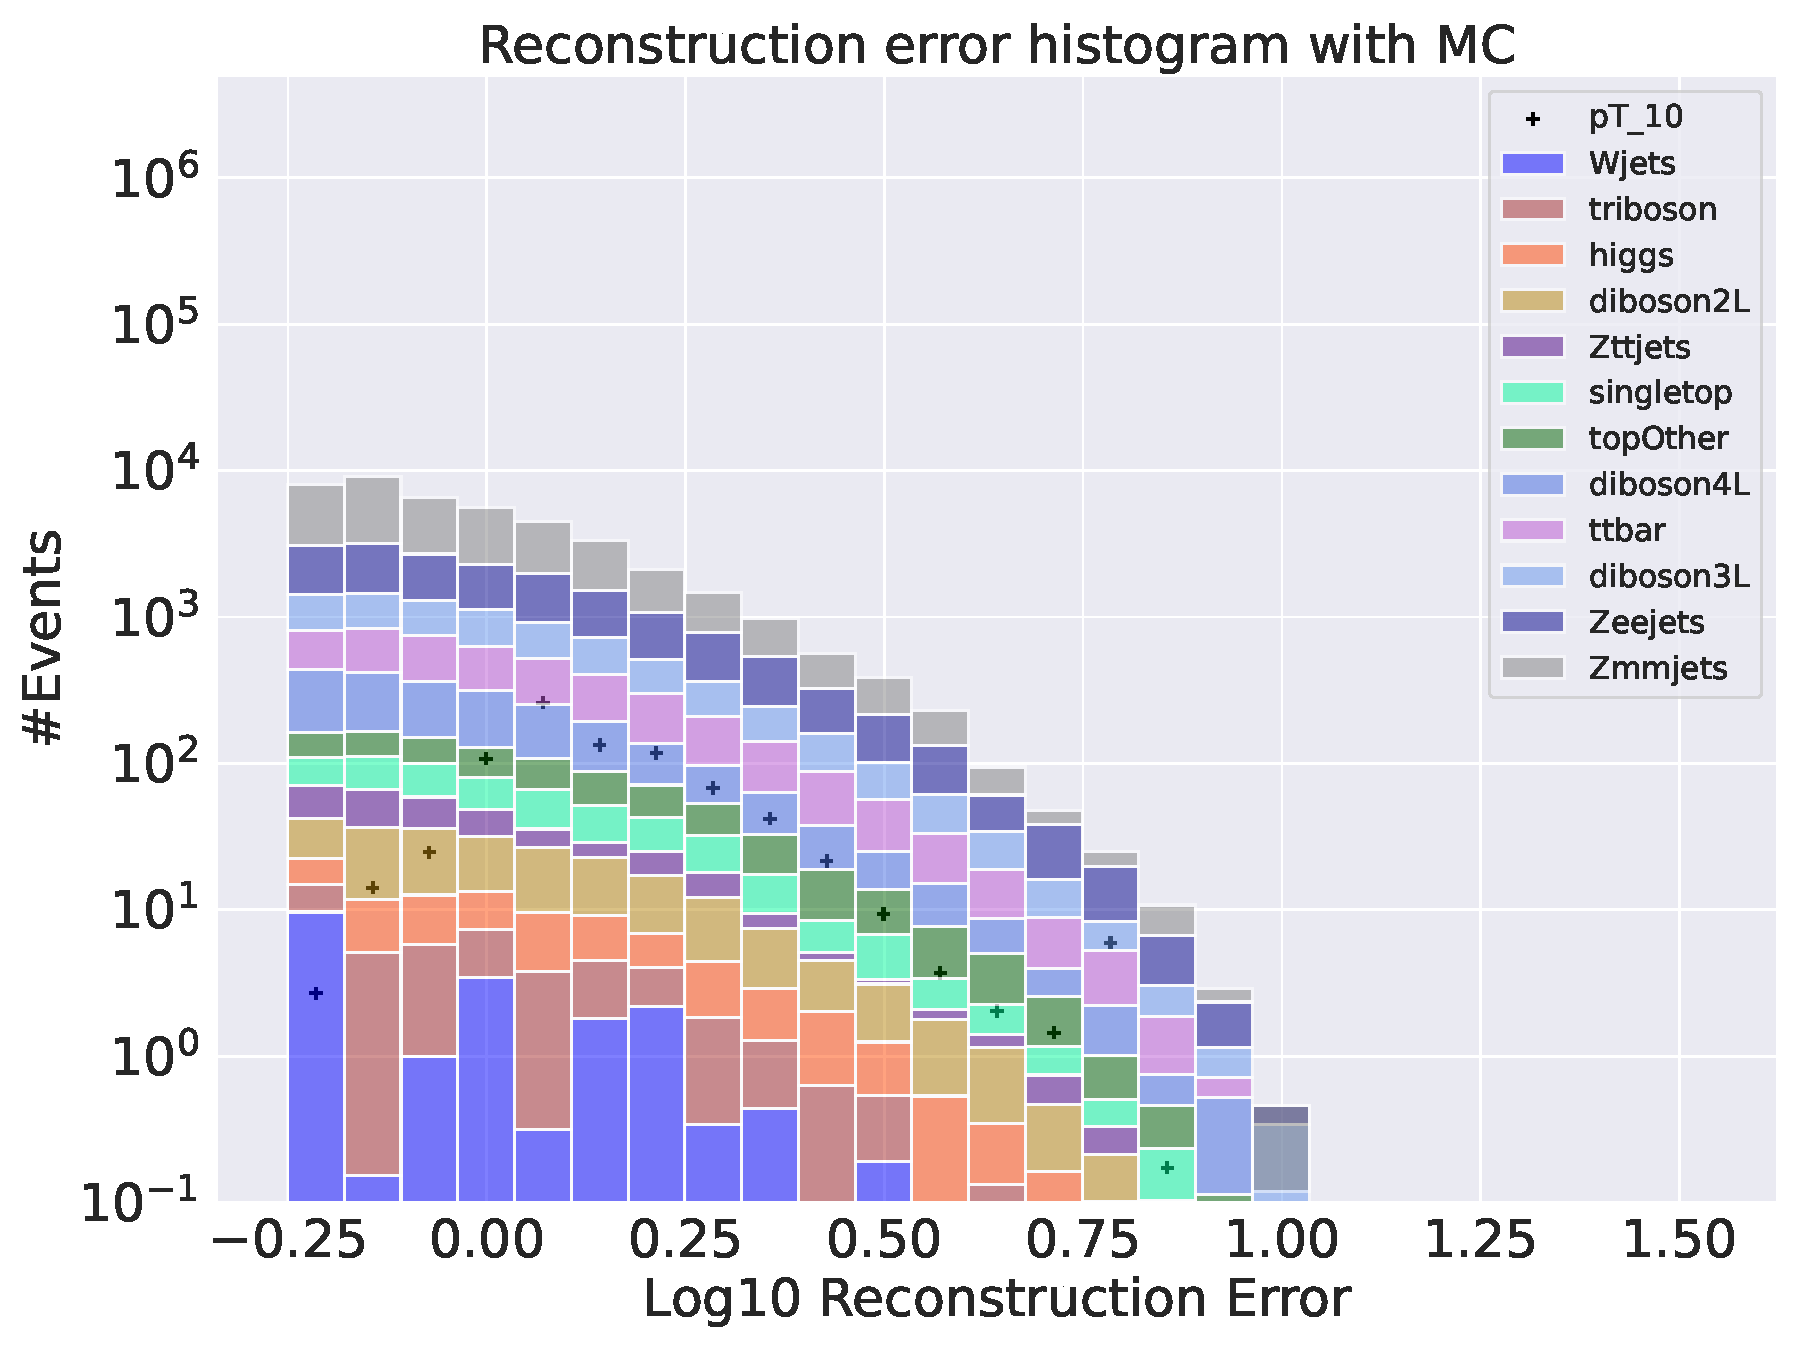
\includegraphics[width=\textwidth]{Figures/VAE_testing/big/b_data_recon_big_rm3_feats_sig_pT_10.pdf}
        \caption{Reconstruction error on validation SM MC from the big variational Autoencoder. Here the signal is a subsample of the validation 
        set where the transverse momentum of the first electron and the first muon has been increased with a scale of $10$. The change of transverse 
        energy has thusly also been changed according to the scaling of transverse momentum. No significant difference in distributions are found. }
        \label{fig:VAE_big_pt_10}
    \end{subfigure}
    \hfill 
    \label{fig:VAE_big_small_pt_10}
\end{figure}

\newpage